\documentclass{article}
\usepackage{graphicx}
\usepackage{listings}
\usepackage{xcolor}
\usepackage{hyperref}
\usepackage{geometry}
\geometry{a4paper, margin=1in}
\title{Grafici dell'utilizzo di memoria heap da parte degli algoritmi di ricerca}
\author{Adriano Oliviero}
\date{	oday}
\begin{document}
\maketitle
\tableofcontents
\newpage
\section{Grafici e Risultati}
Di seguito sono riportati alcuni grafici che visualizzano i risultati sperimentali degli algoritmi di ricerca applicati ai dataset:
\subsection{Dataset: soc-sign-bitcoinalpha.csv.gz}
\subsection{Dataset: email-Enron.txt.gz}
\subsection{Dataset: com-youtube.ungraph.txt.gz}
\subsection{Dataset: roadNet-CA.txt.gz}
\subsection{Dataset: as-skitter.txt.gz}
\subsection{Dataset: cit-Patents.txt.gz}
\subsection{Dataset: com-lj.ungraph.txt.gz}
\subsubsection{Algoritmo di ricerca: breadth-first}
\begin{figure}[h]\centering
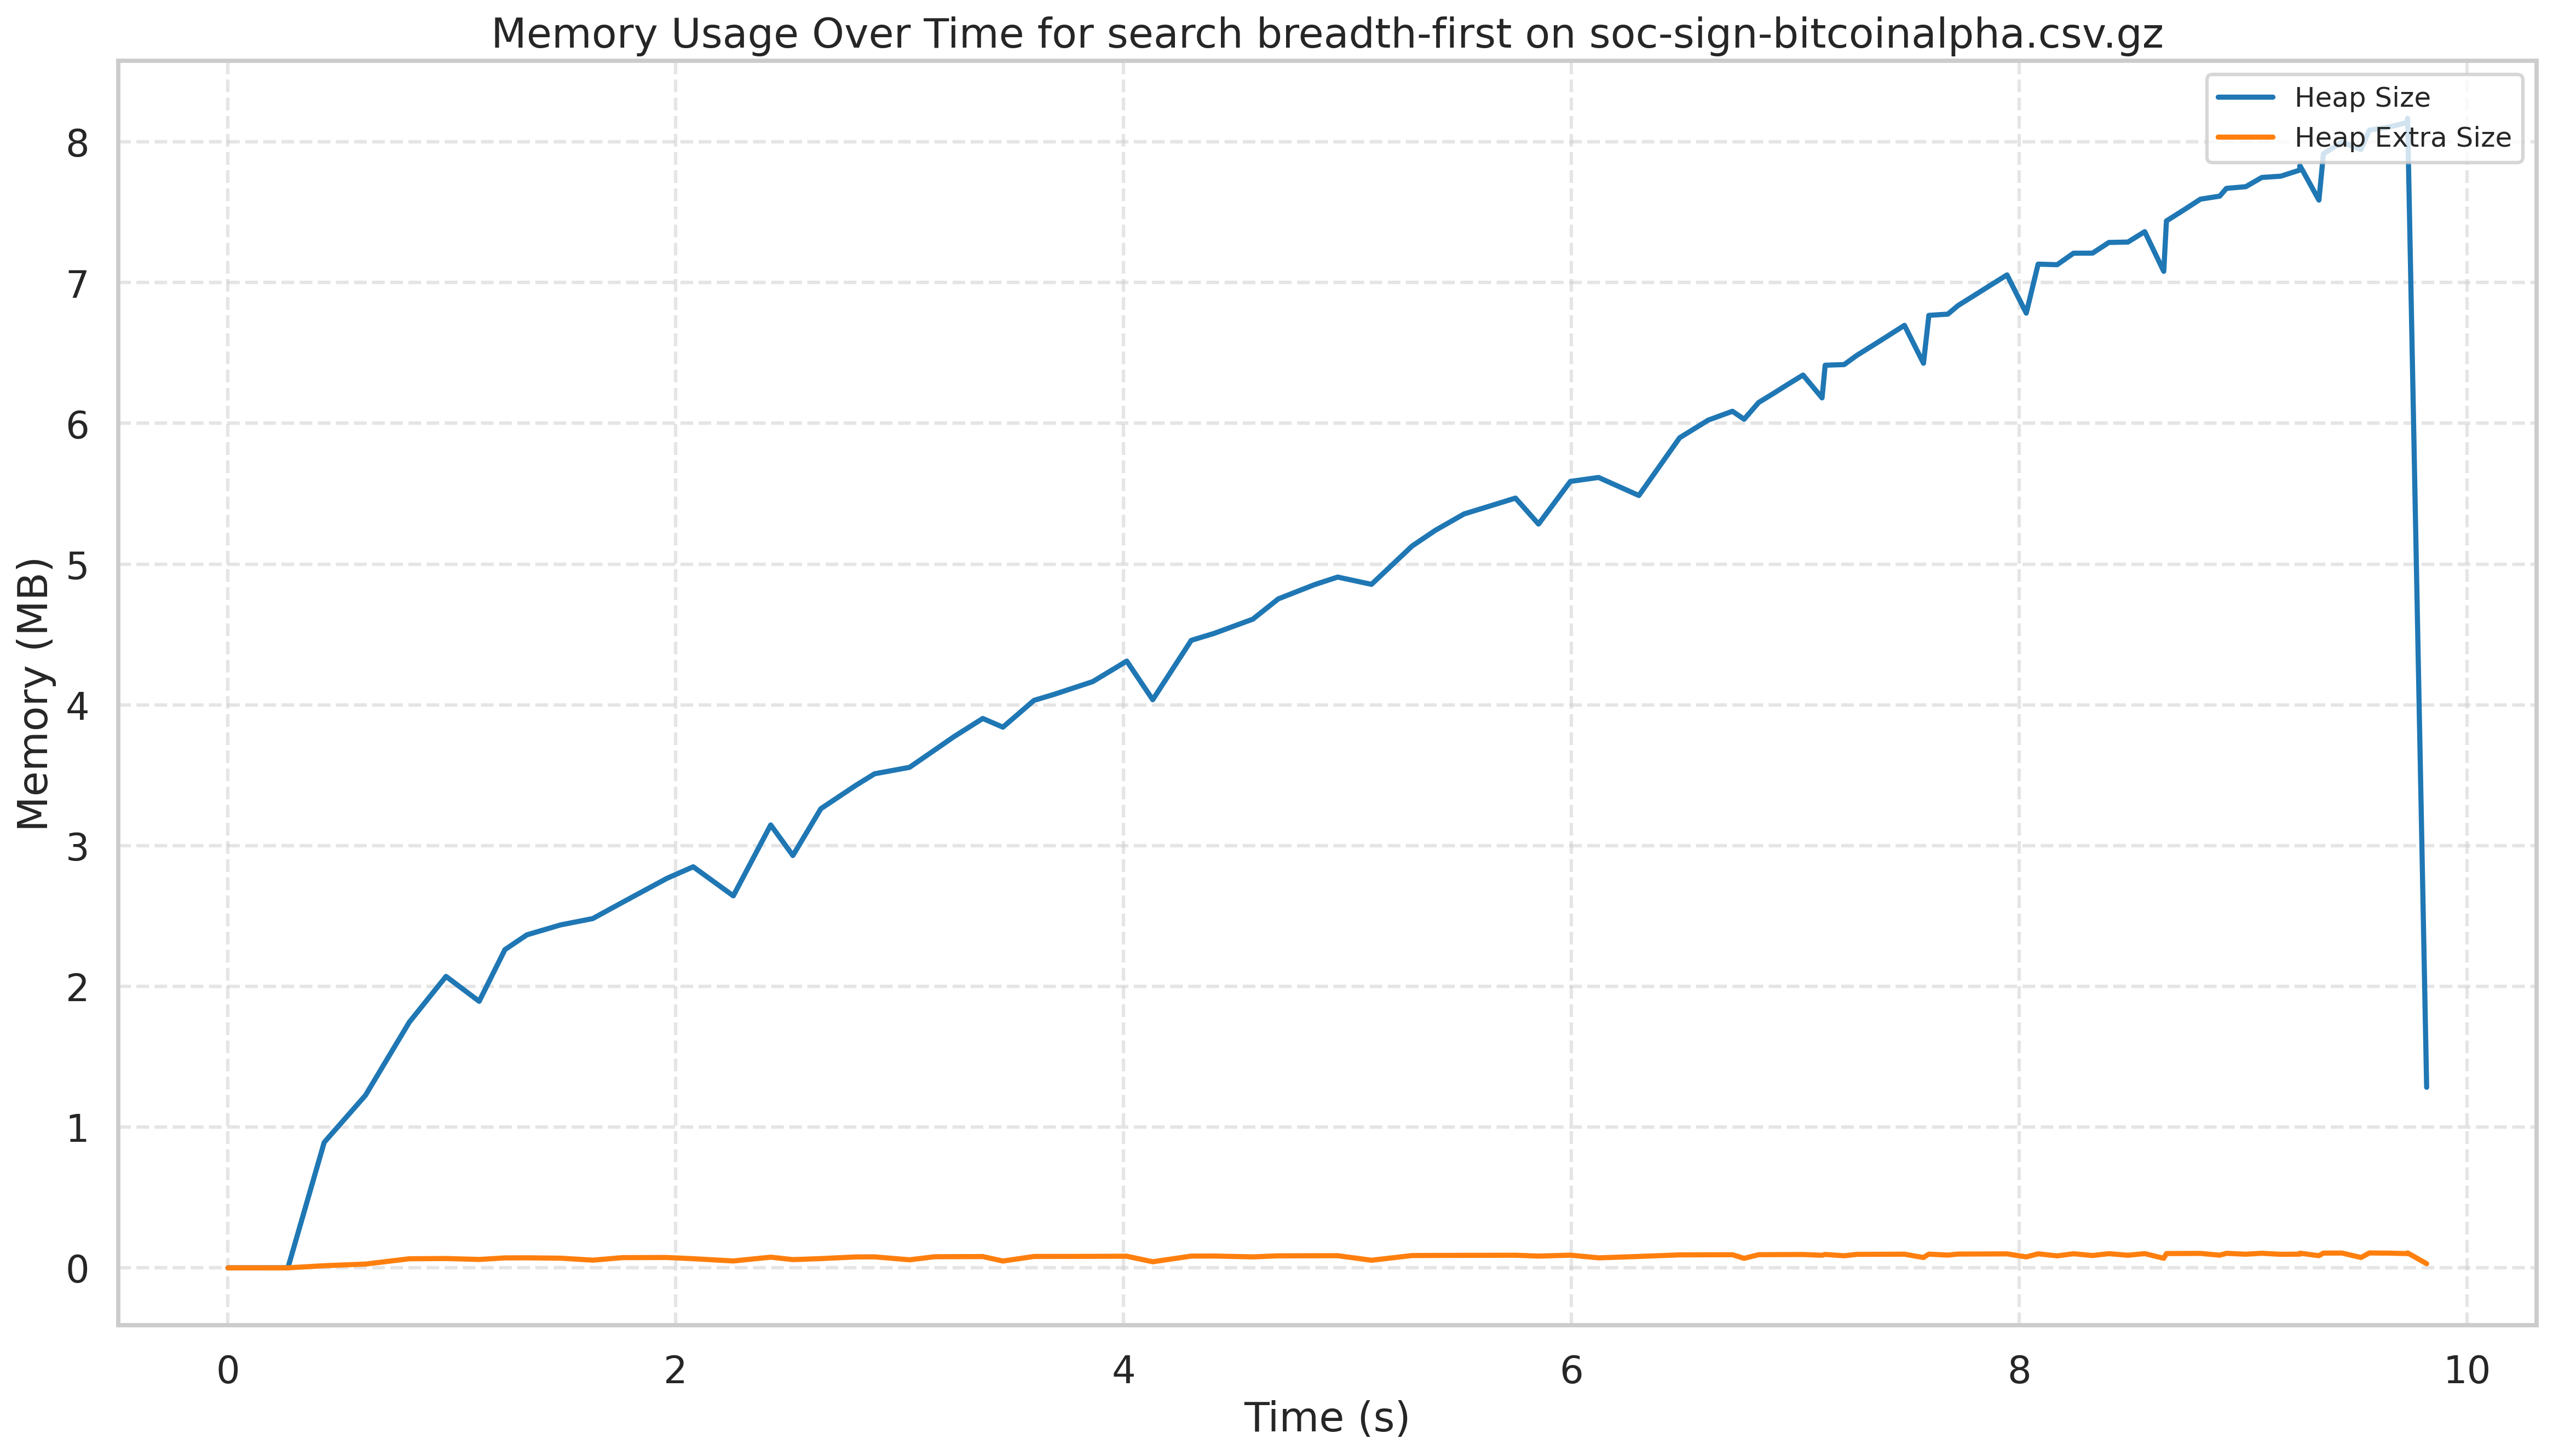
\includegraphics[width=\textwidth]{../plots/soc-sign-bitcoinalpha.csv_breadth-first.png}
\caption{Grafico: breadth-first su com-lj.ungraph}
\end{figure}
\subsubsection{Algoritmo di ricerca: uniform-cost}
\begin{figure}[h]\centering
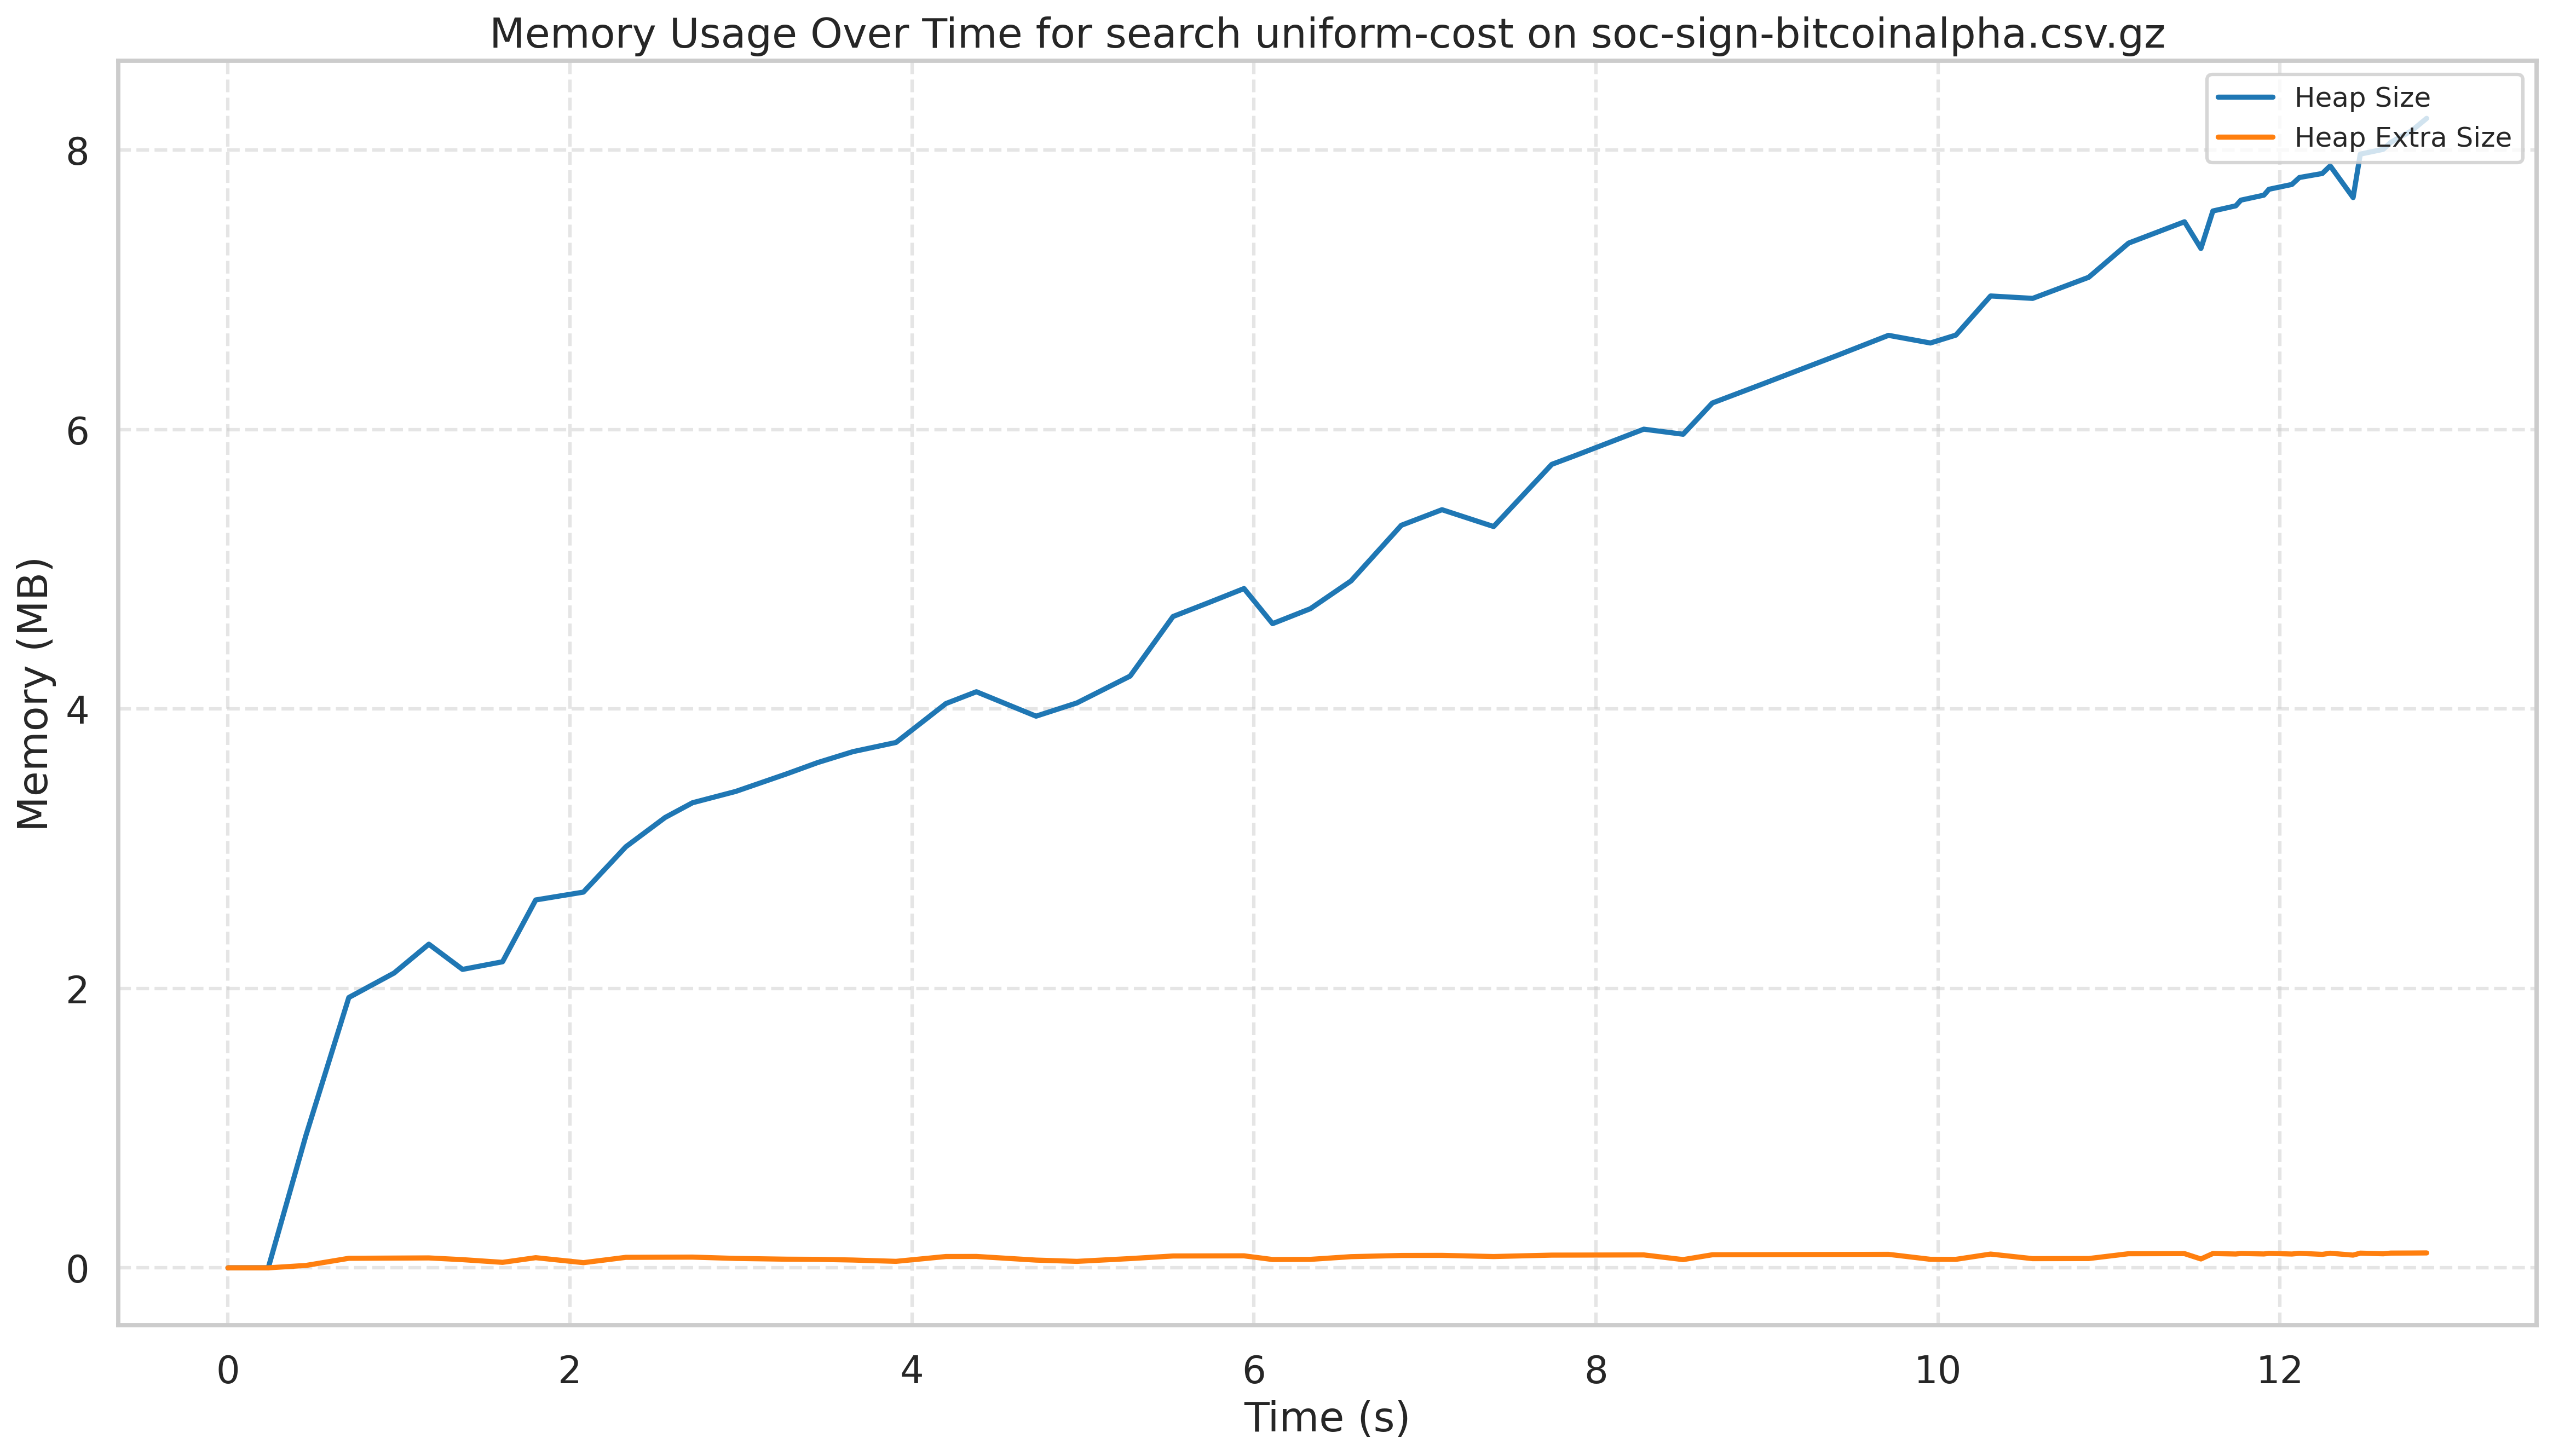
\includegraphics[width=\textwidth]{../plots/soc-sign-bitcoinalpha.csv_uniform-cost.png}
\caption{Grafico: breadth-first su com-lj.ungraph}
\end{figure}
\subsubsection{Algoritmo di ricerca: depth-limited}
\begin{figure}[h]\centering
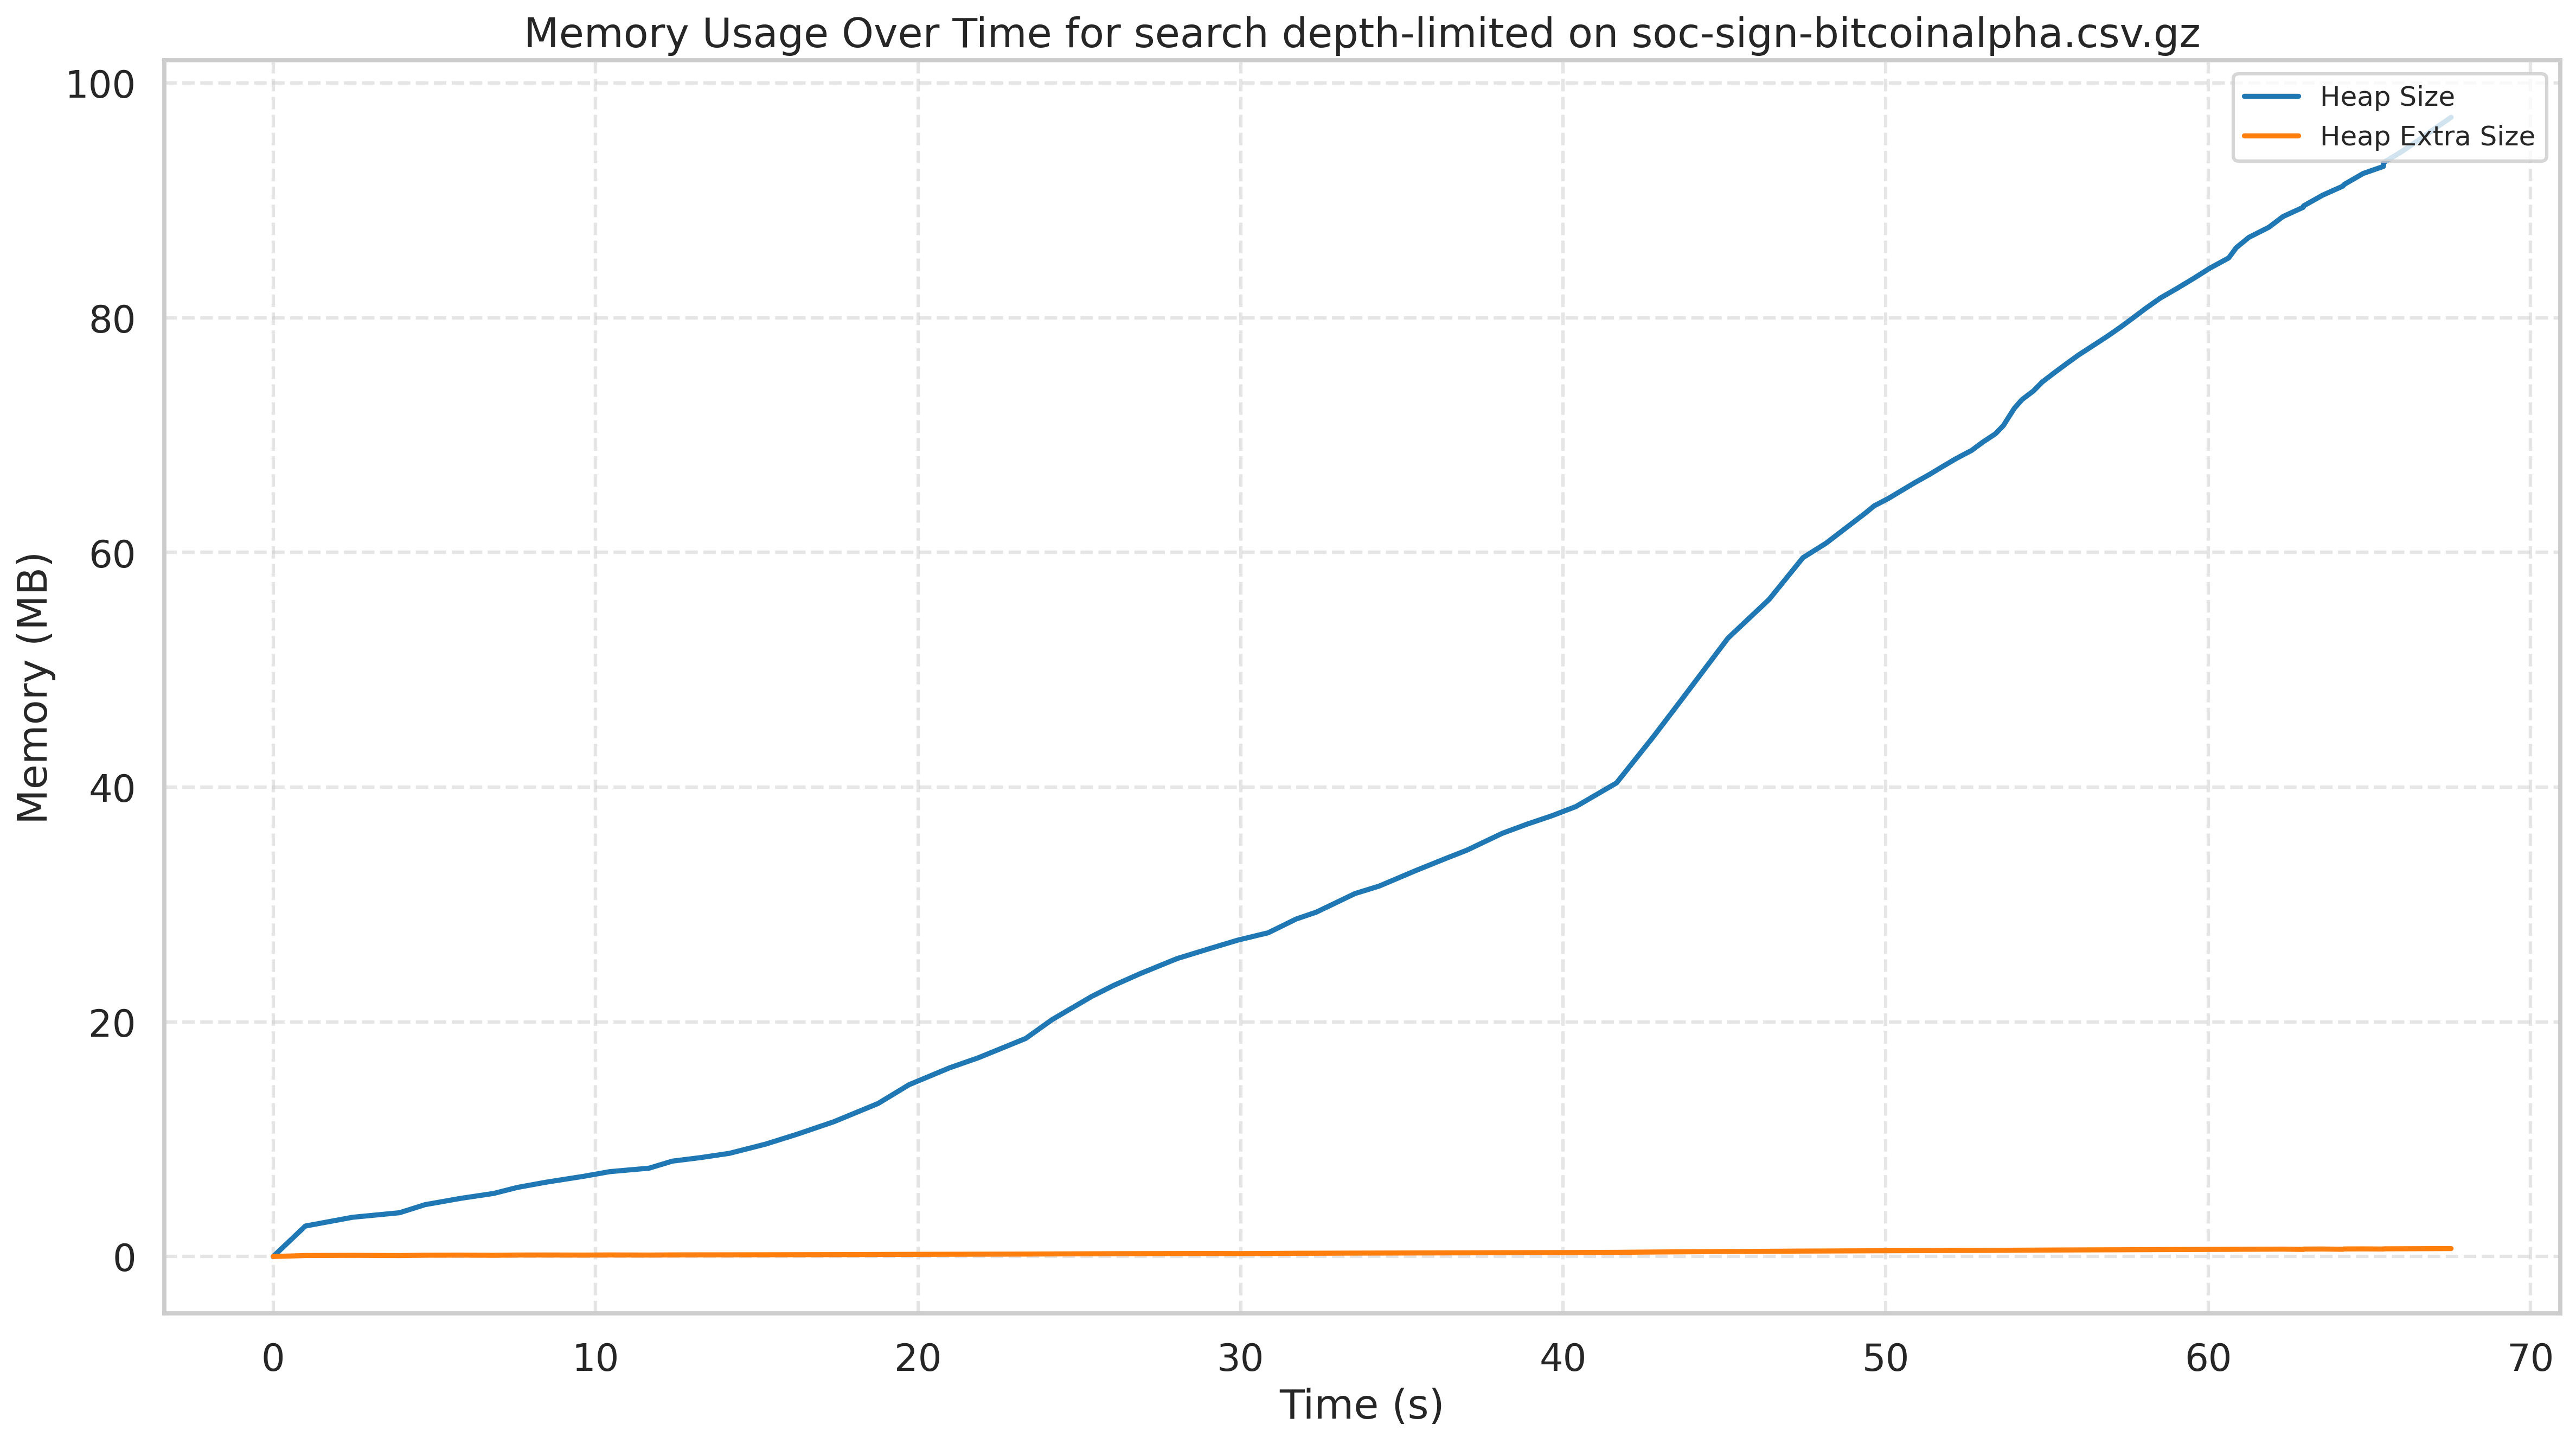
\includegraphics[width=\textwidth]{../plots/soc-sign-bitcoinalpha.csv_depth-limited.png}
\caption{Grafico: breadth-first su com-lj.ungraph}
\end{figure}
\subsubsection{Algoritmo di ricerca: iterative-deepening}
\begin{figure}[h]\centering
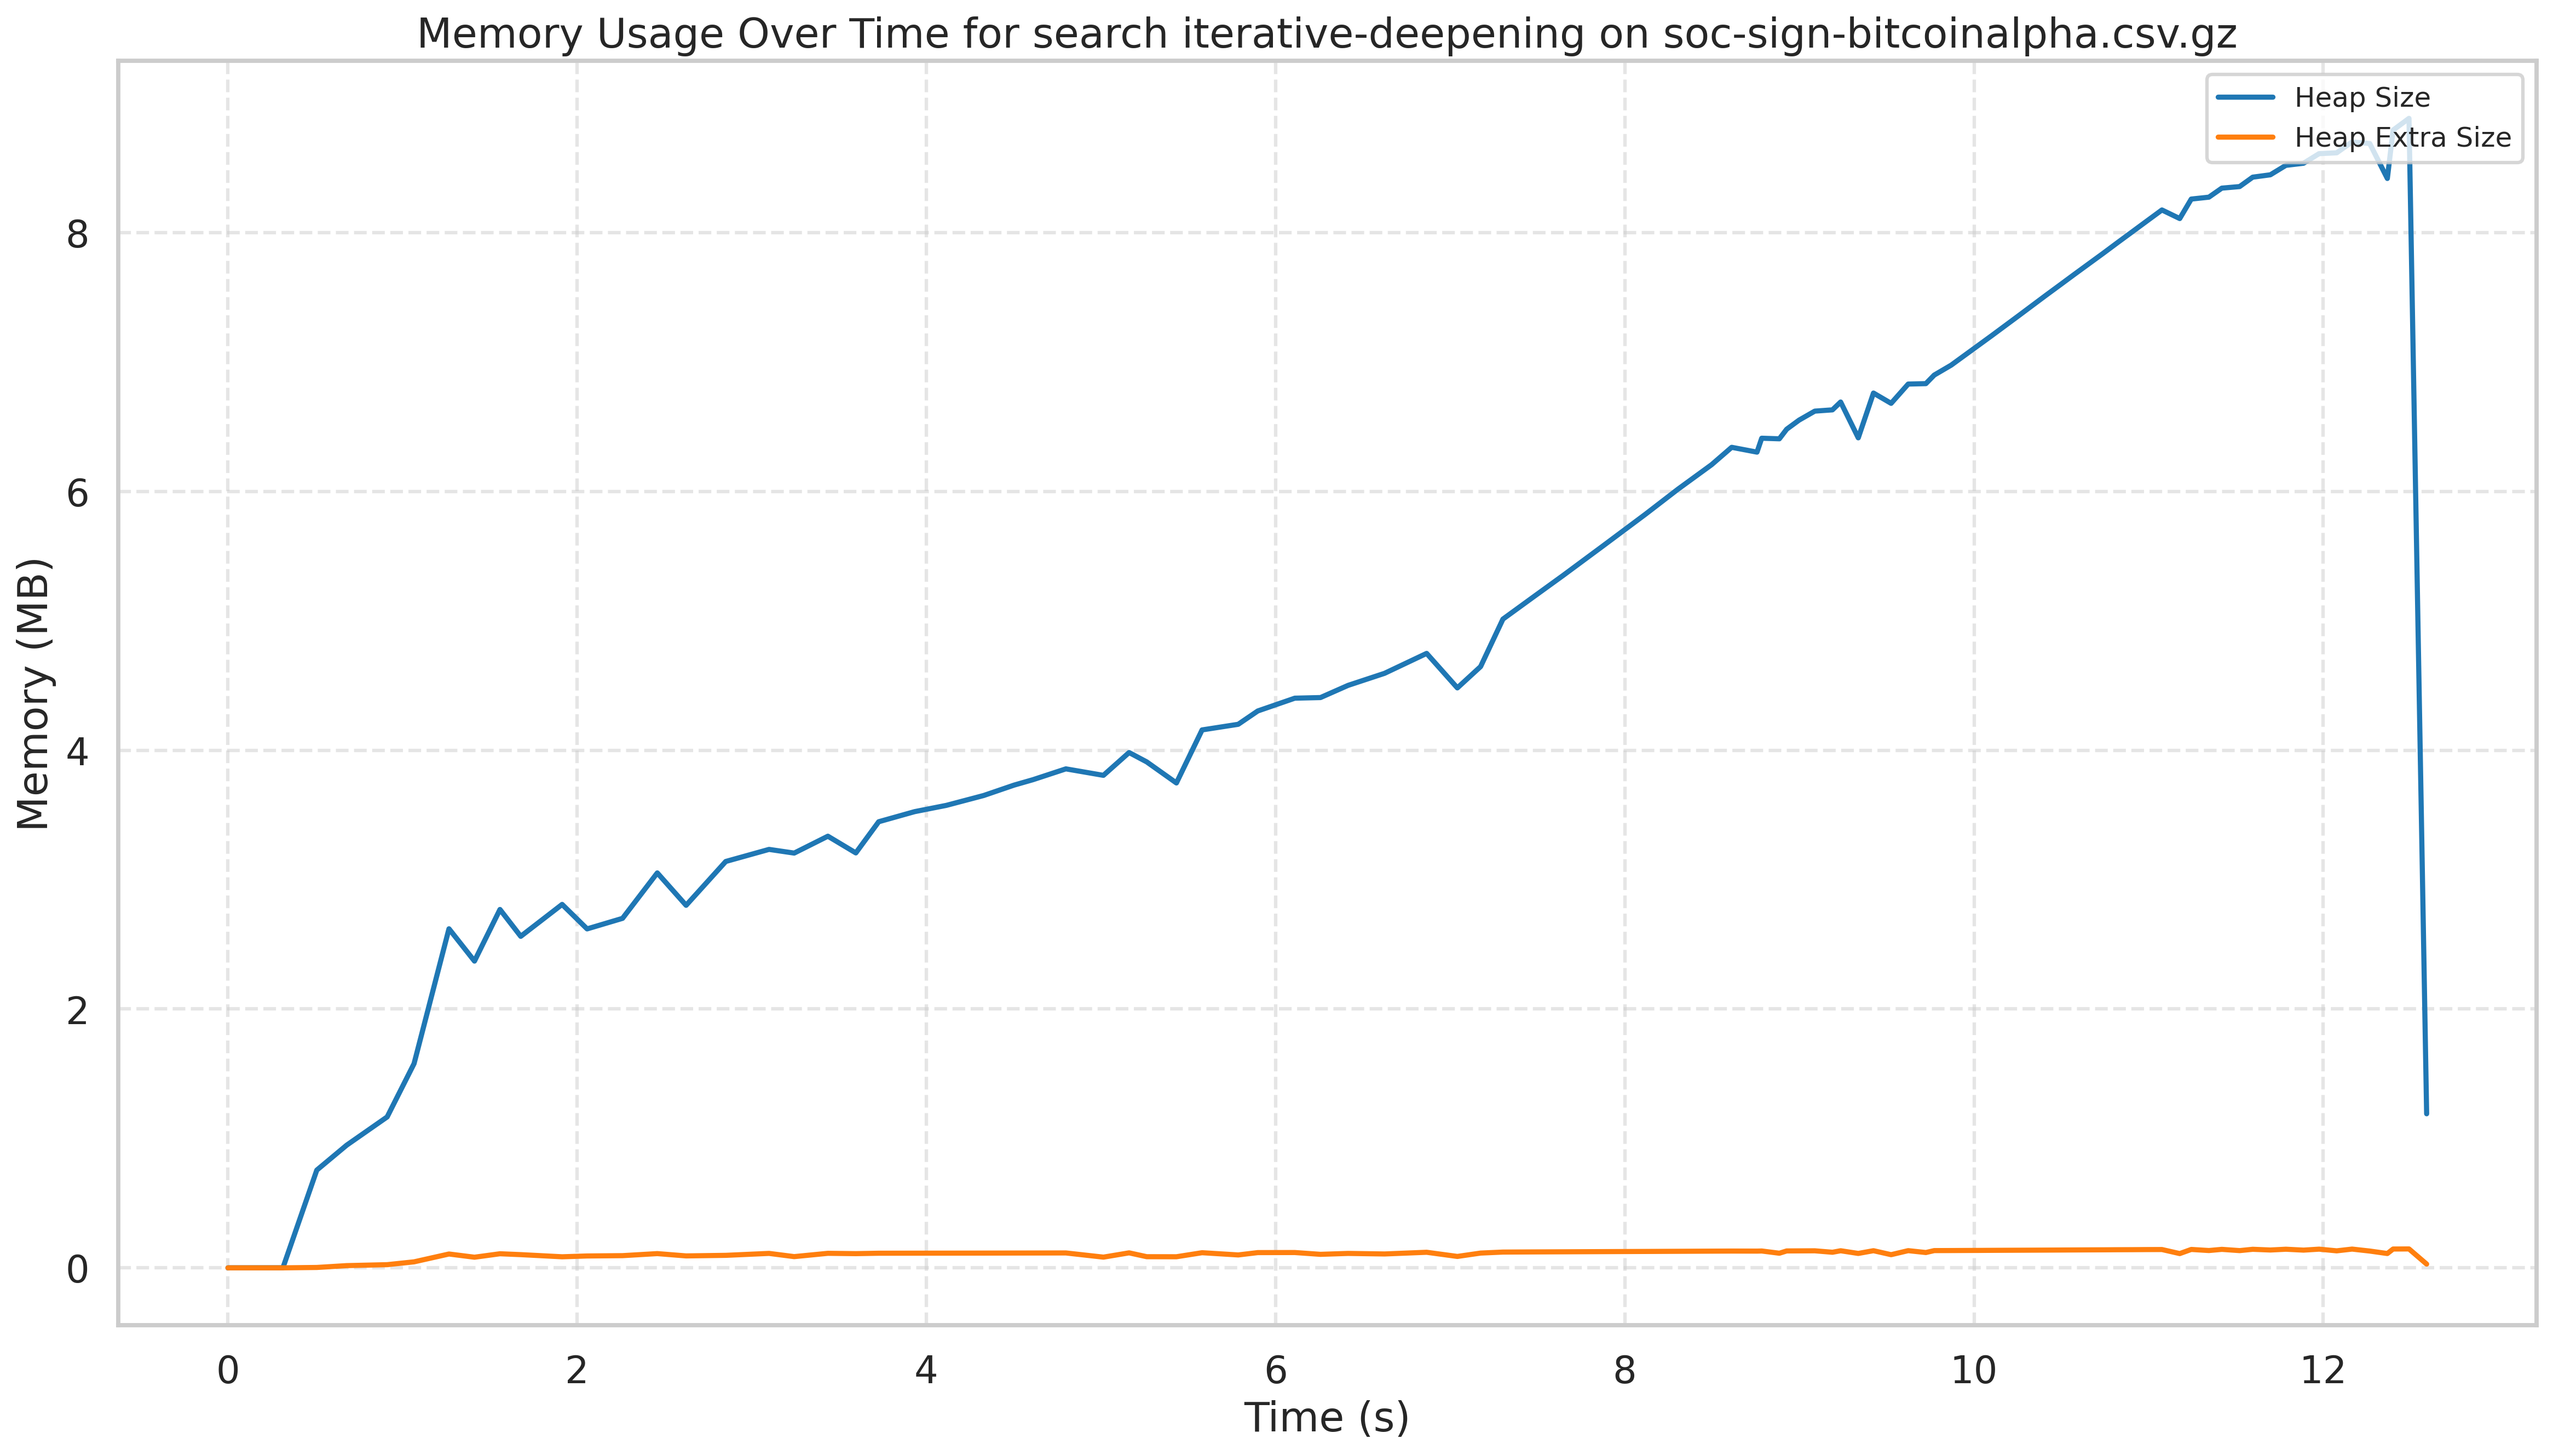
\includegraphics[width=\textwidth]{../plots/soc-sign-bitcoinalpha.csv_iterative-deepening.png}
\caption{Grafico: breadth-first su com-lj.ungraph}
\end{figure}
\subsubsection{Algoritmo di ricerca: bi-directional}
\begin{figure}[h]\centering
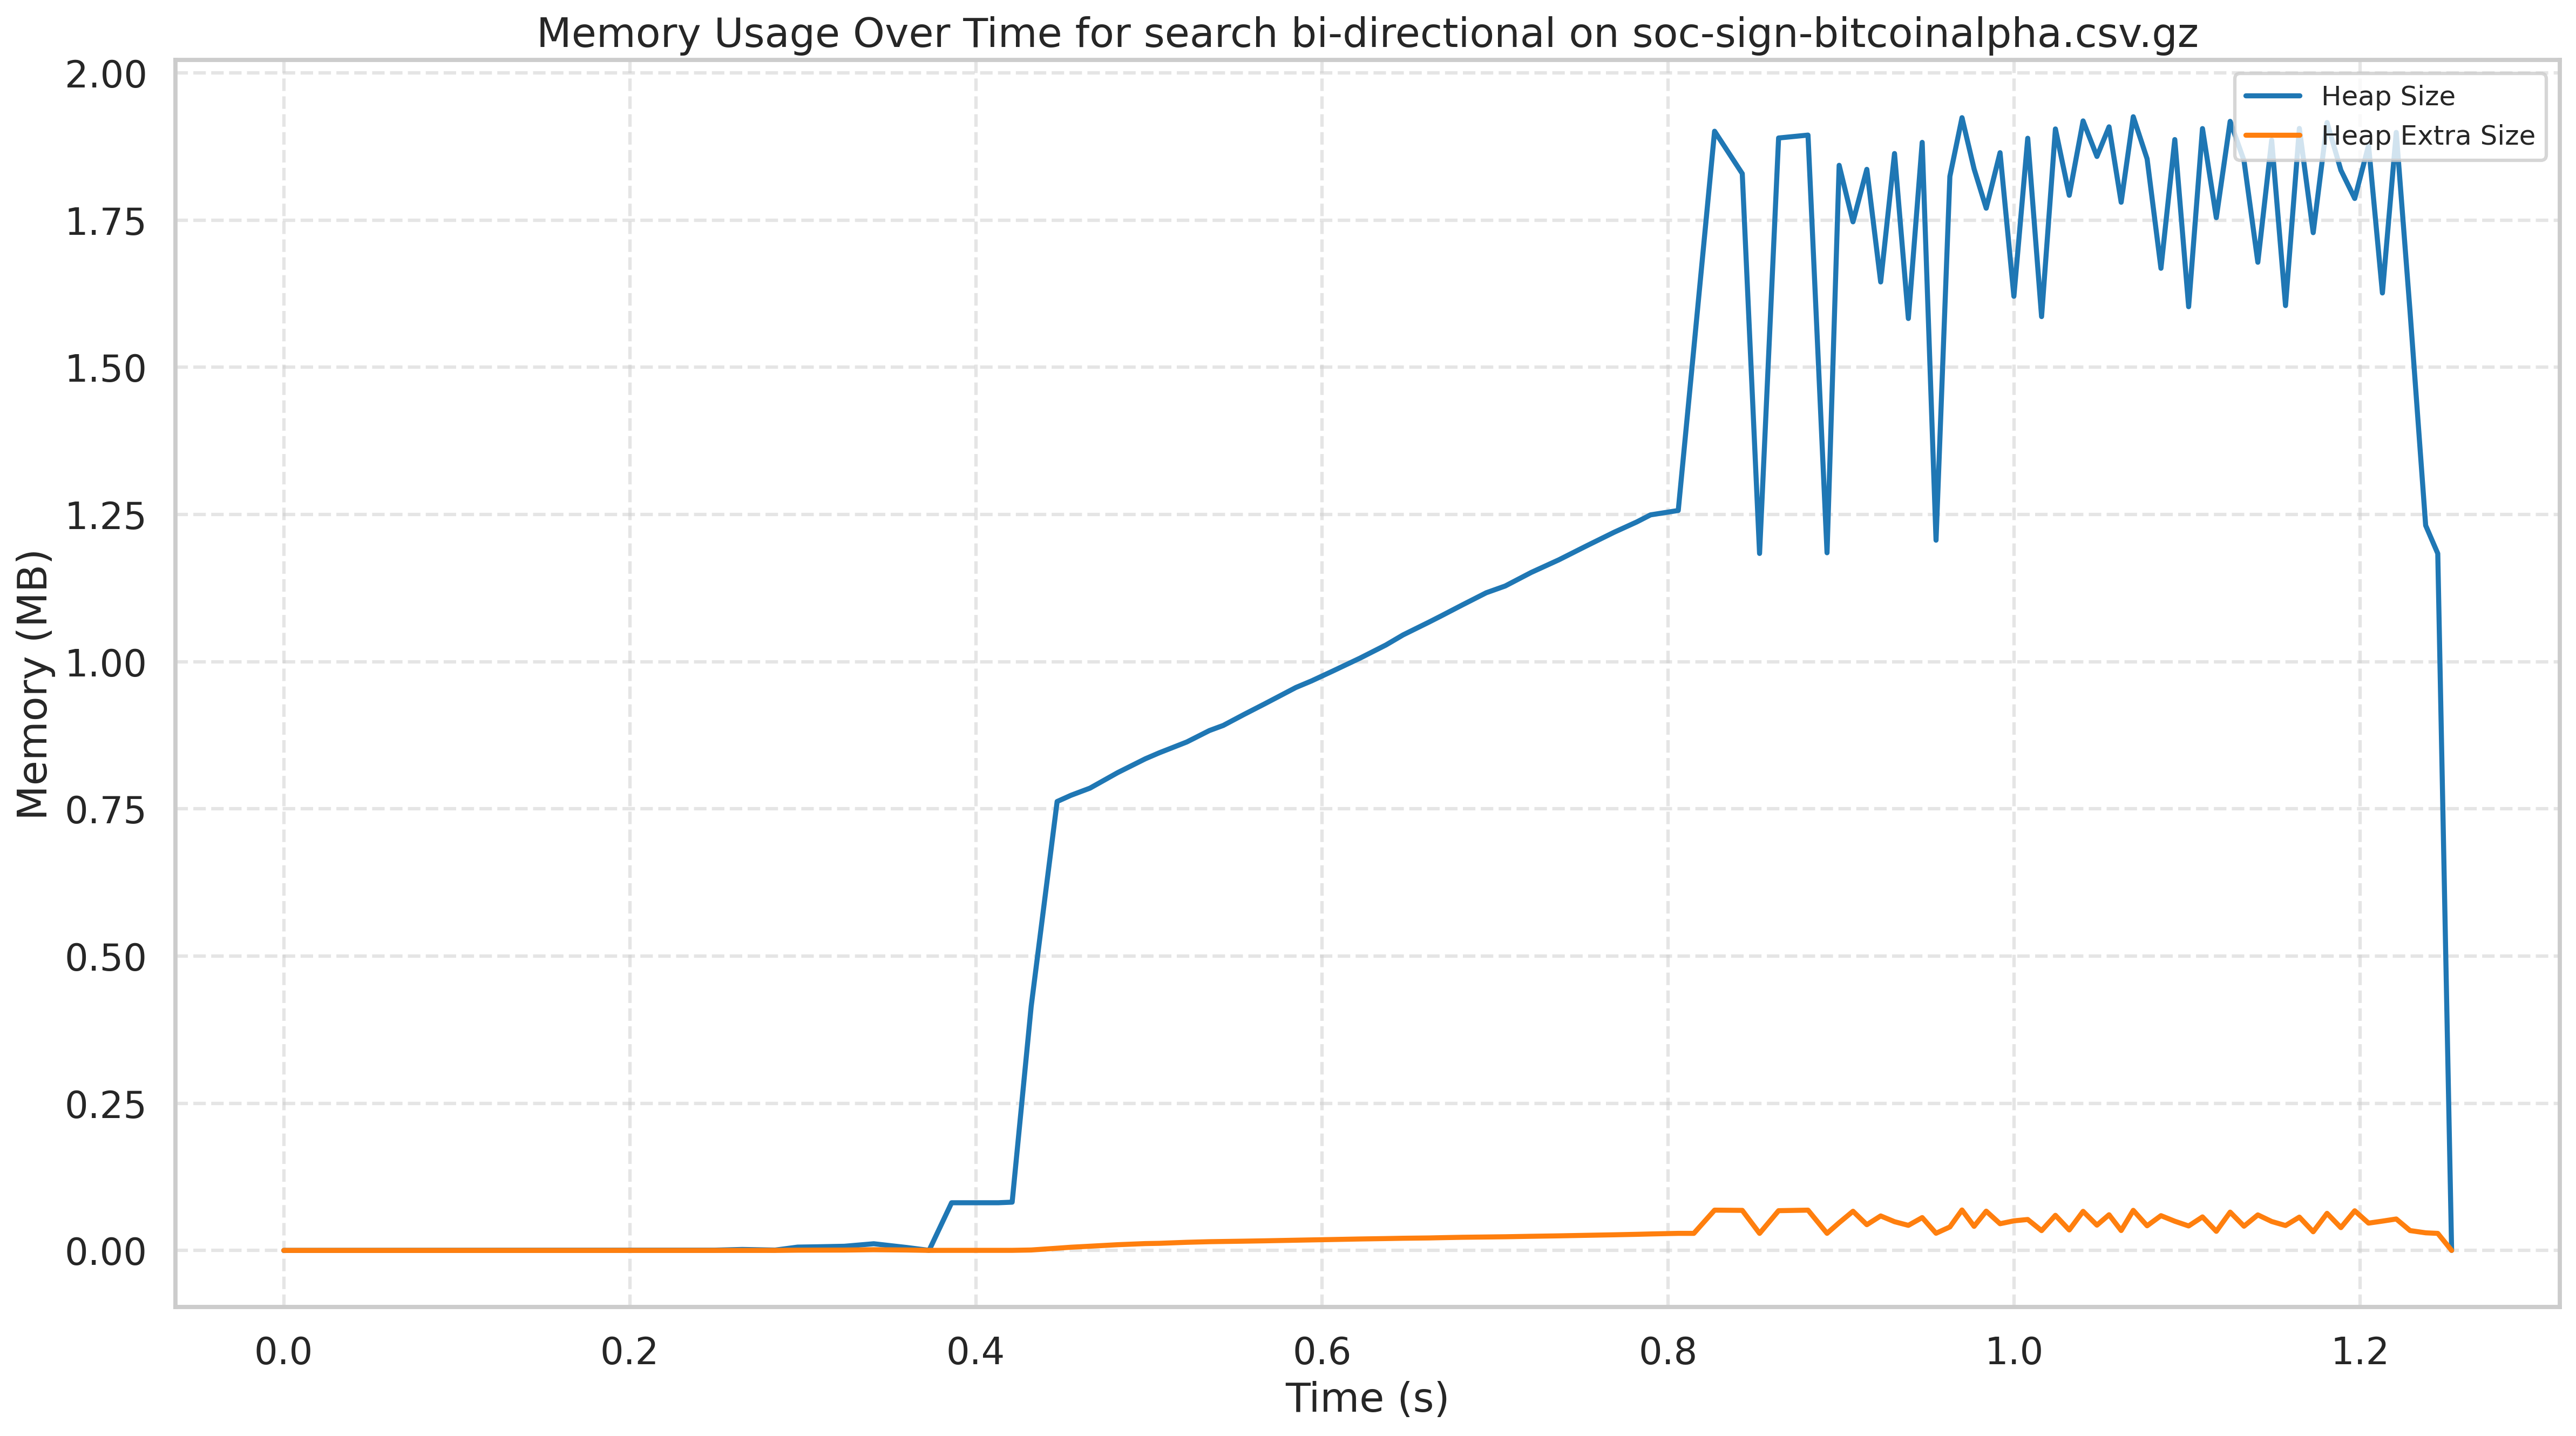
\includegraphics[width=\textwidth]{../plots/soc-sign-bitcoinalpha.csv_bi-directional.png}
\caption{Grafico: breadth-first su com-lj.ungraph}
\end{figure}
\subsubsection{Algoritmo di ricerca: breadth-first}
\begin{figure}[h]\centering
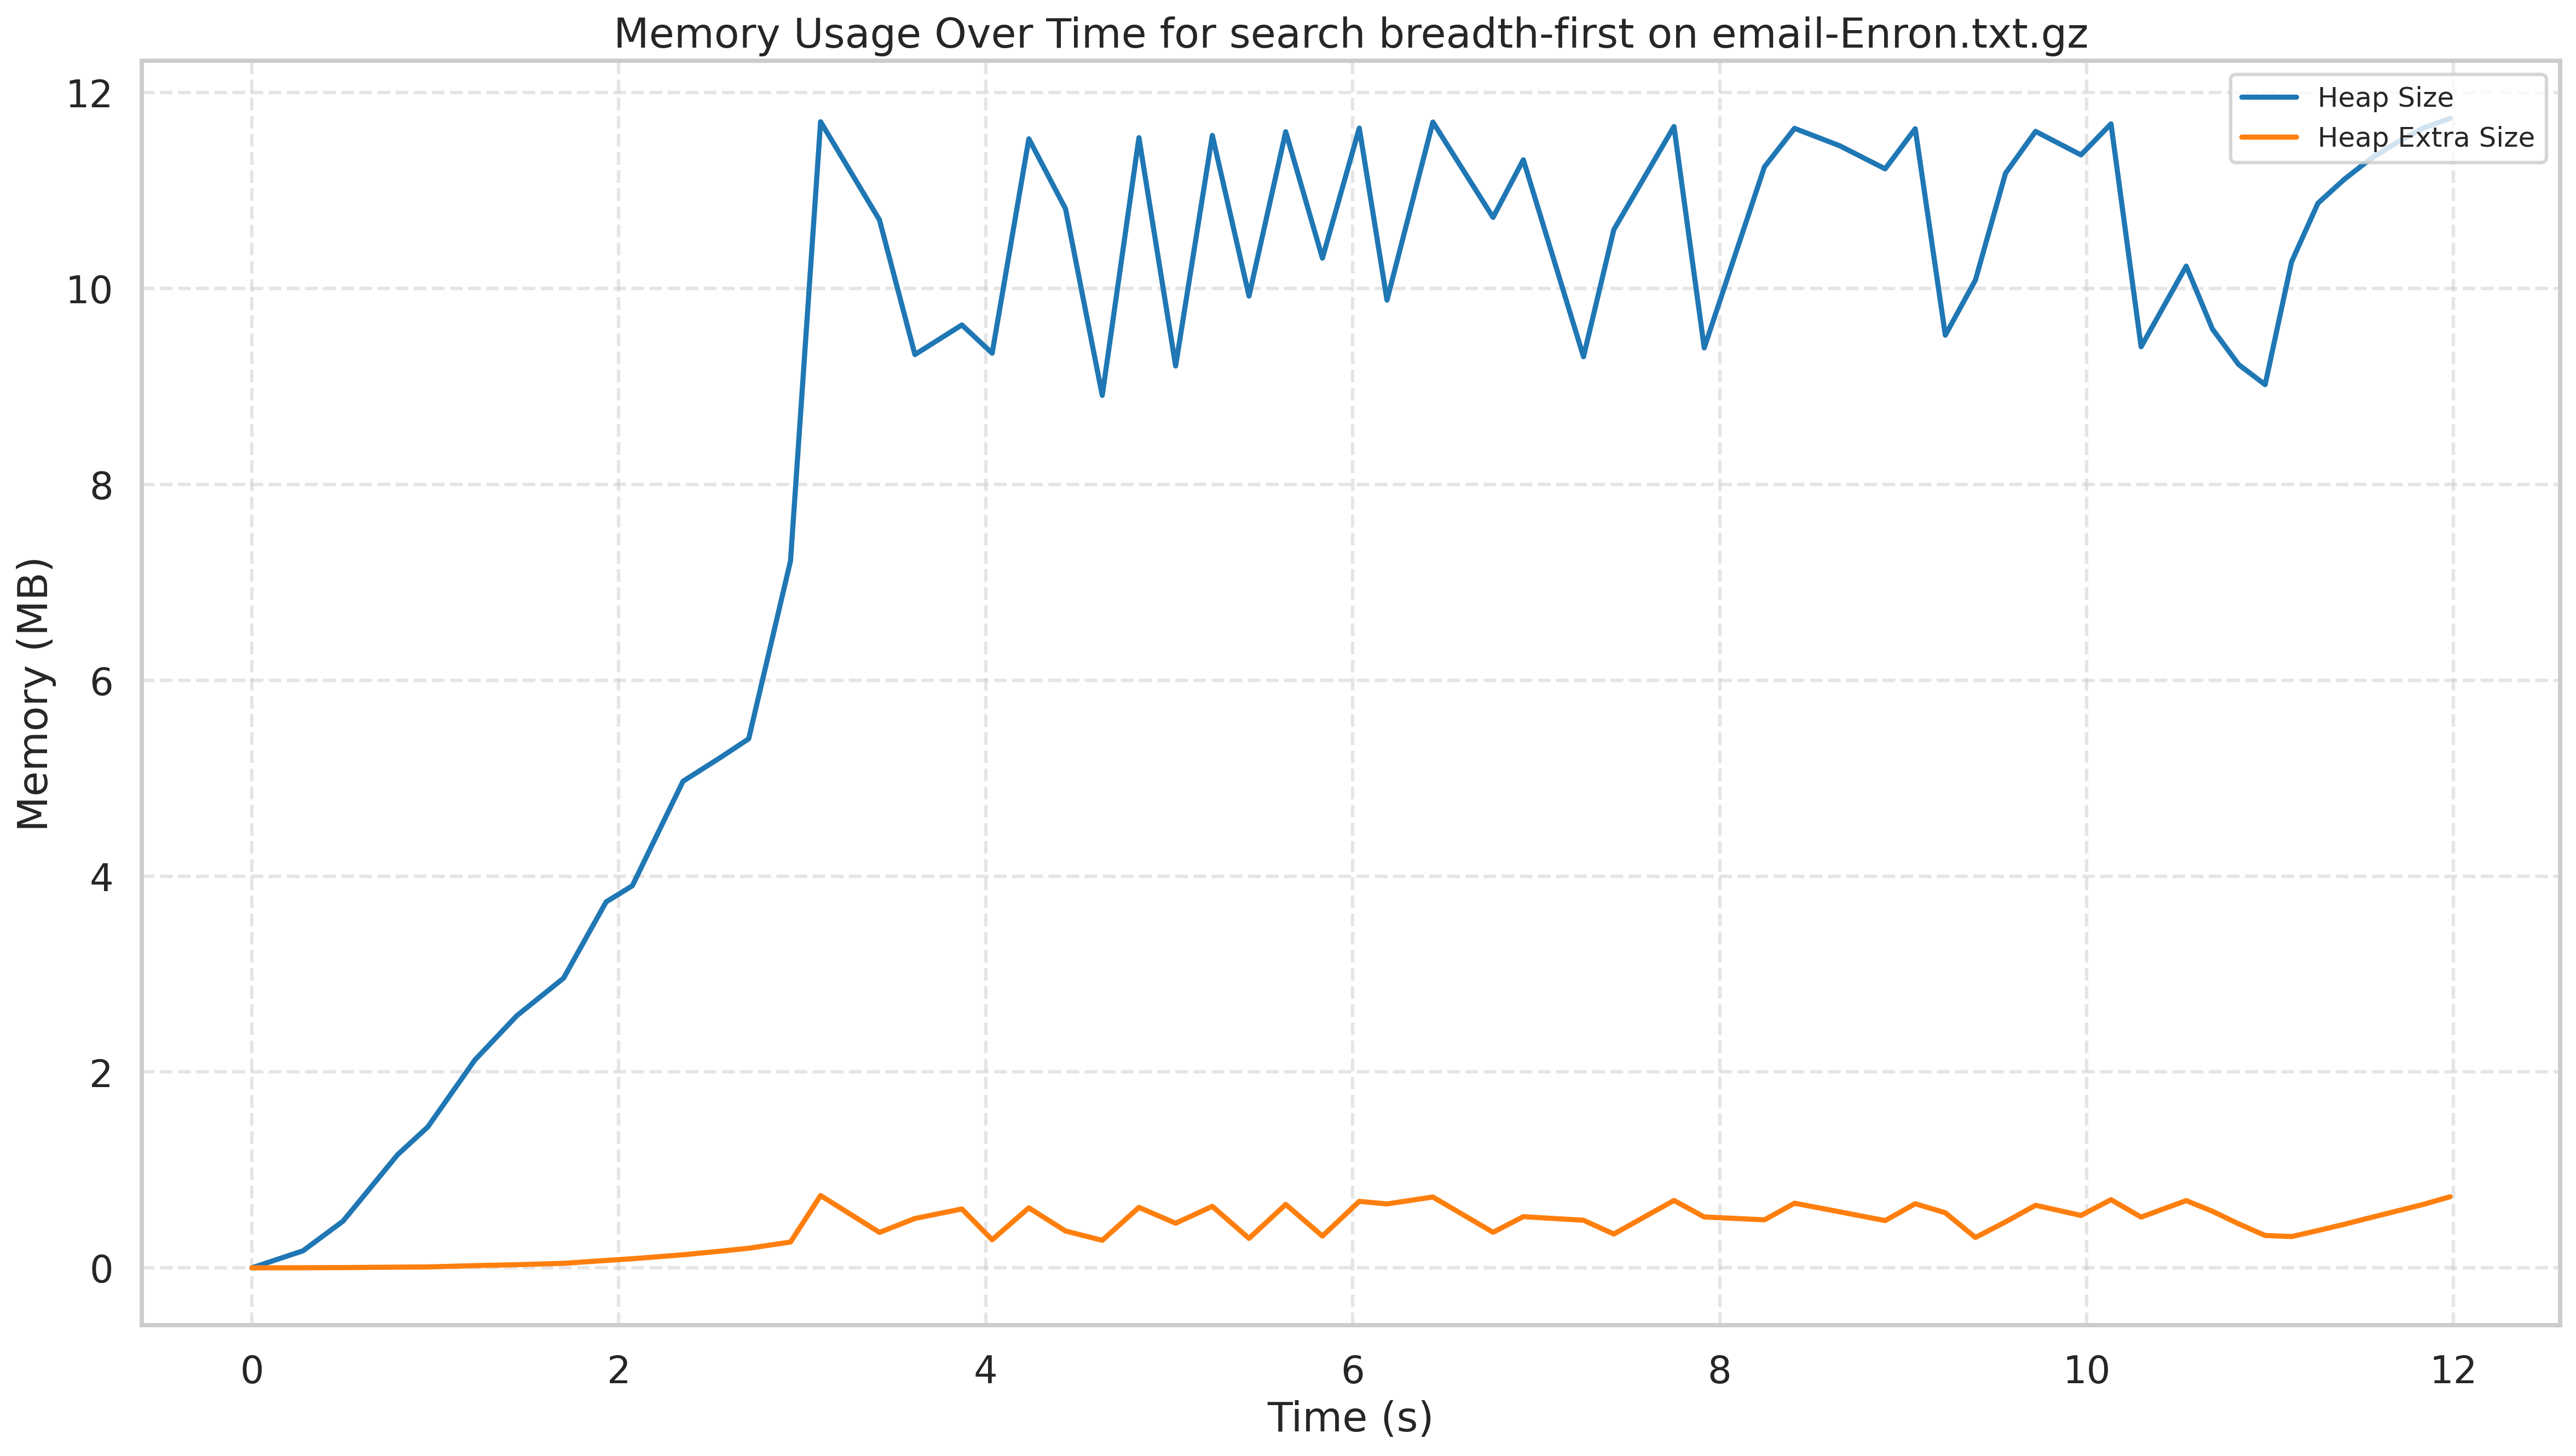
\includegraphics[width=\textwidth]{../plots/email-Enron_breadth-first.png}
\caption{Grafico: breadth-first su com-lj.ungraph}
\end{figure}
\subsubsection{Algoritmo di ricerca: uniform-cost}
\begin{figure}[h]\centering
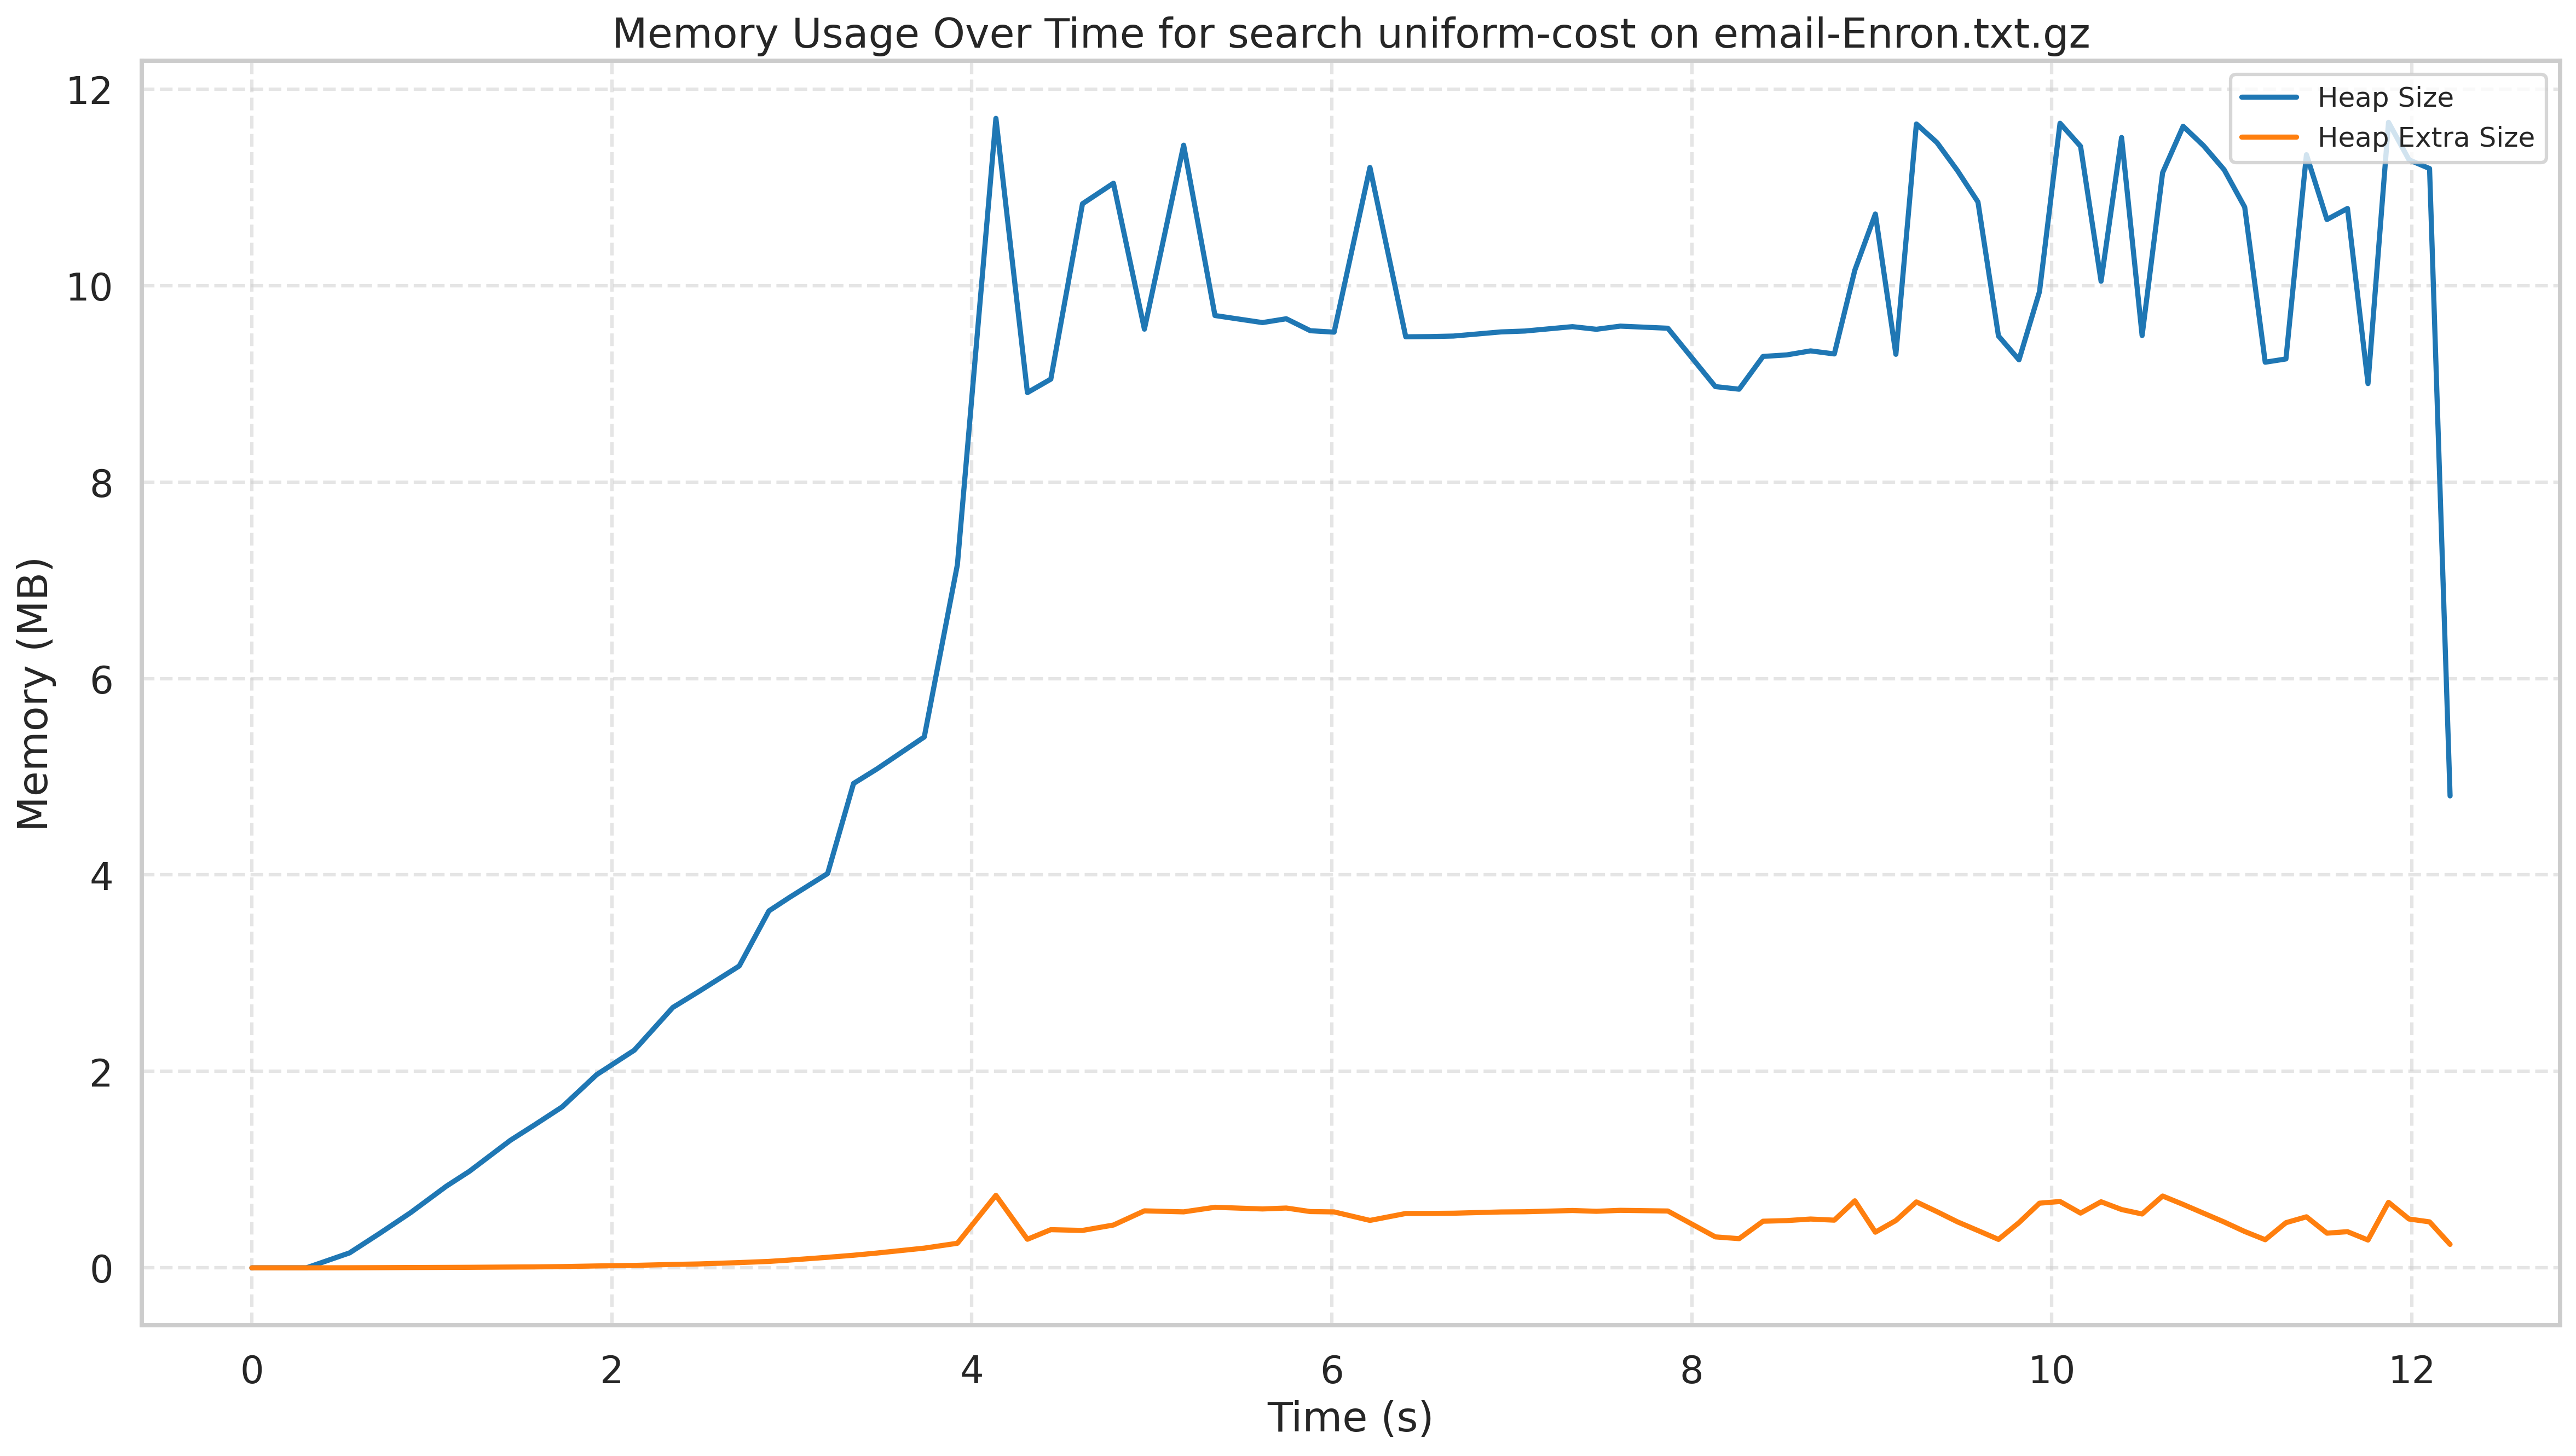
\includegraphics[width=\textwidth]{../plots/email-Enron_uniform-cost.png}
\caption{Grafico: breadth-first su com-lj.ungraph}
\end{figure}
\subsubsection{Algoritmo di ricerca: depth-limited}
\begin{figure}[h]\centering
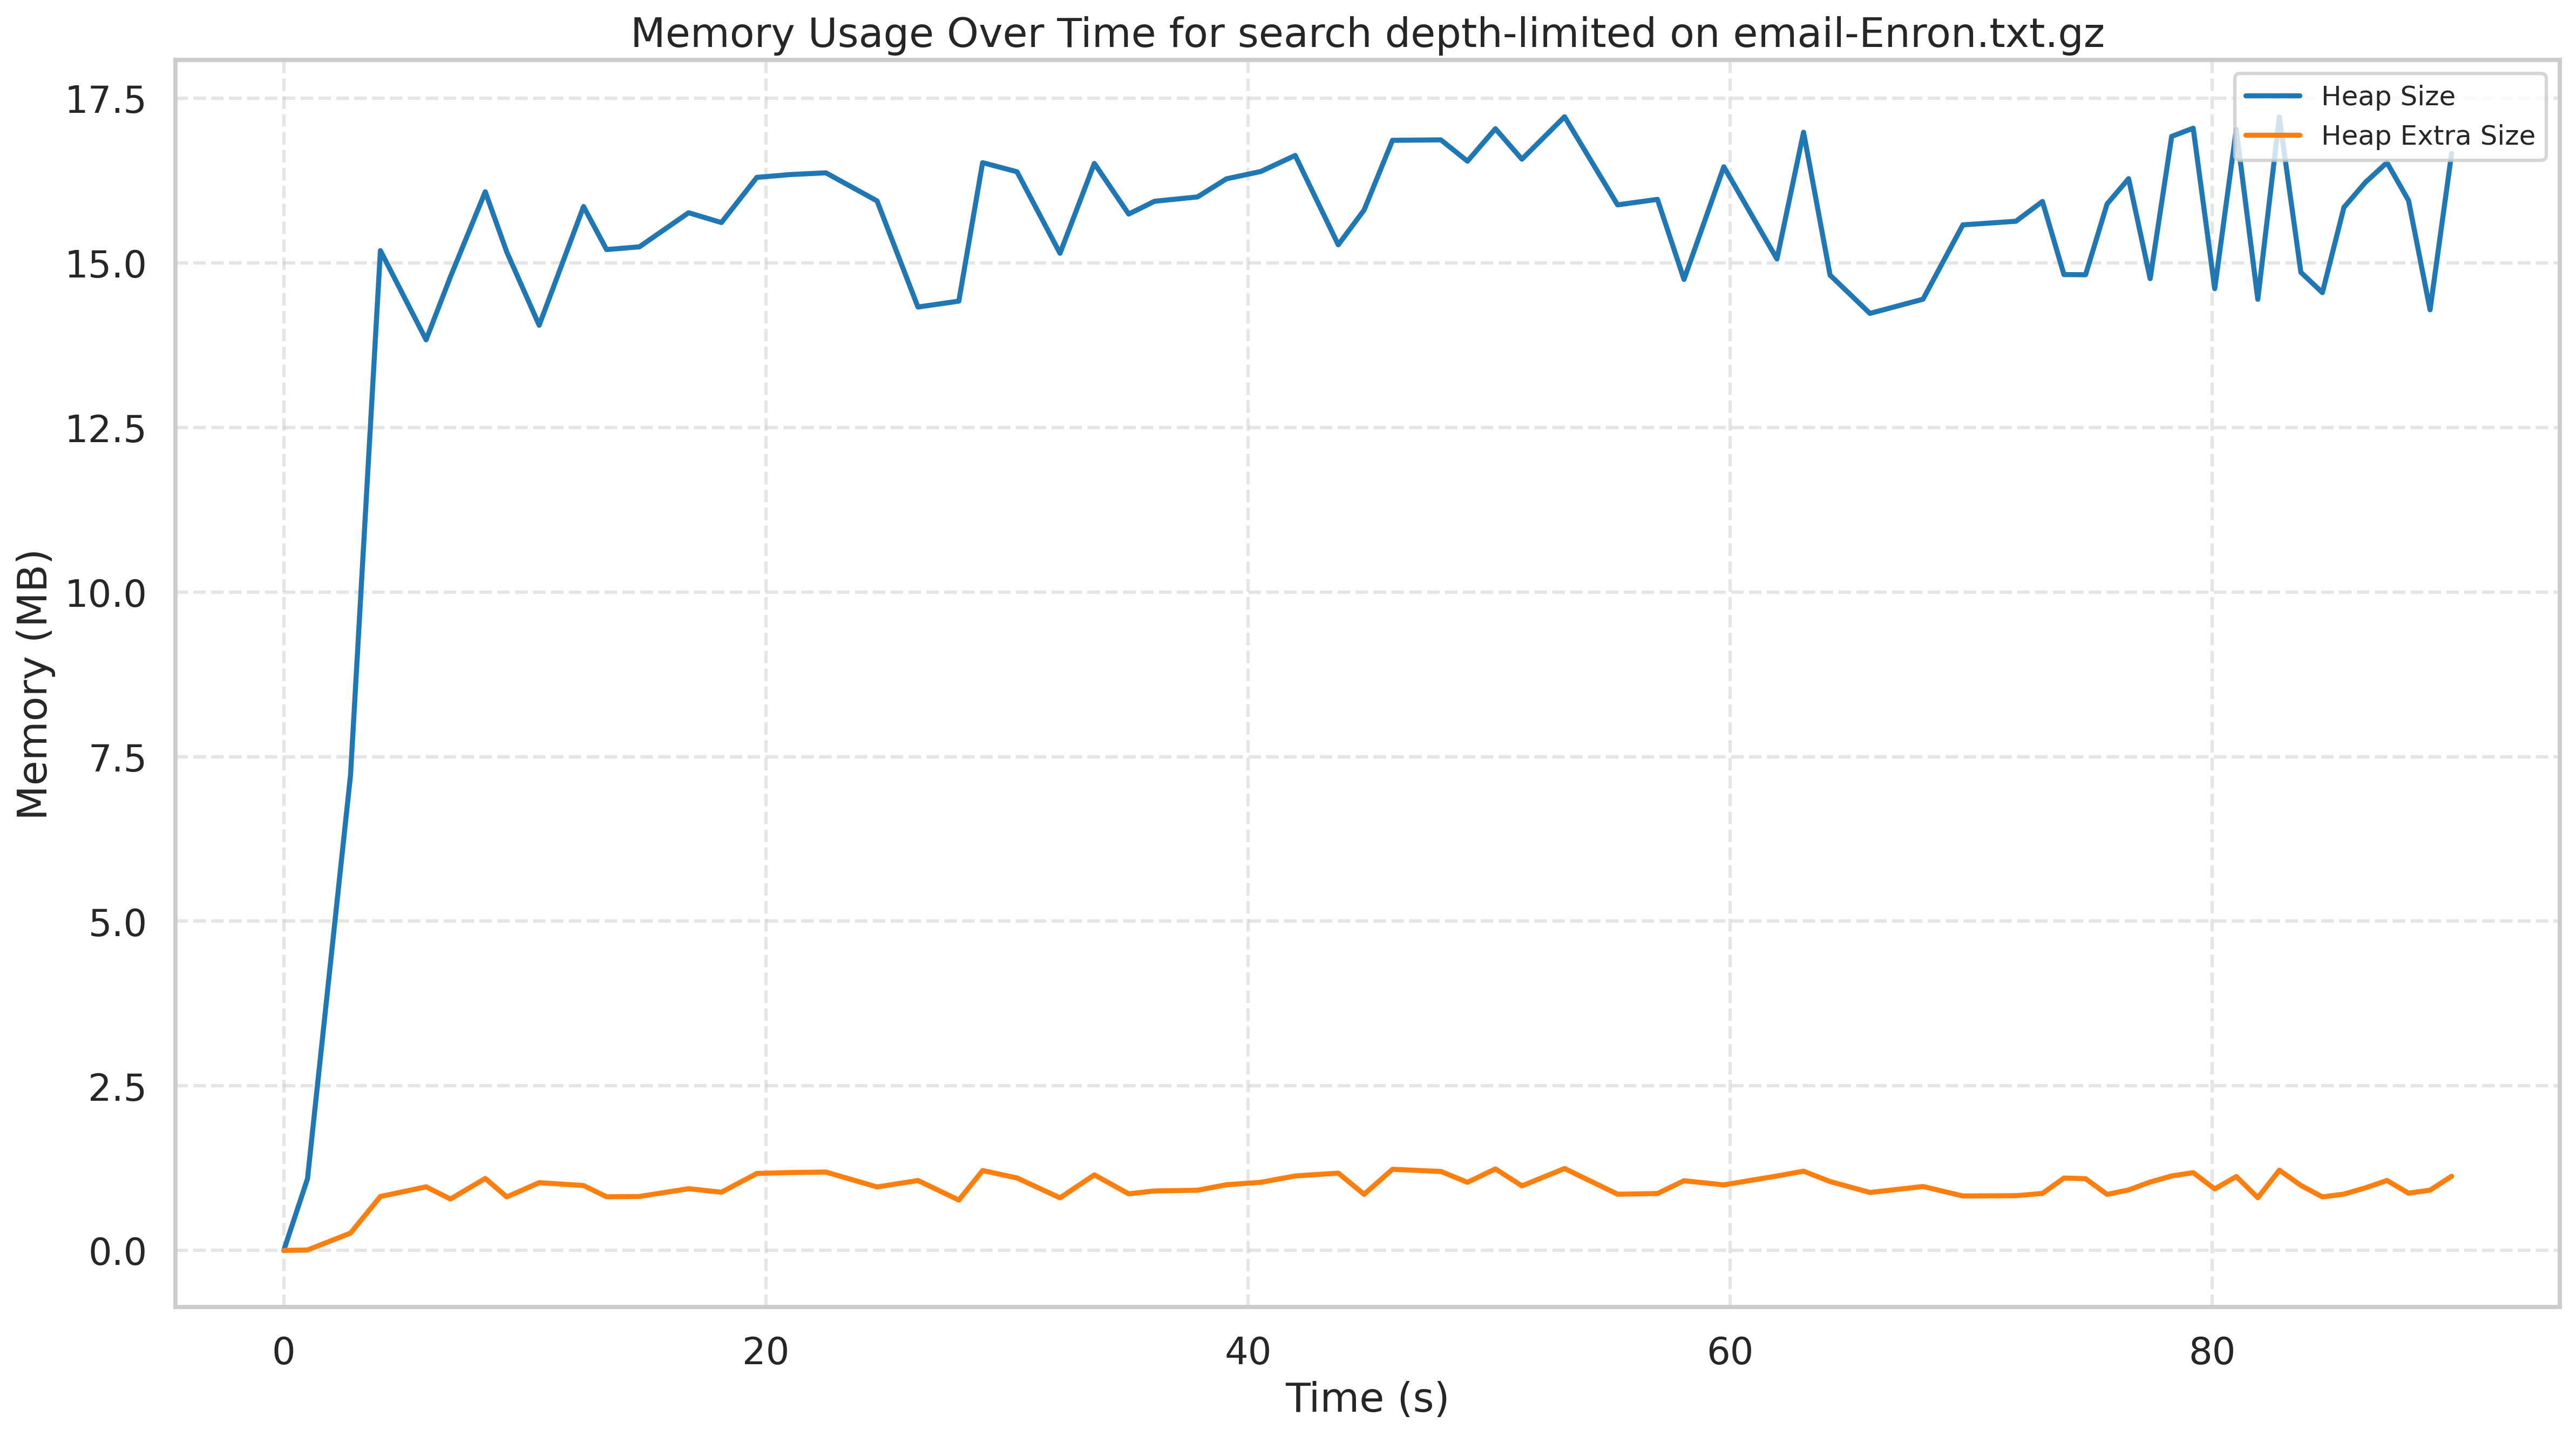
\includegraphics[width=\textwidth]{../plots/email-Enron_depth-limited.png}
\caption{Grafico: breadth-first su com-lj.ungraph}
\end{figure}
\subsubsection{Algoritmo di ricerca: iterative-deepening}
\begin{figure}[h]\centering
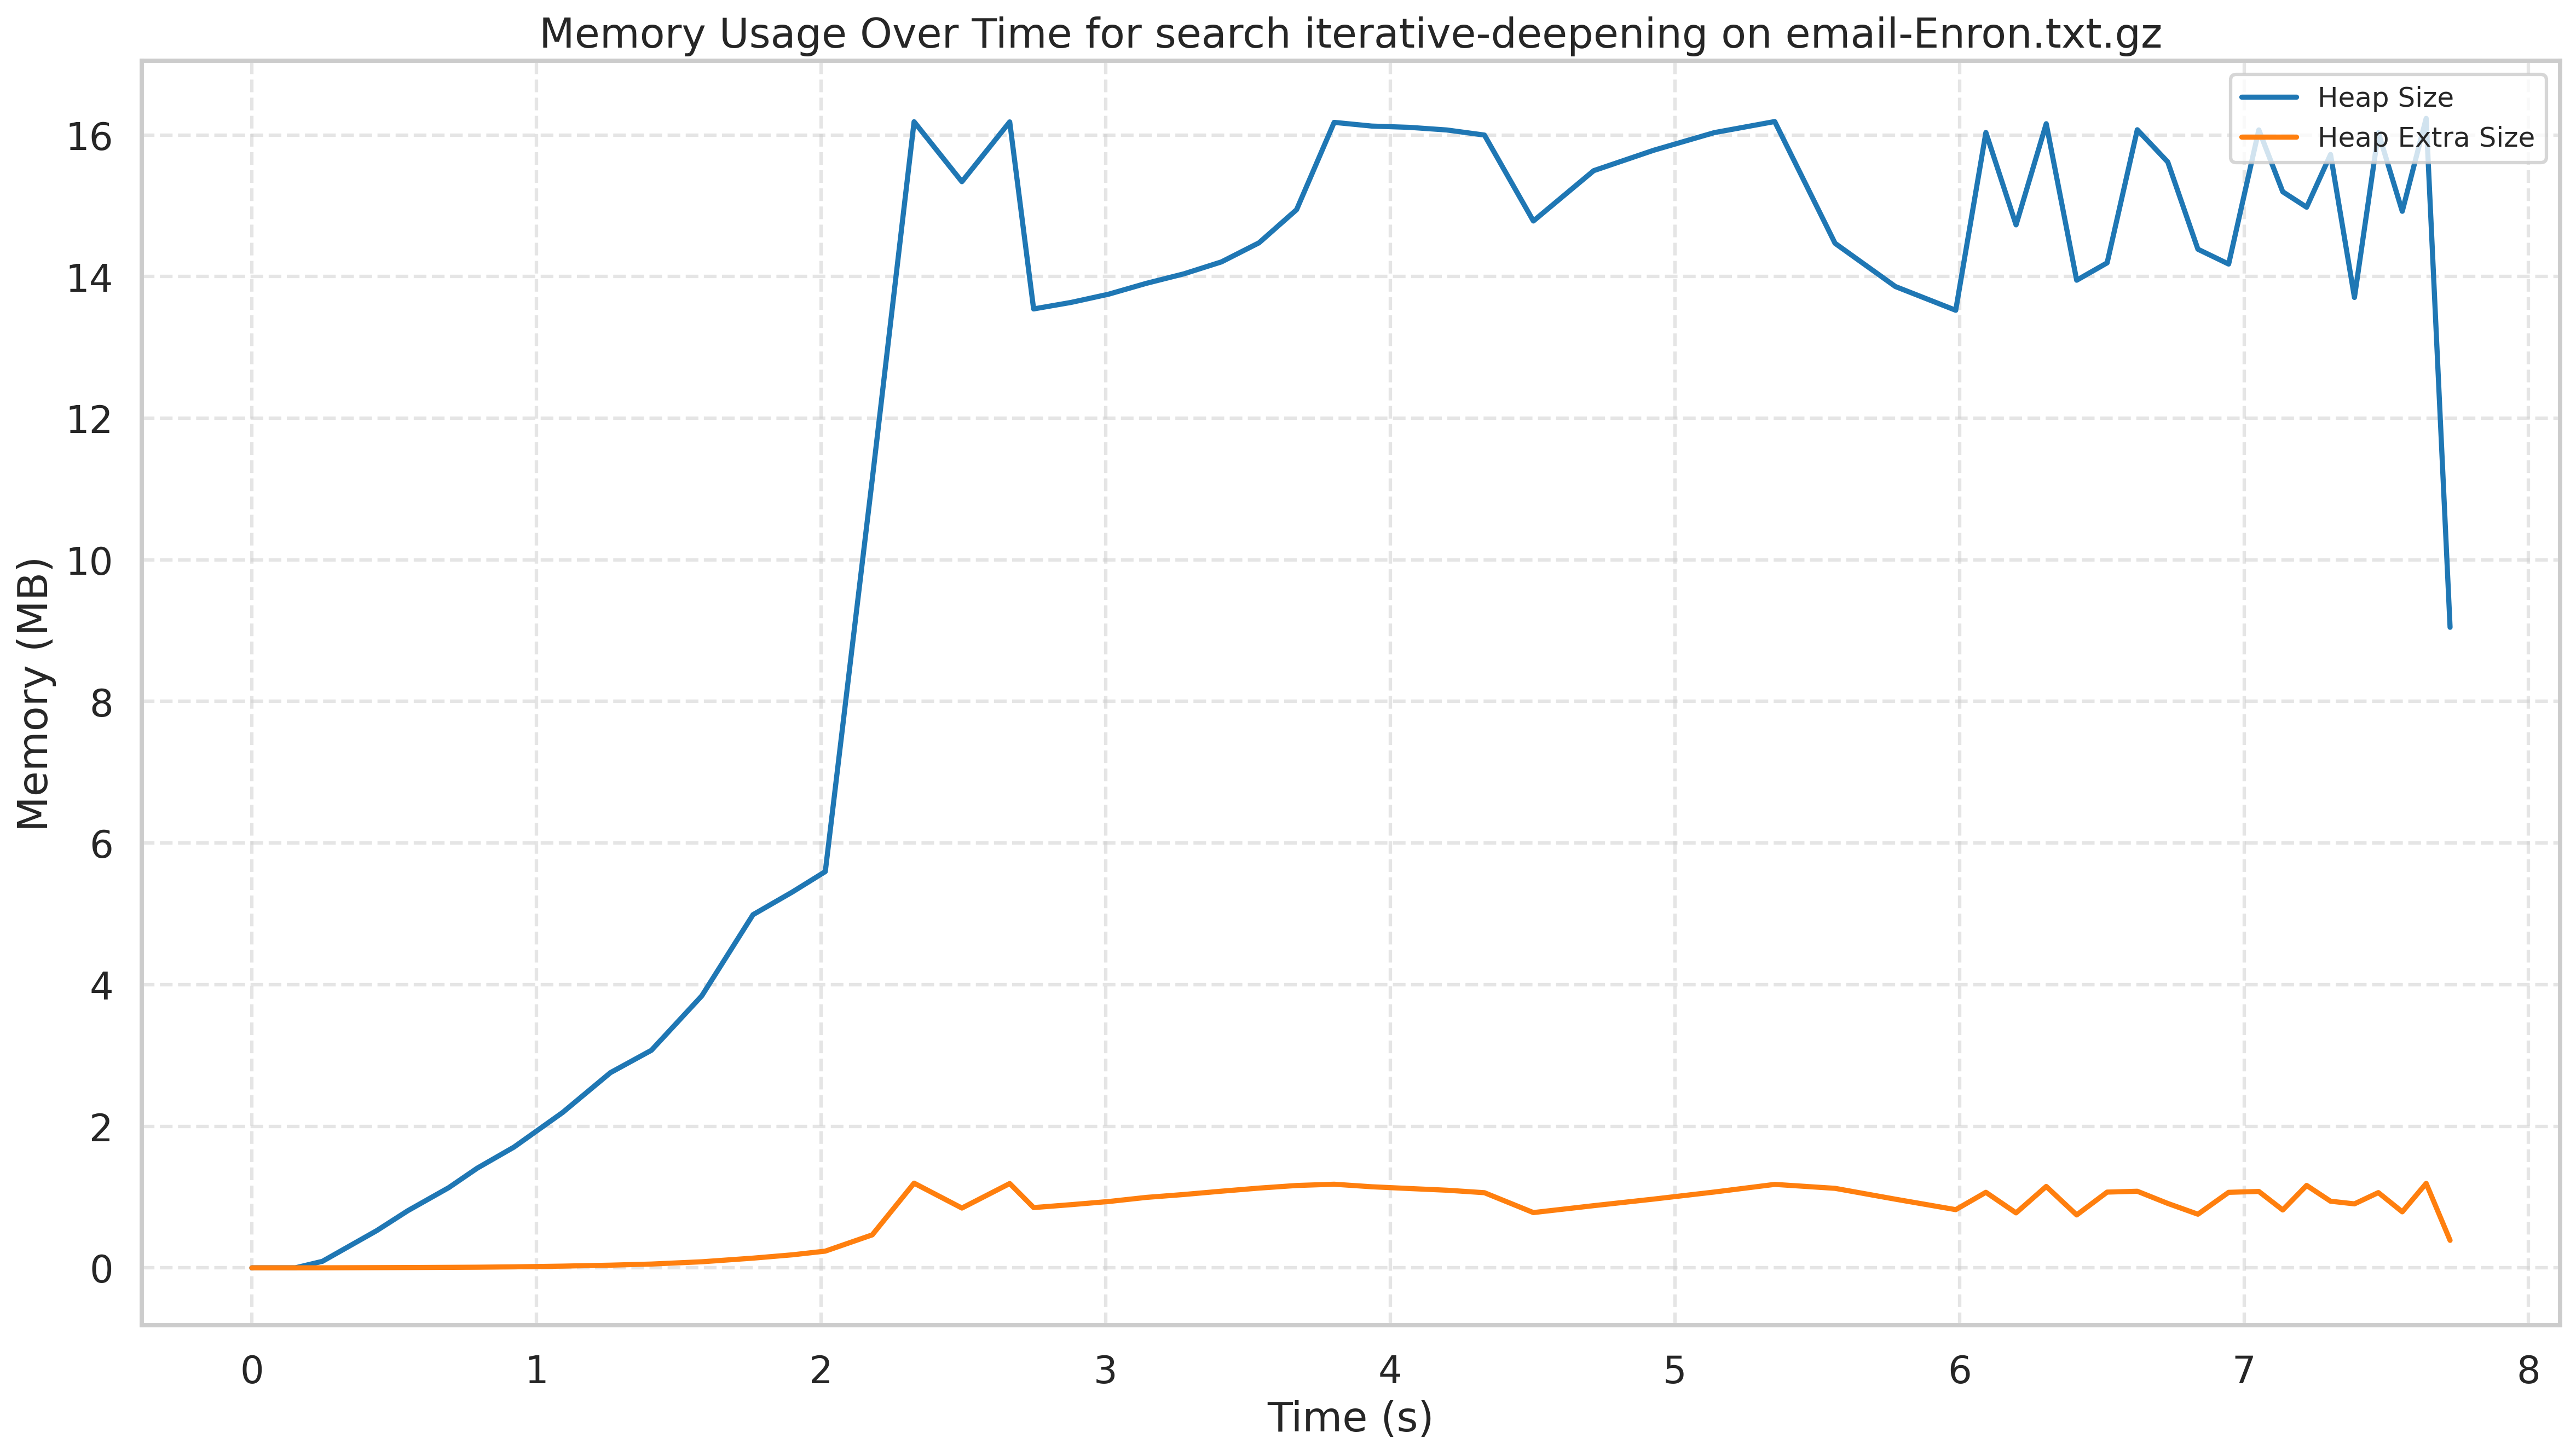
\includegraphics[width=\textwidth]{../plots/email-Enron_iterative-deepening.png}
\caption{Grafico: breadth-first su com-lj.ungraph}
\end{figure}
\subsubsection{Algoritmo di ricerca: bi-directional}
\begin{figure}[h]\centering
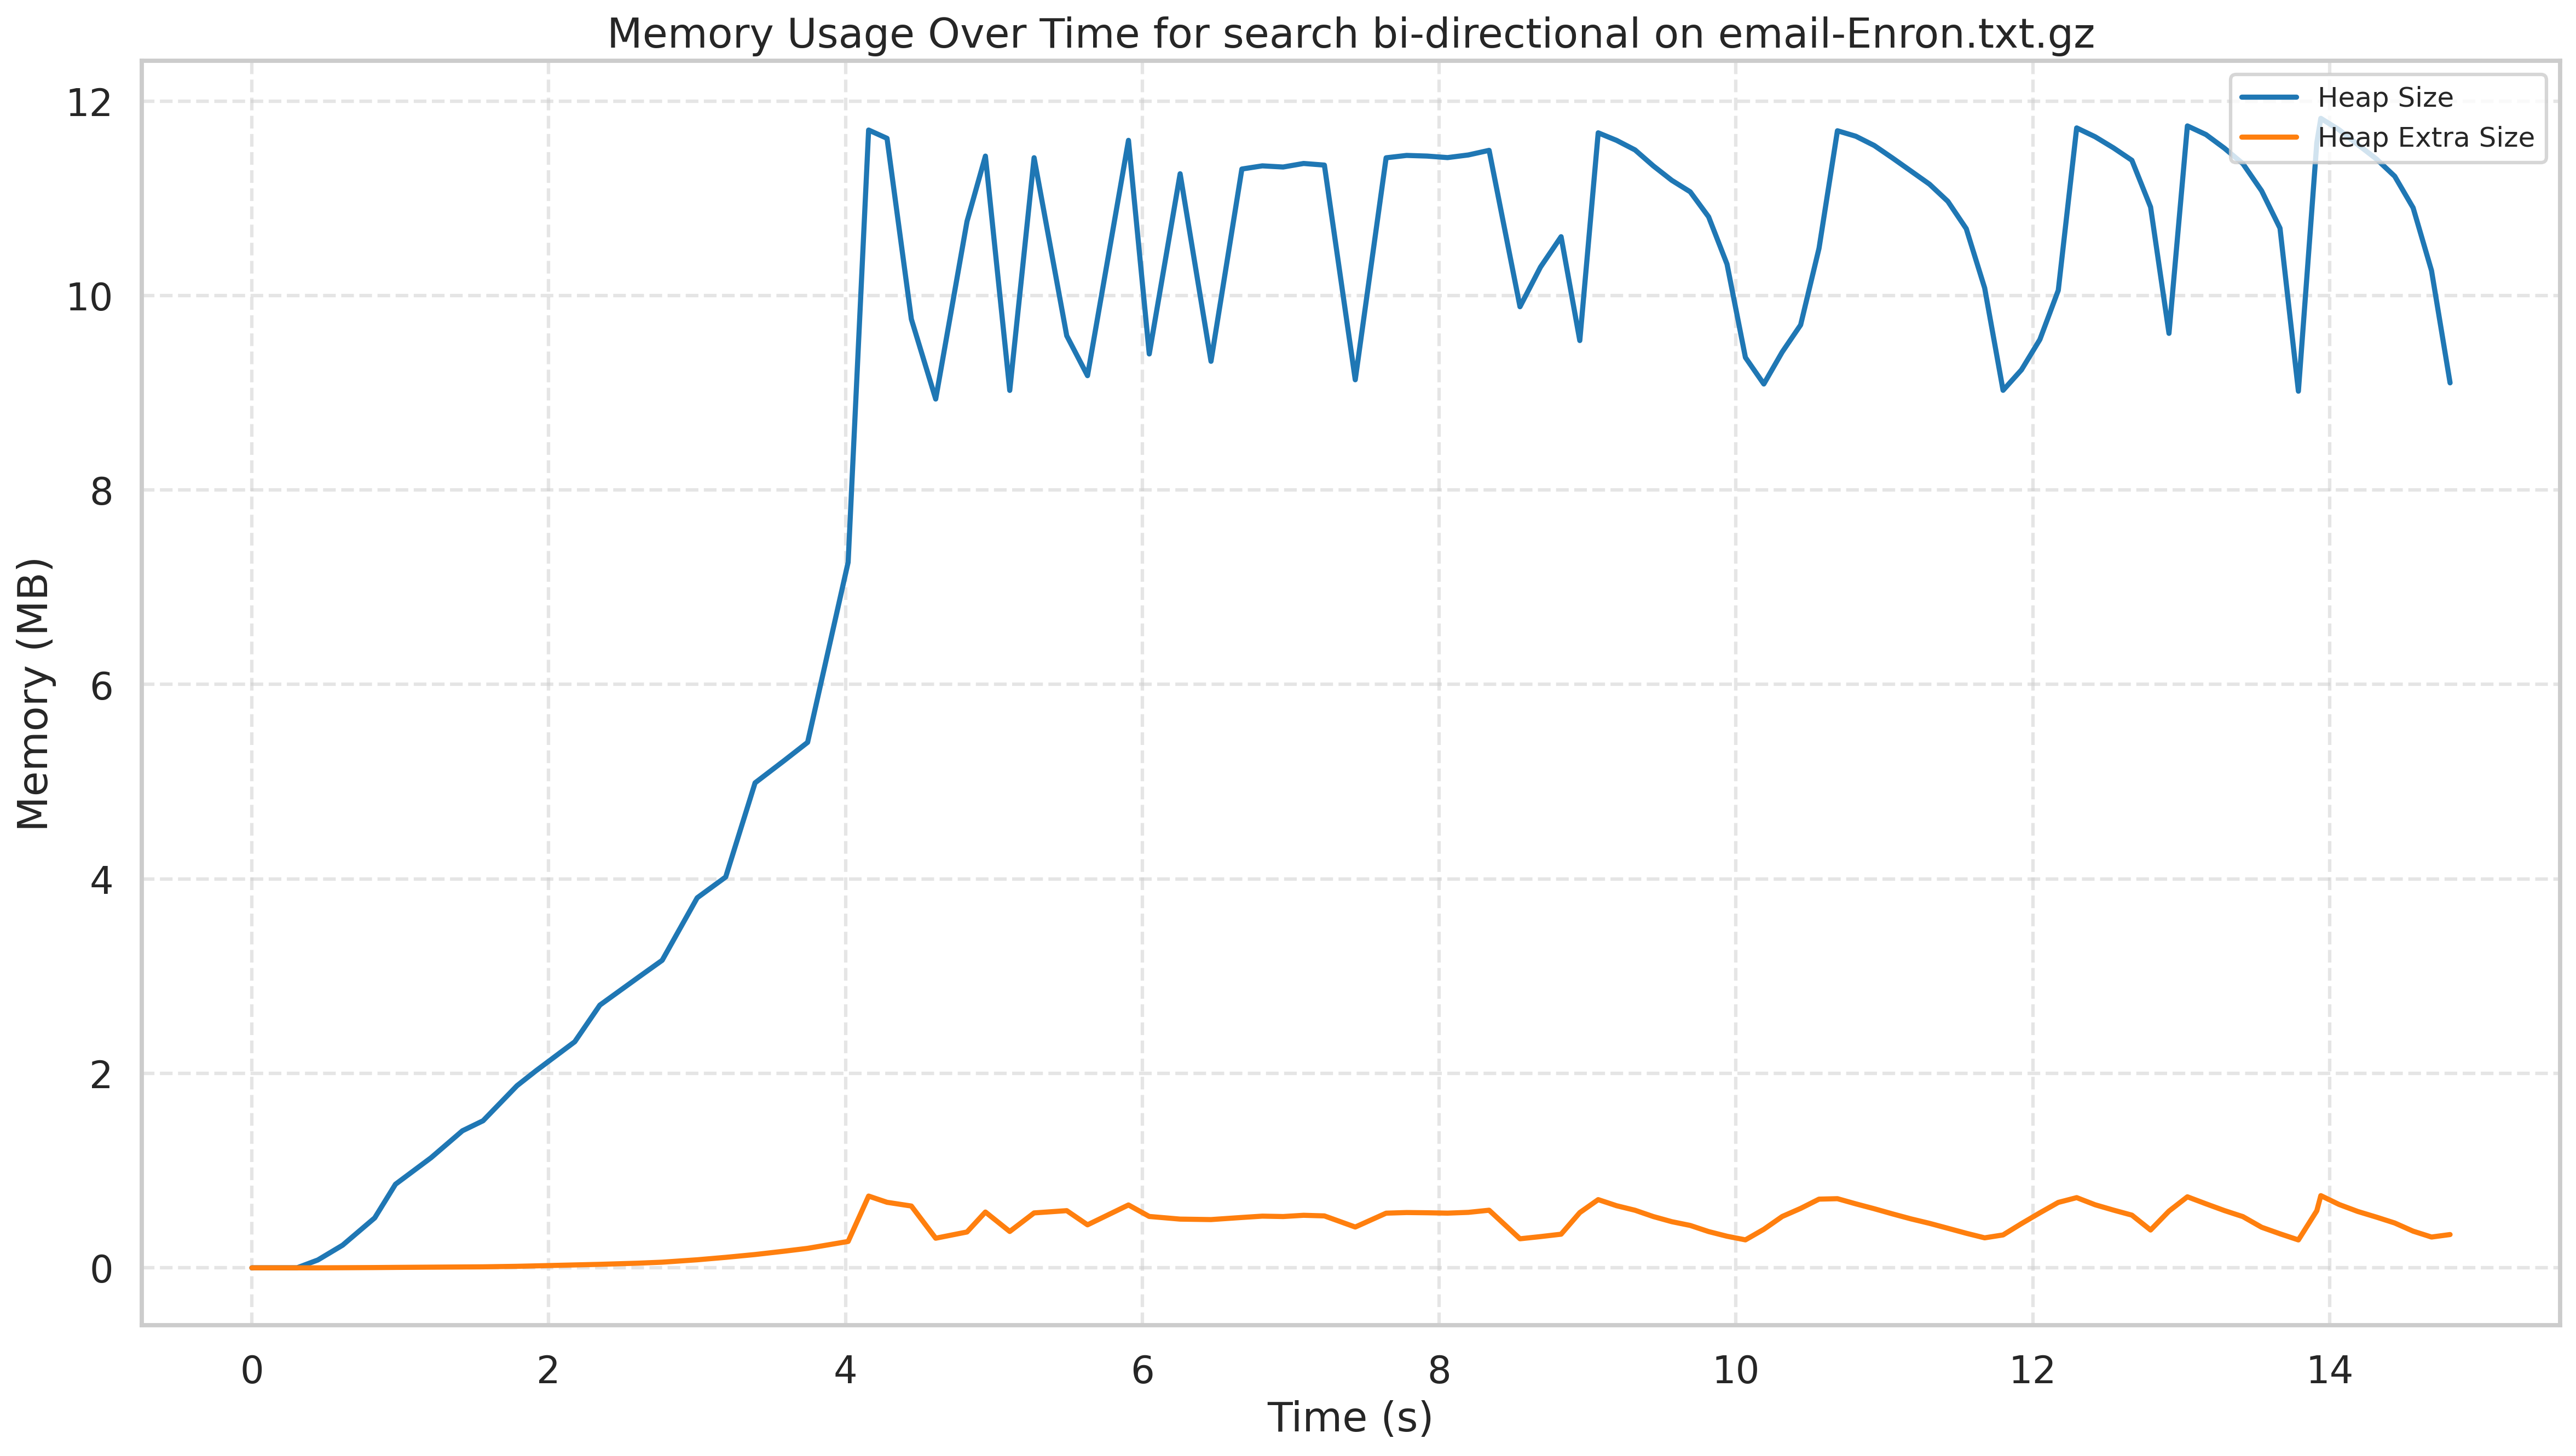
\includegraphics[width=\textwidth]{../plots/email-Enron_bi-directional.png}
\caption{Grafico: breadth-first su com-lj.ungraph}
\end{figure}
\subsubsection{Algoritmo di ricerca: breadth-first}
\begin{figure}[h]\centering
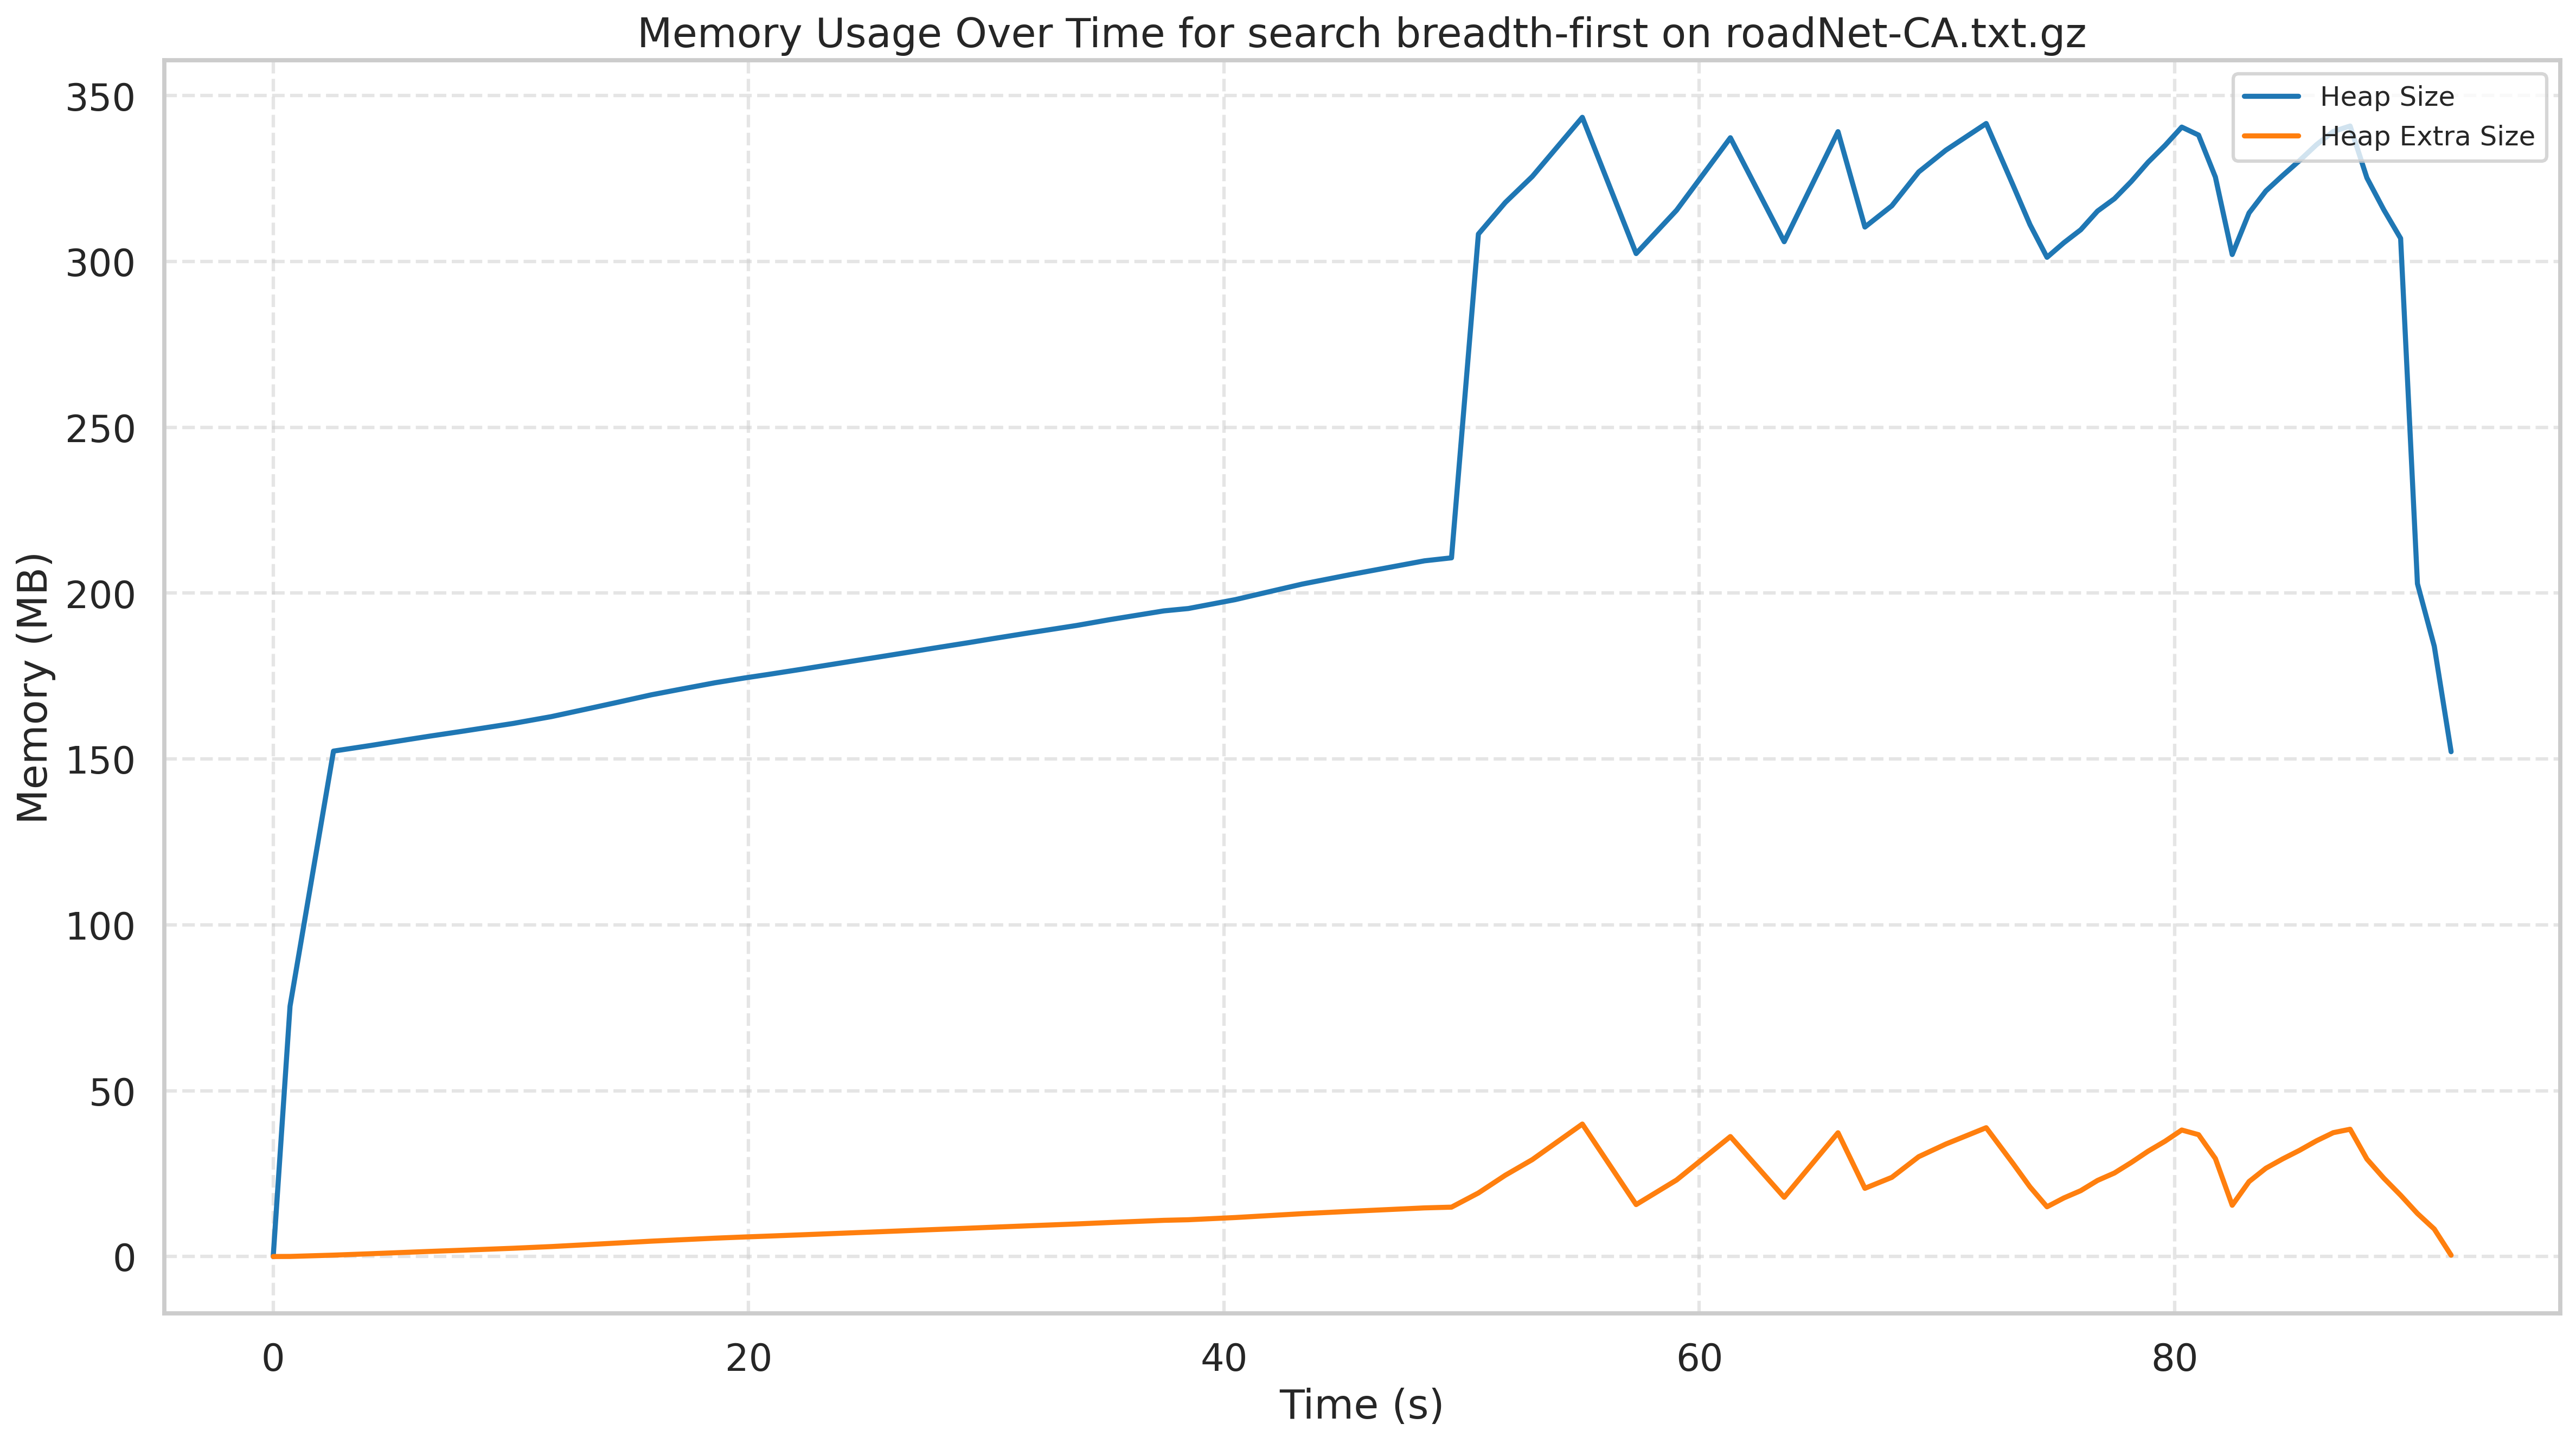
\includegraphics[width=\textwidth]{../plots/roadNet-CA_breadth-first.png}
\caption{Grafico: breadth-first su com-lj.ungraph}
\end{figure}
\subsubsection{Algoritmo di ricerca: uniform-cost}
\begin{figure}[h]\centering
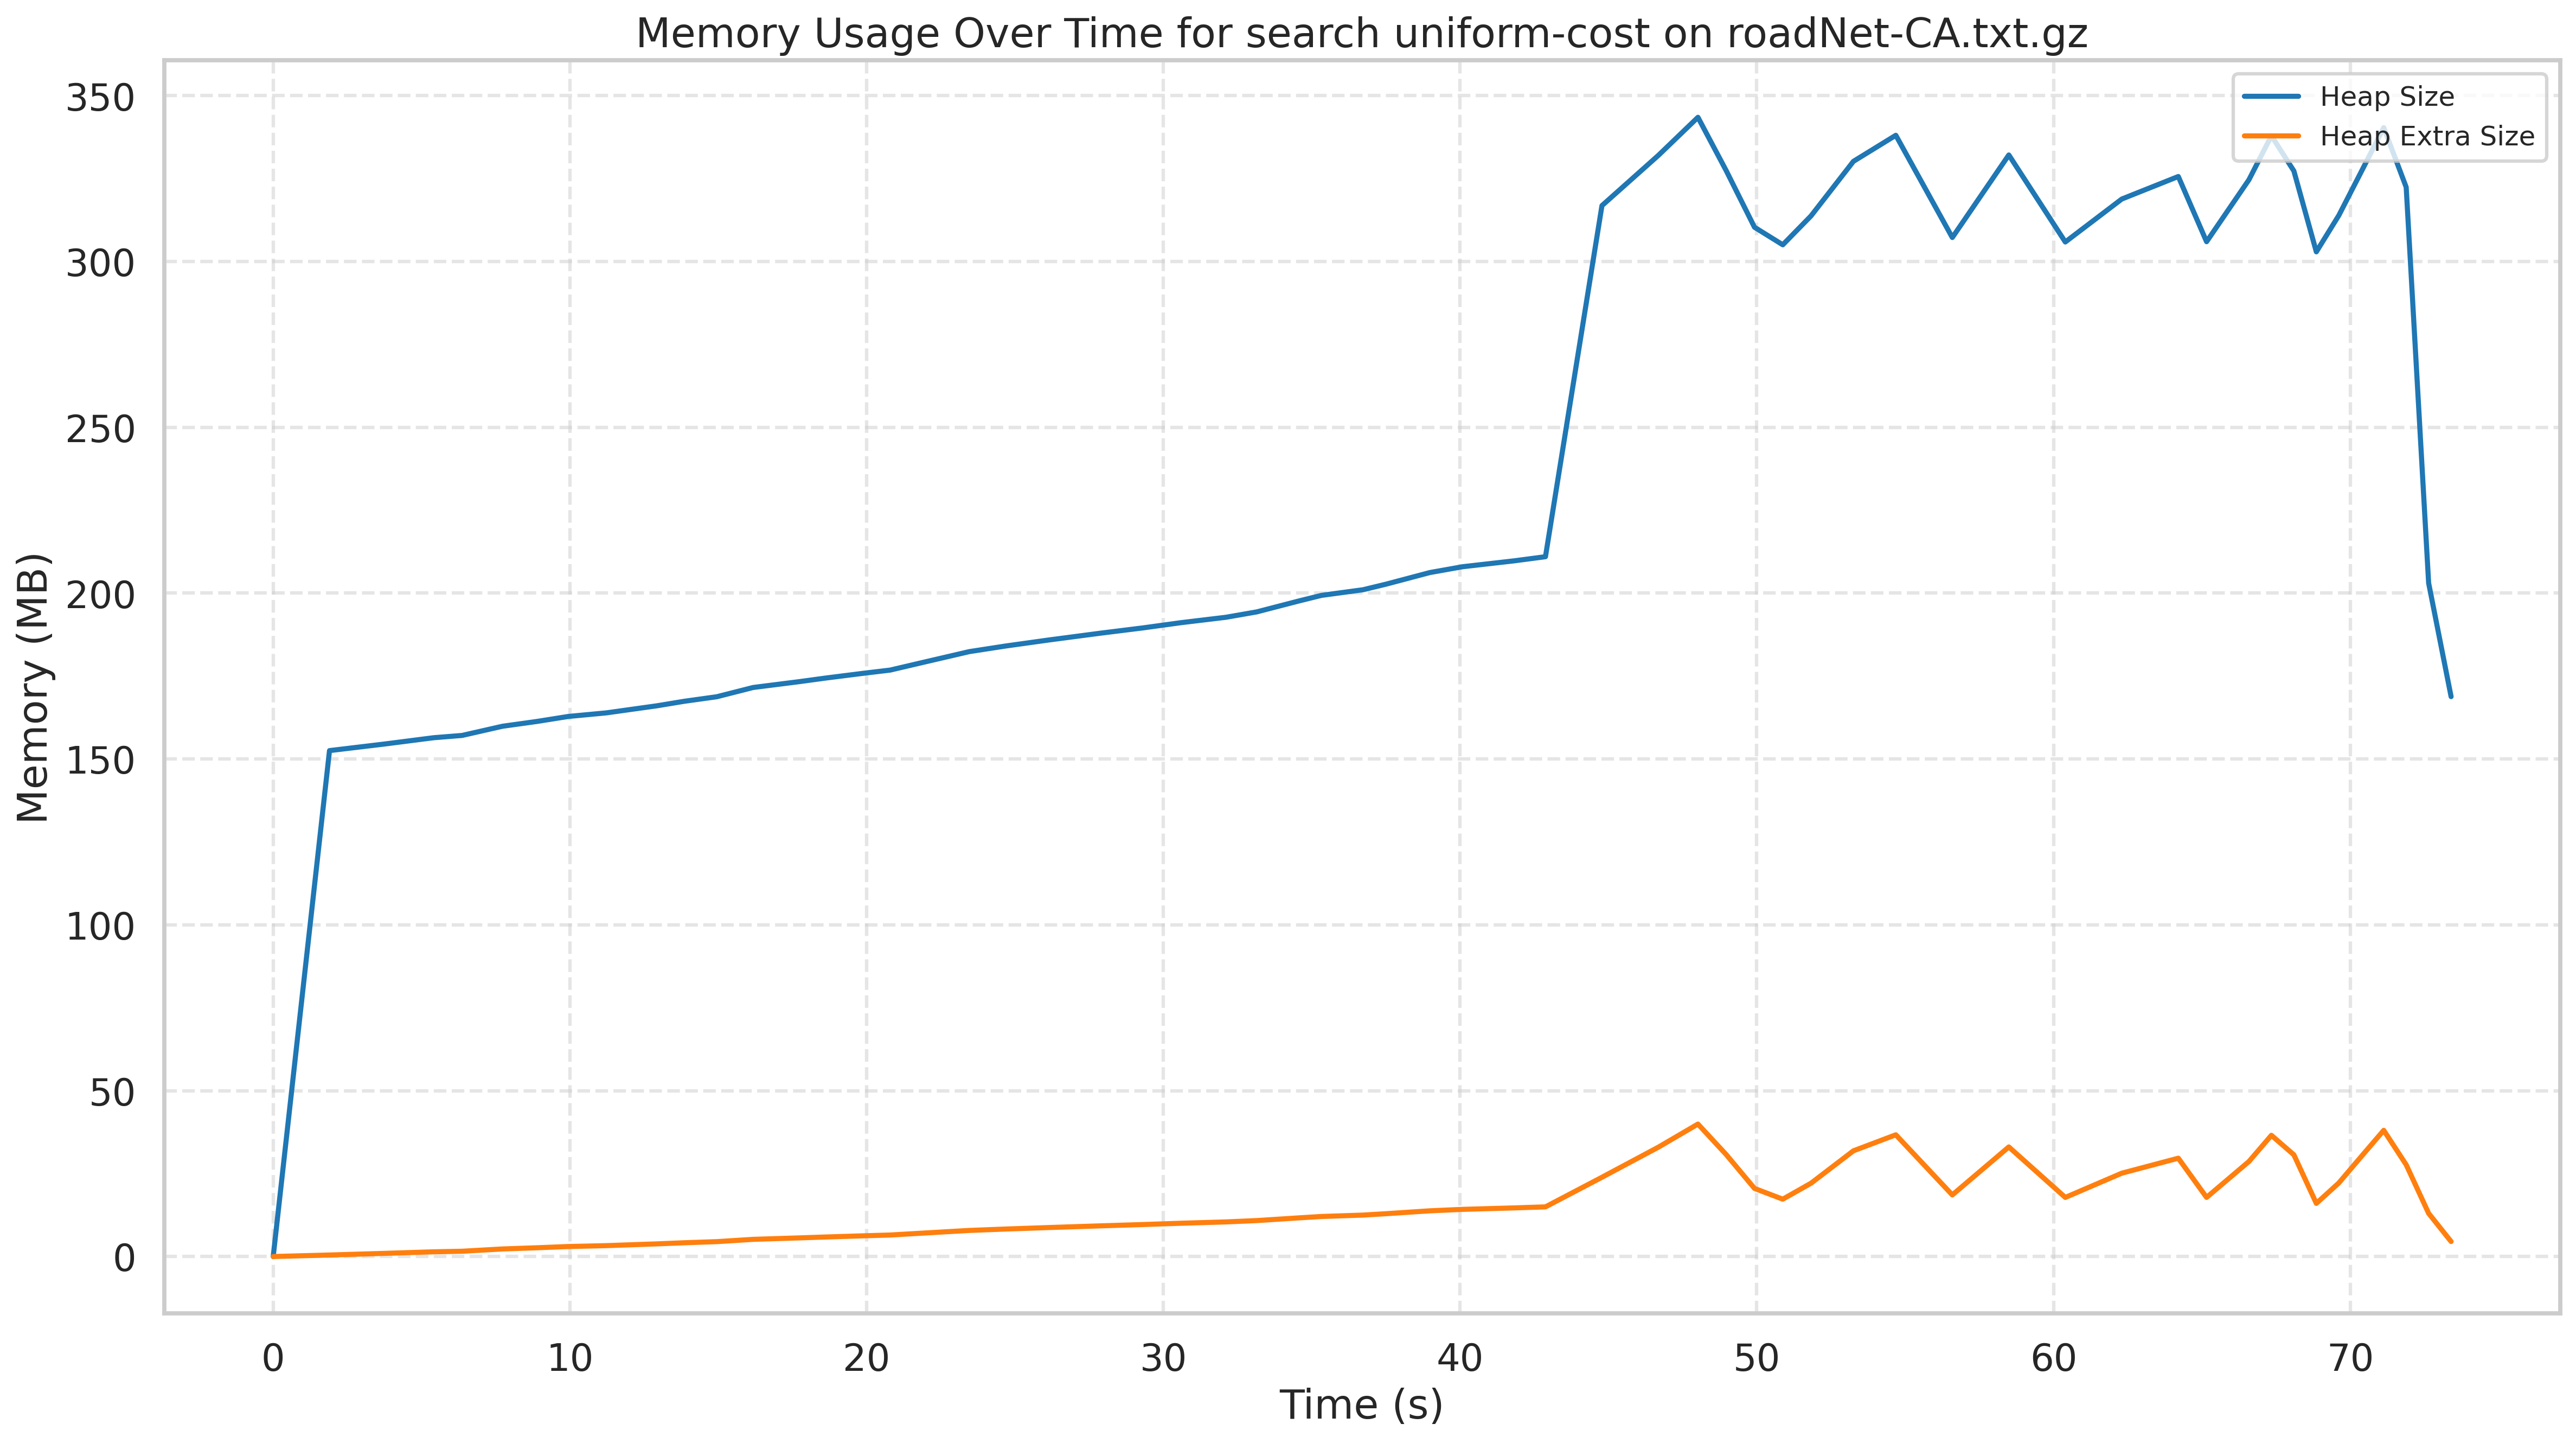
\includegraphics[width=\textwidth]{../plots/roadNet-CA_uniform-cost.png}
\caption{Grafico: breadth-first su com-lj.ungraph}
\end{figure}
\subsubsection{Algoritmo di ricerca: depth-limited}
\begin{figure}[h]\centering
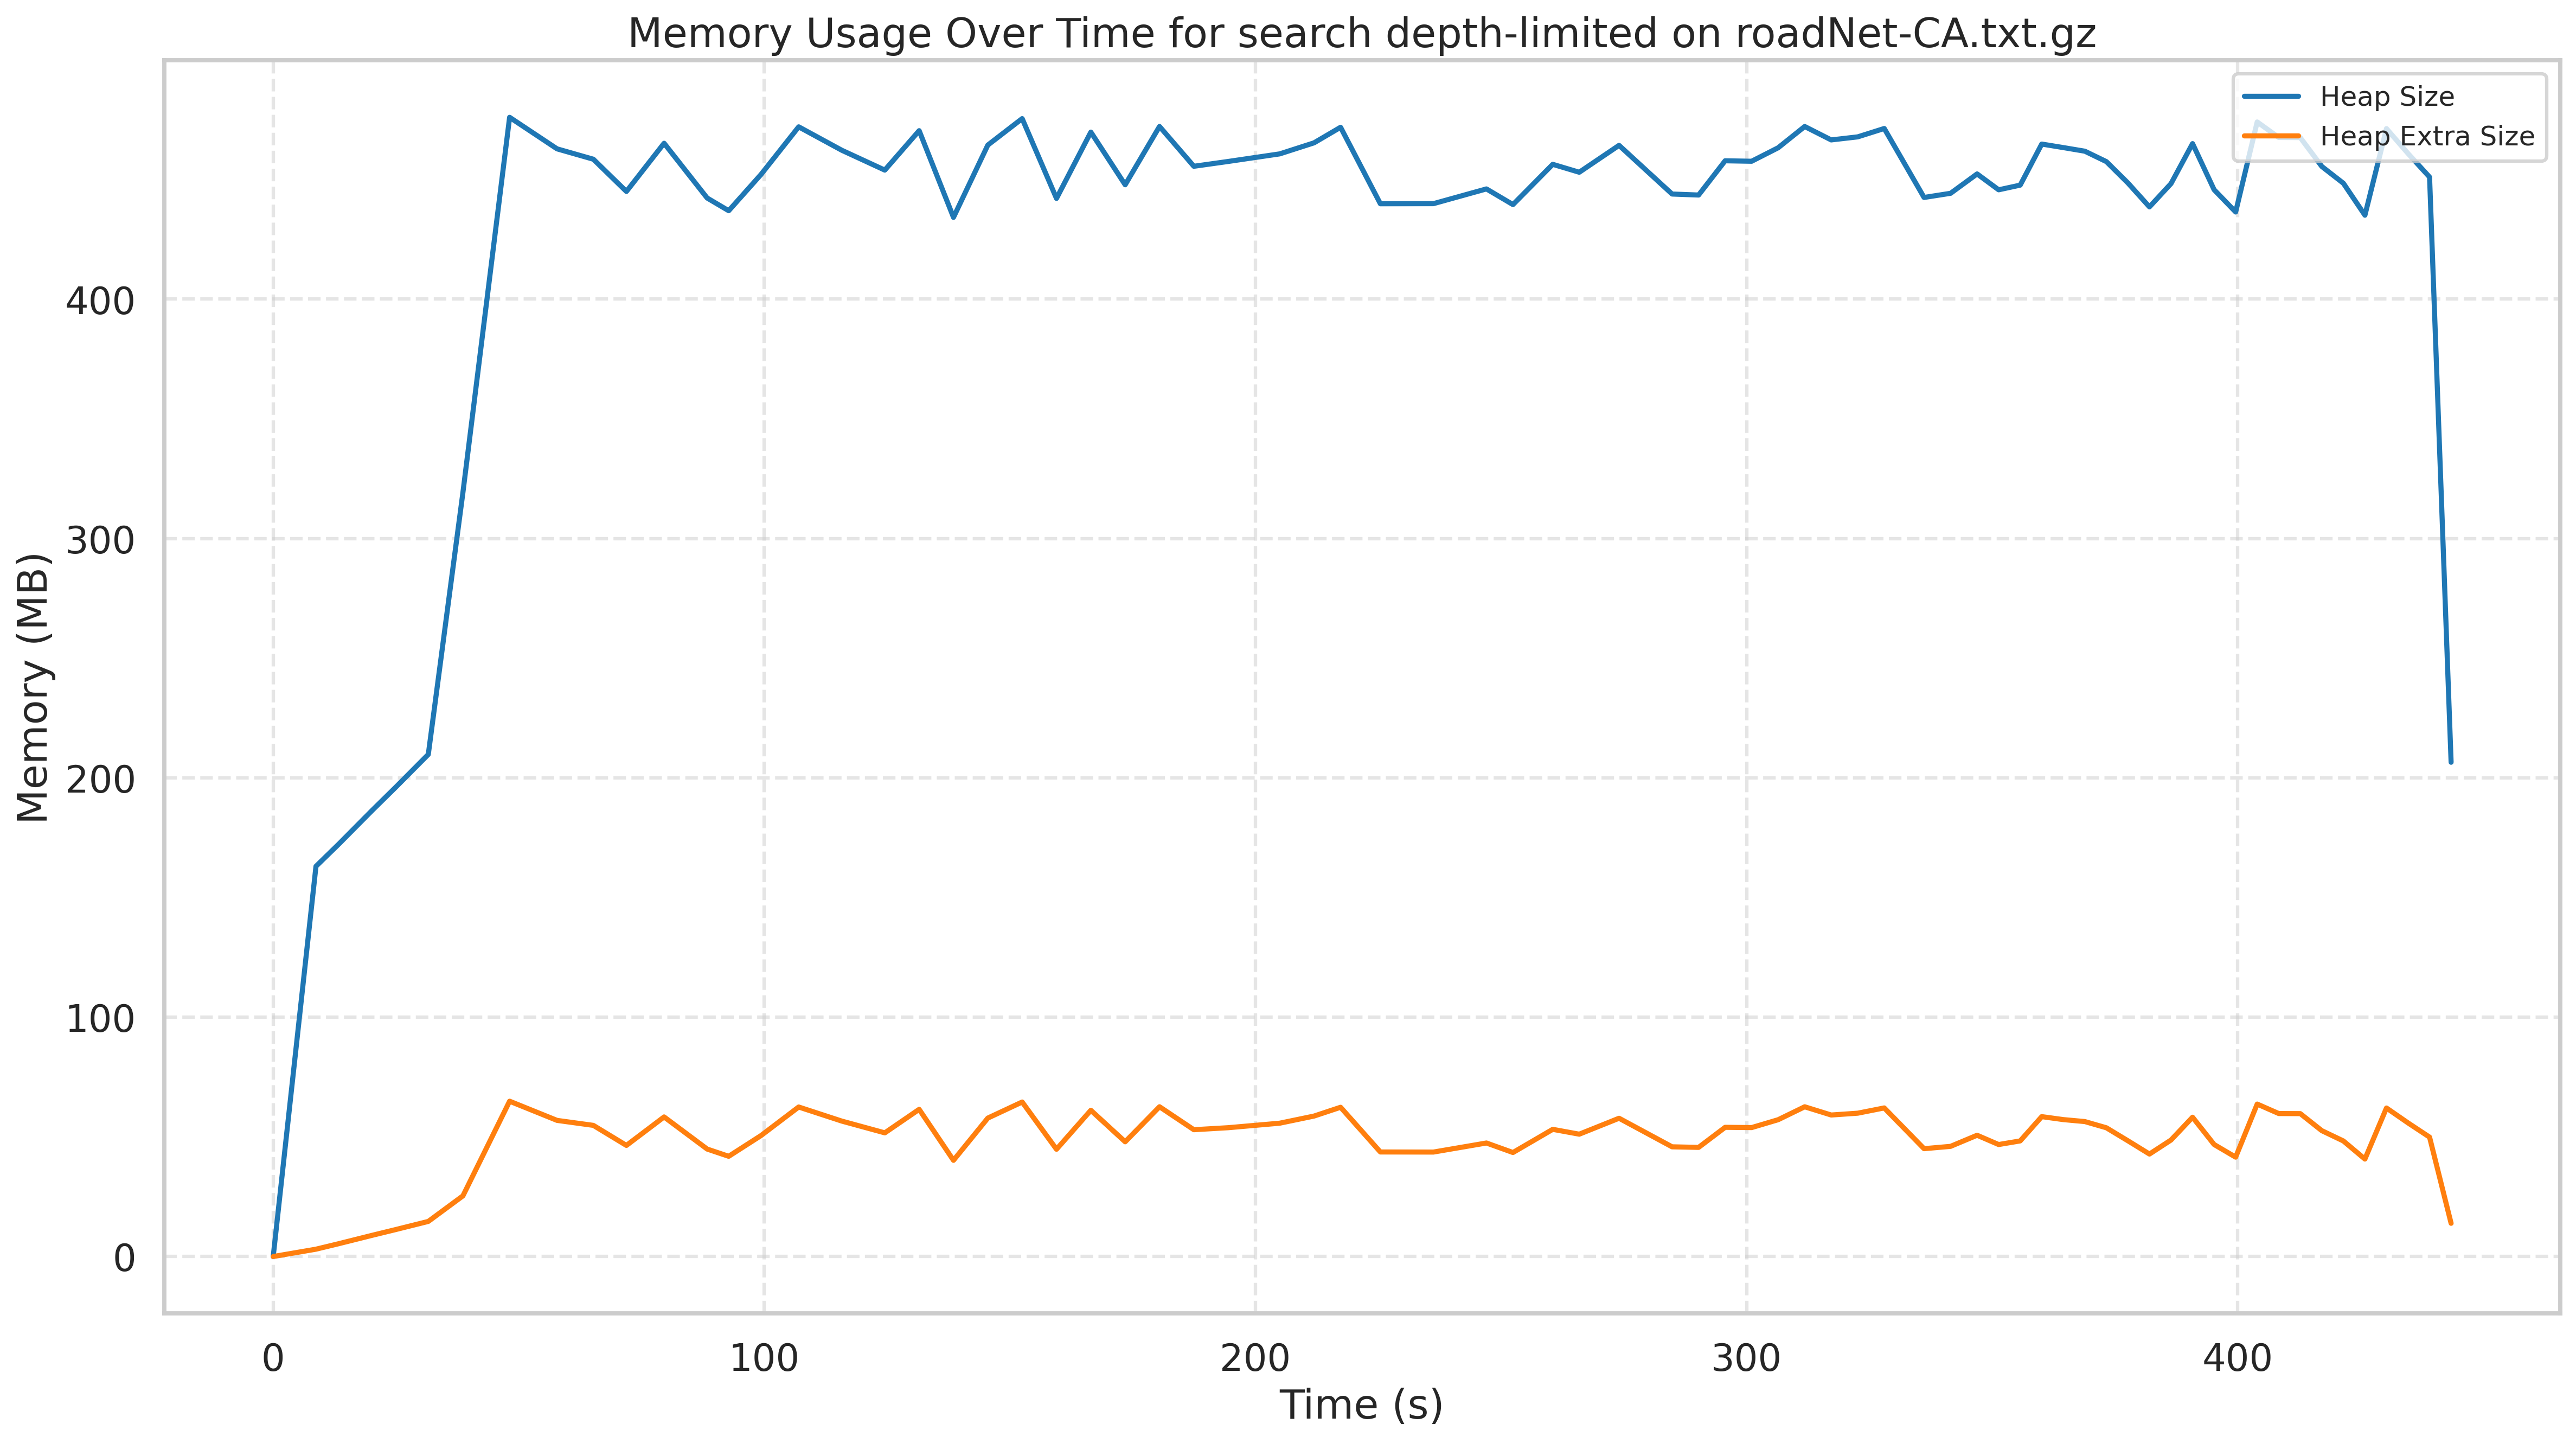
\includegraphics[width=\textwidth]{../plots/roadNet-CA_depth-limited.png}
\caption{Grafico: breadth-first su com-lj.ungraph}
\end{figure}
\subsubsection{Algoritmo di ricerca: iterative-deepening}
\begin{figure}[h]\centering
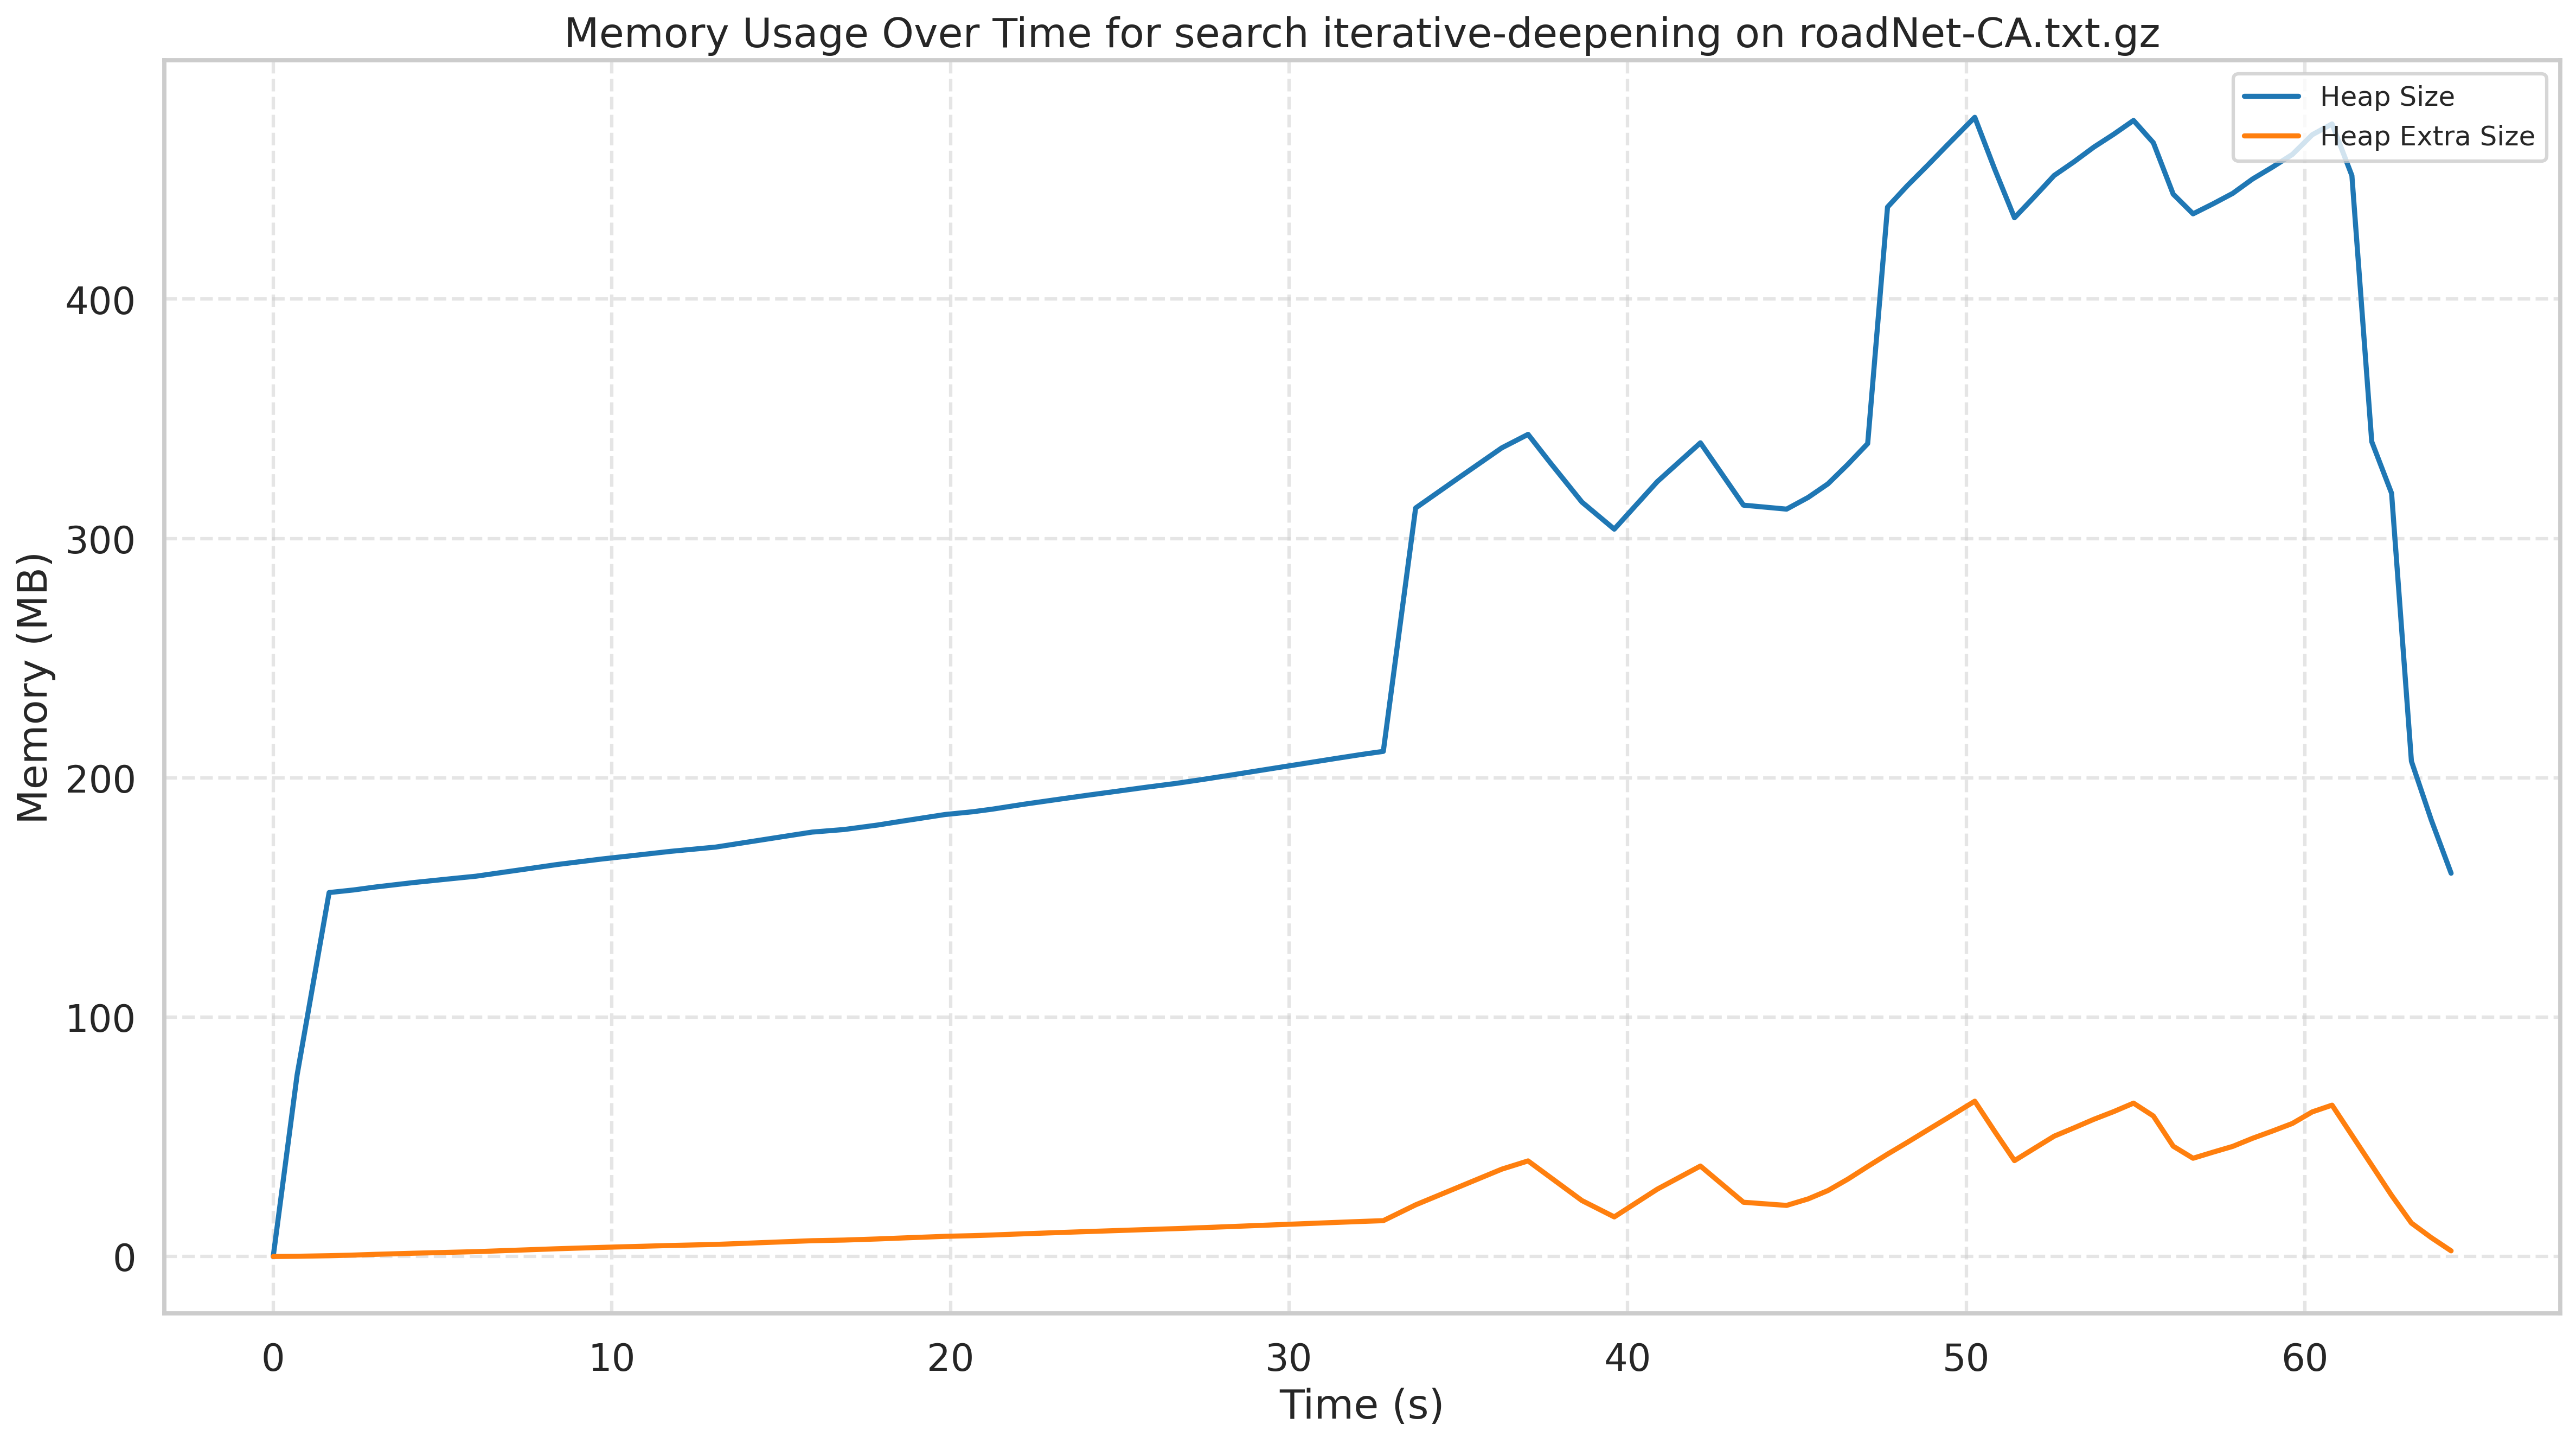
\includegraphics[width=\textwidth]{../plots/roadNet-CA_iterative-deepening.png}
\caption{Grafico: breadth-first su com-lj.ungraph}
\end{figure}
\subsubsection{Algoritmo di ricerca: bi-directional}
\begin{figure}[h]\centering
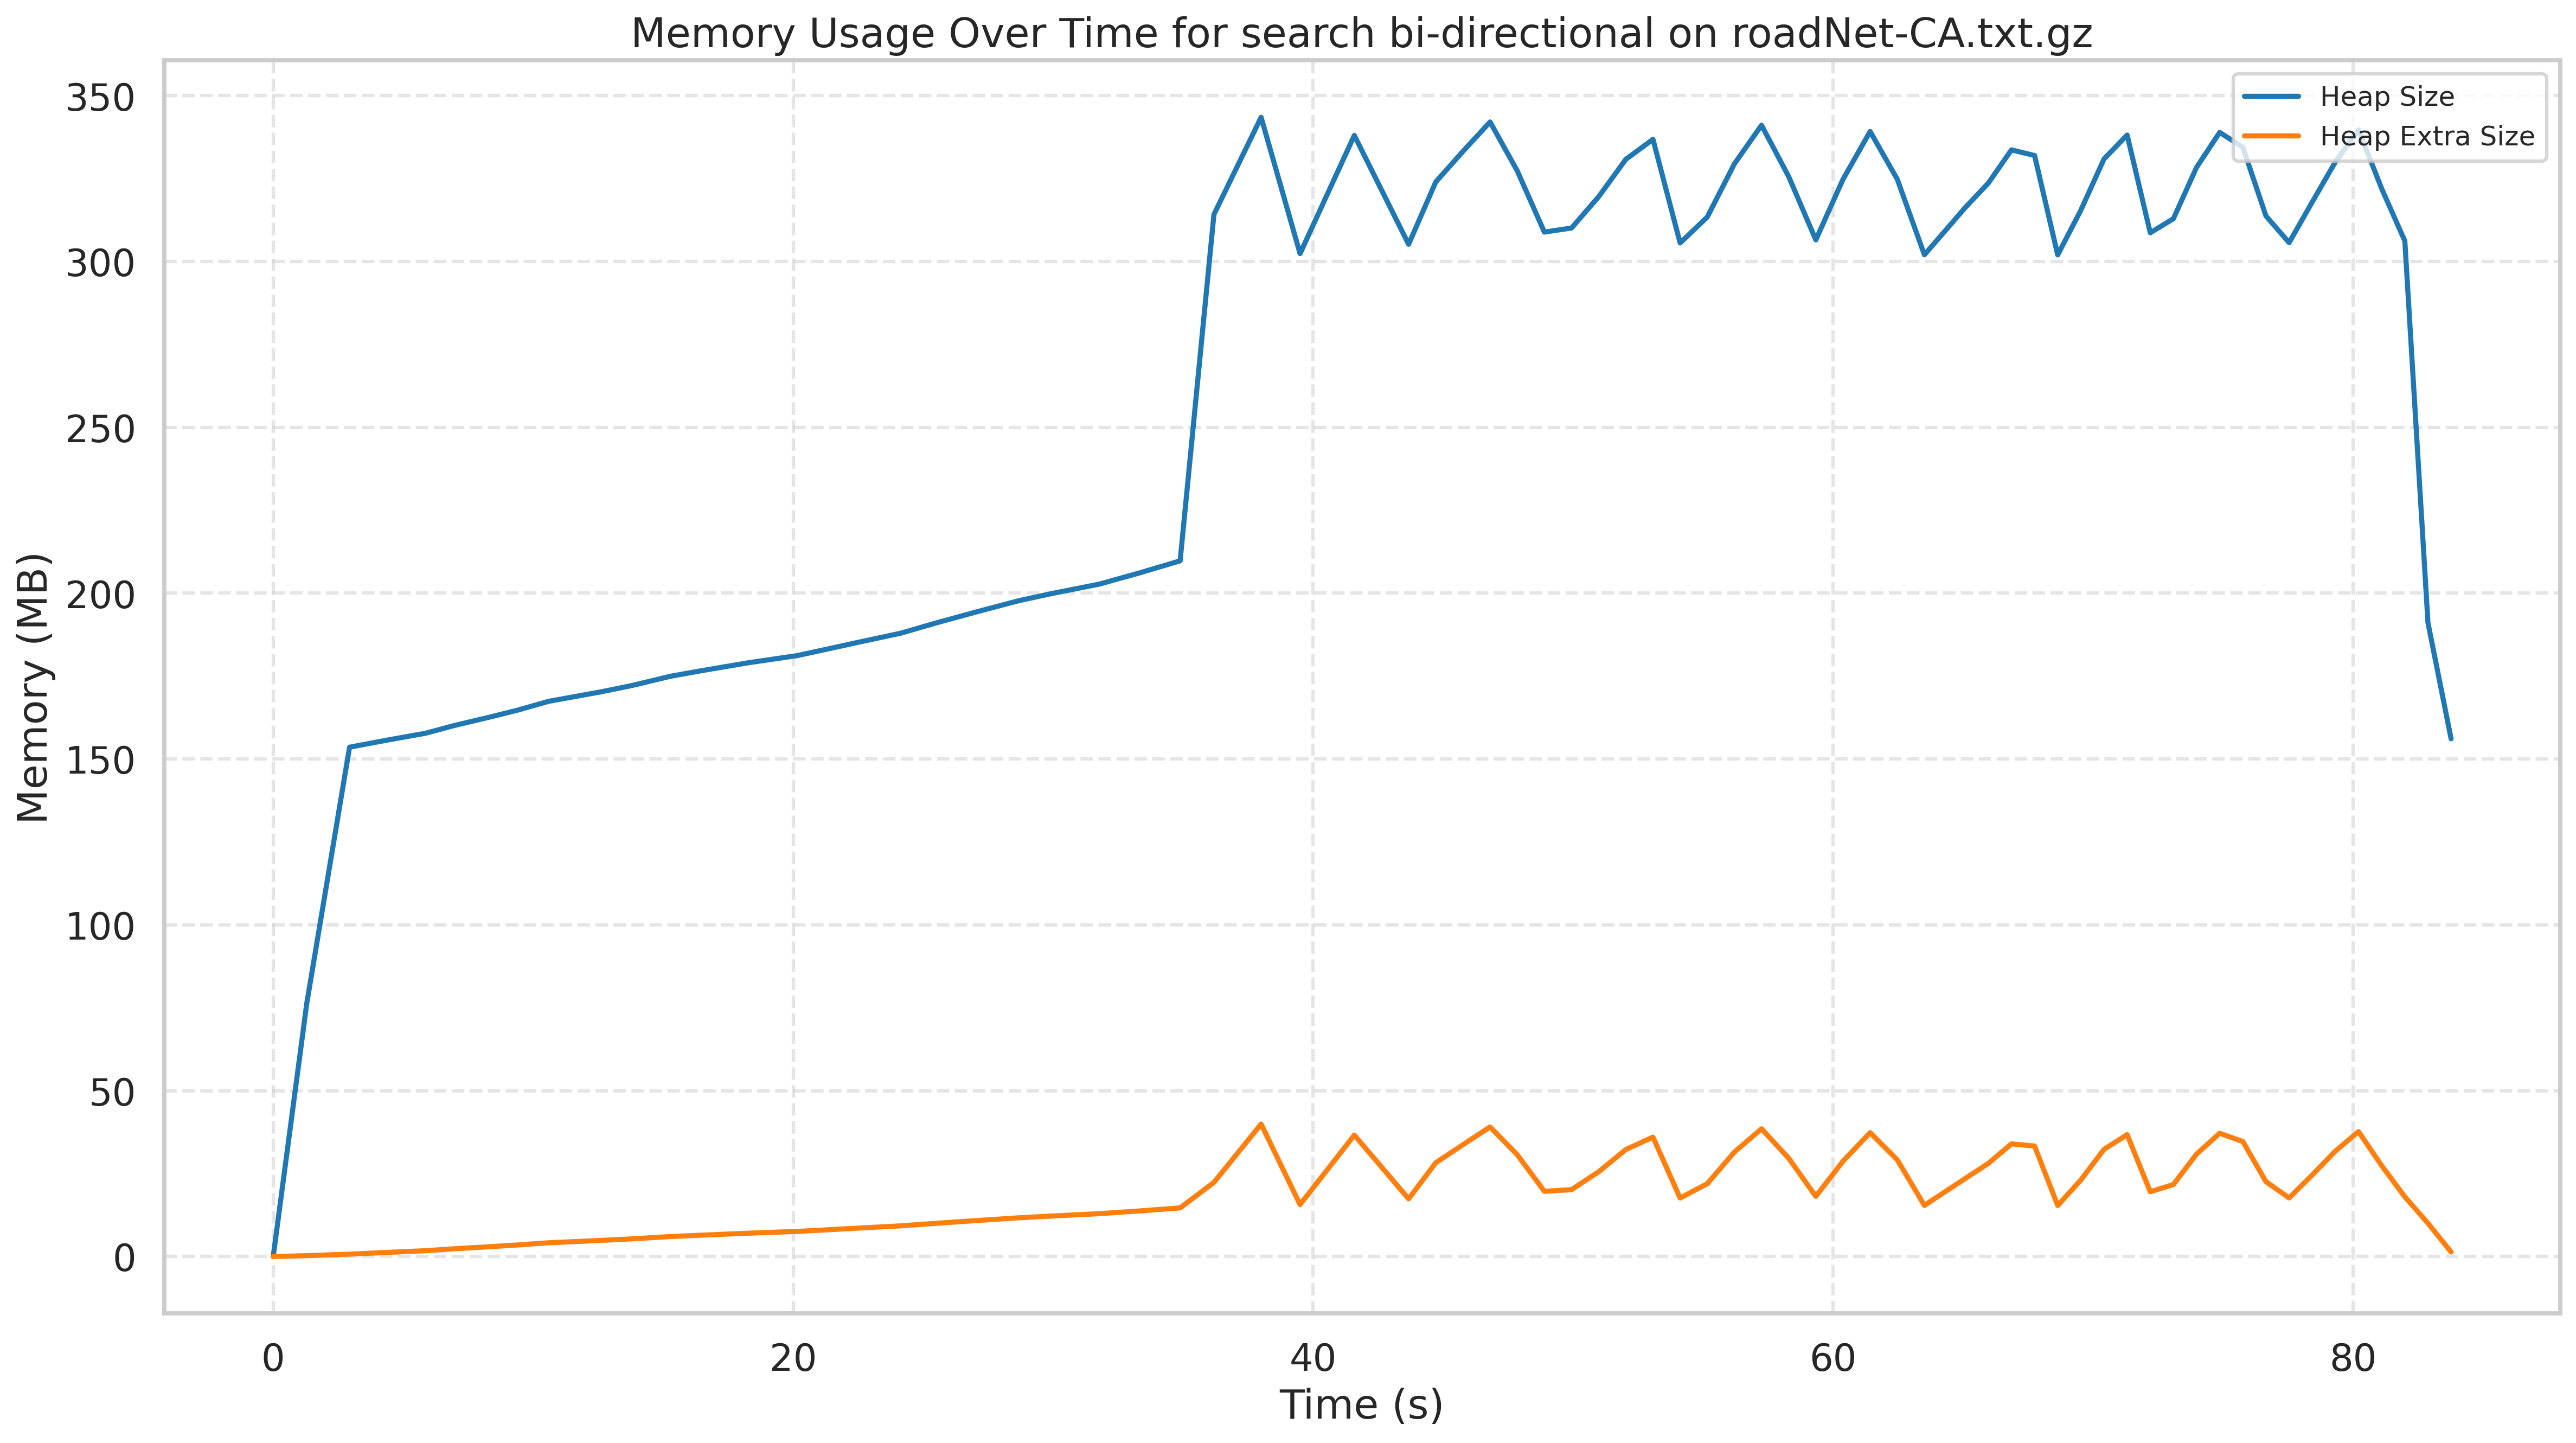
\includegraphics[width=\textwidth]{../plots/roadNet-CA_bi-directional.png}
\caption{Grafico: breadth-first su com-lj.ungraph}
\end{figure}
\subsubsection{Algoritmo di ricerca: breadth-first}
\begin{figure}[h]\centering
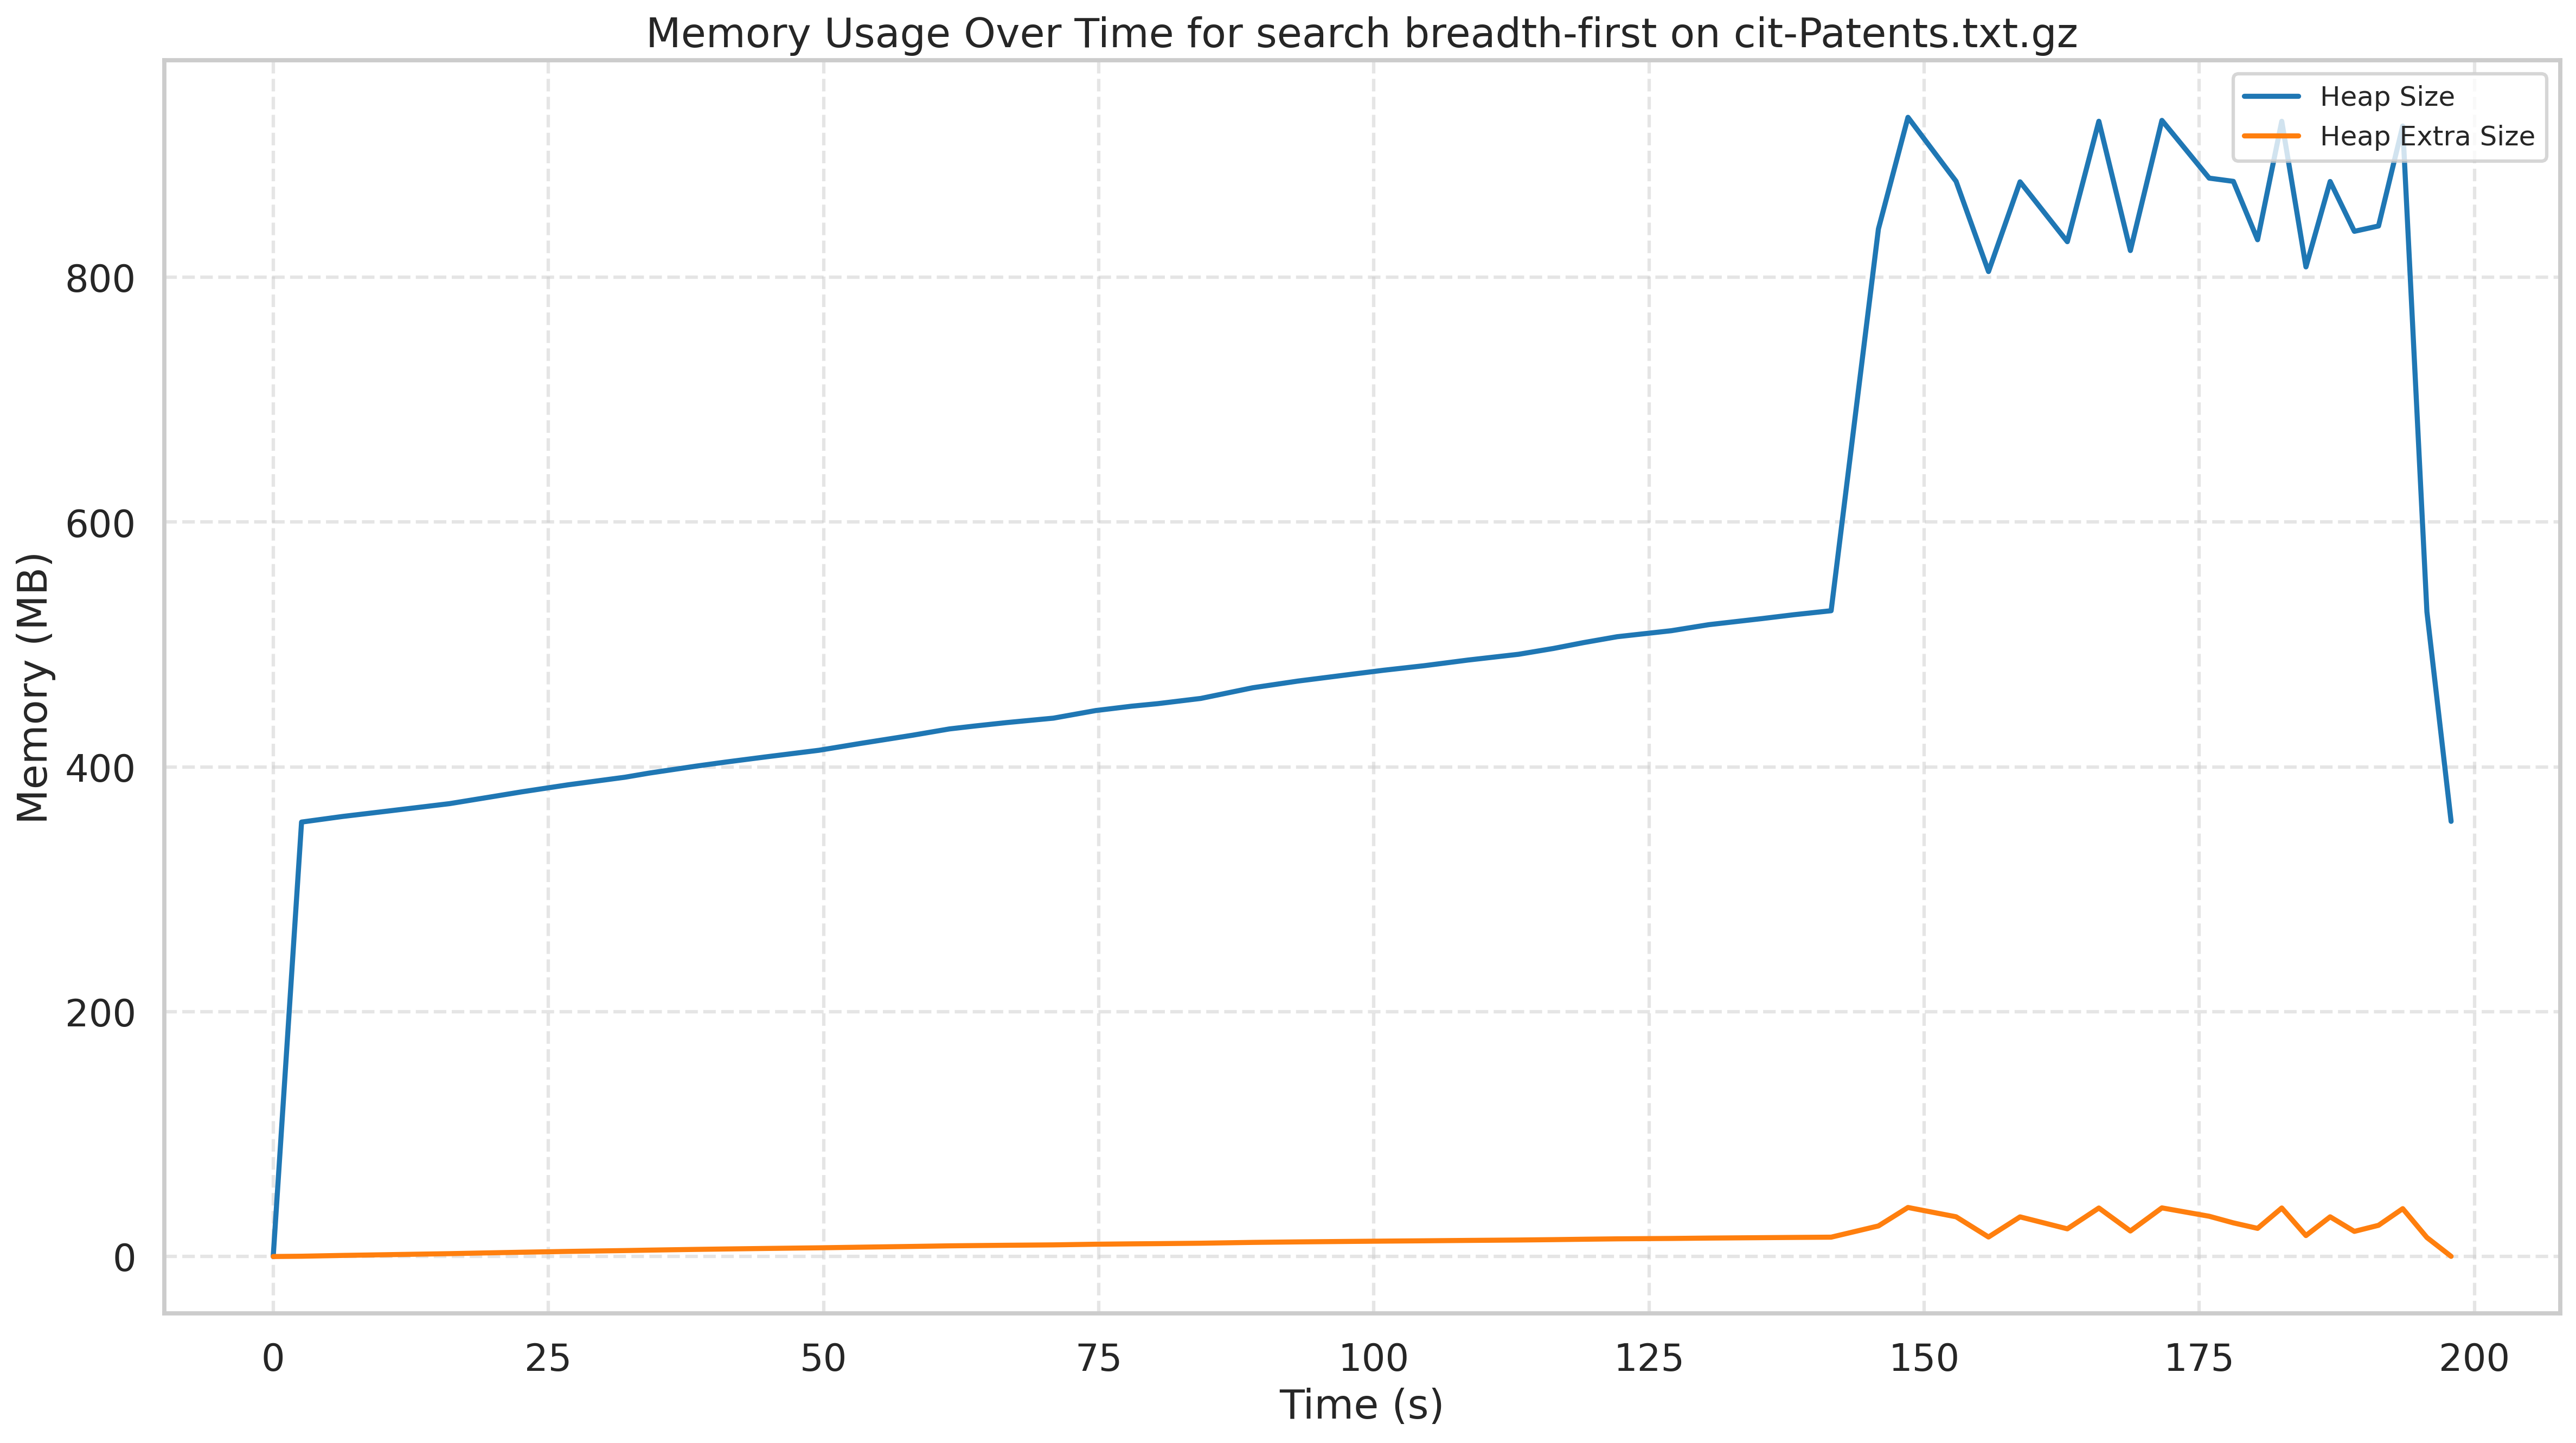
\includegraphics[width=\textwidth]{../plots/cit-Patents_breadth-first.png}
\caption{Grafico: breadth-first su com-lj.ungraph}
\end{figure}
\subsubsection{Algoritmo di ricerca: uniform-cost}
\begin{figure}[h]\centering
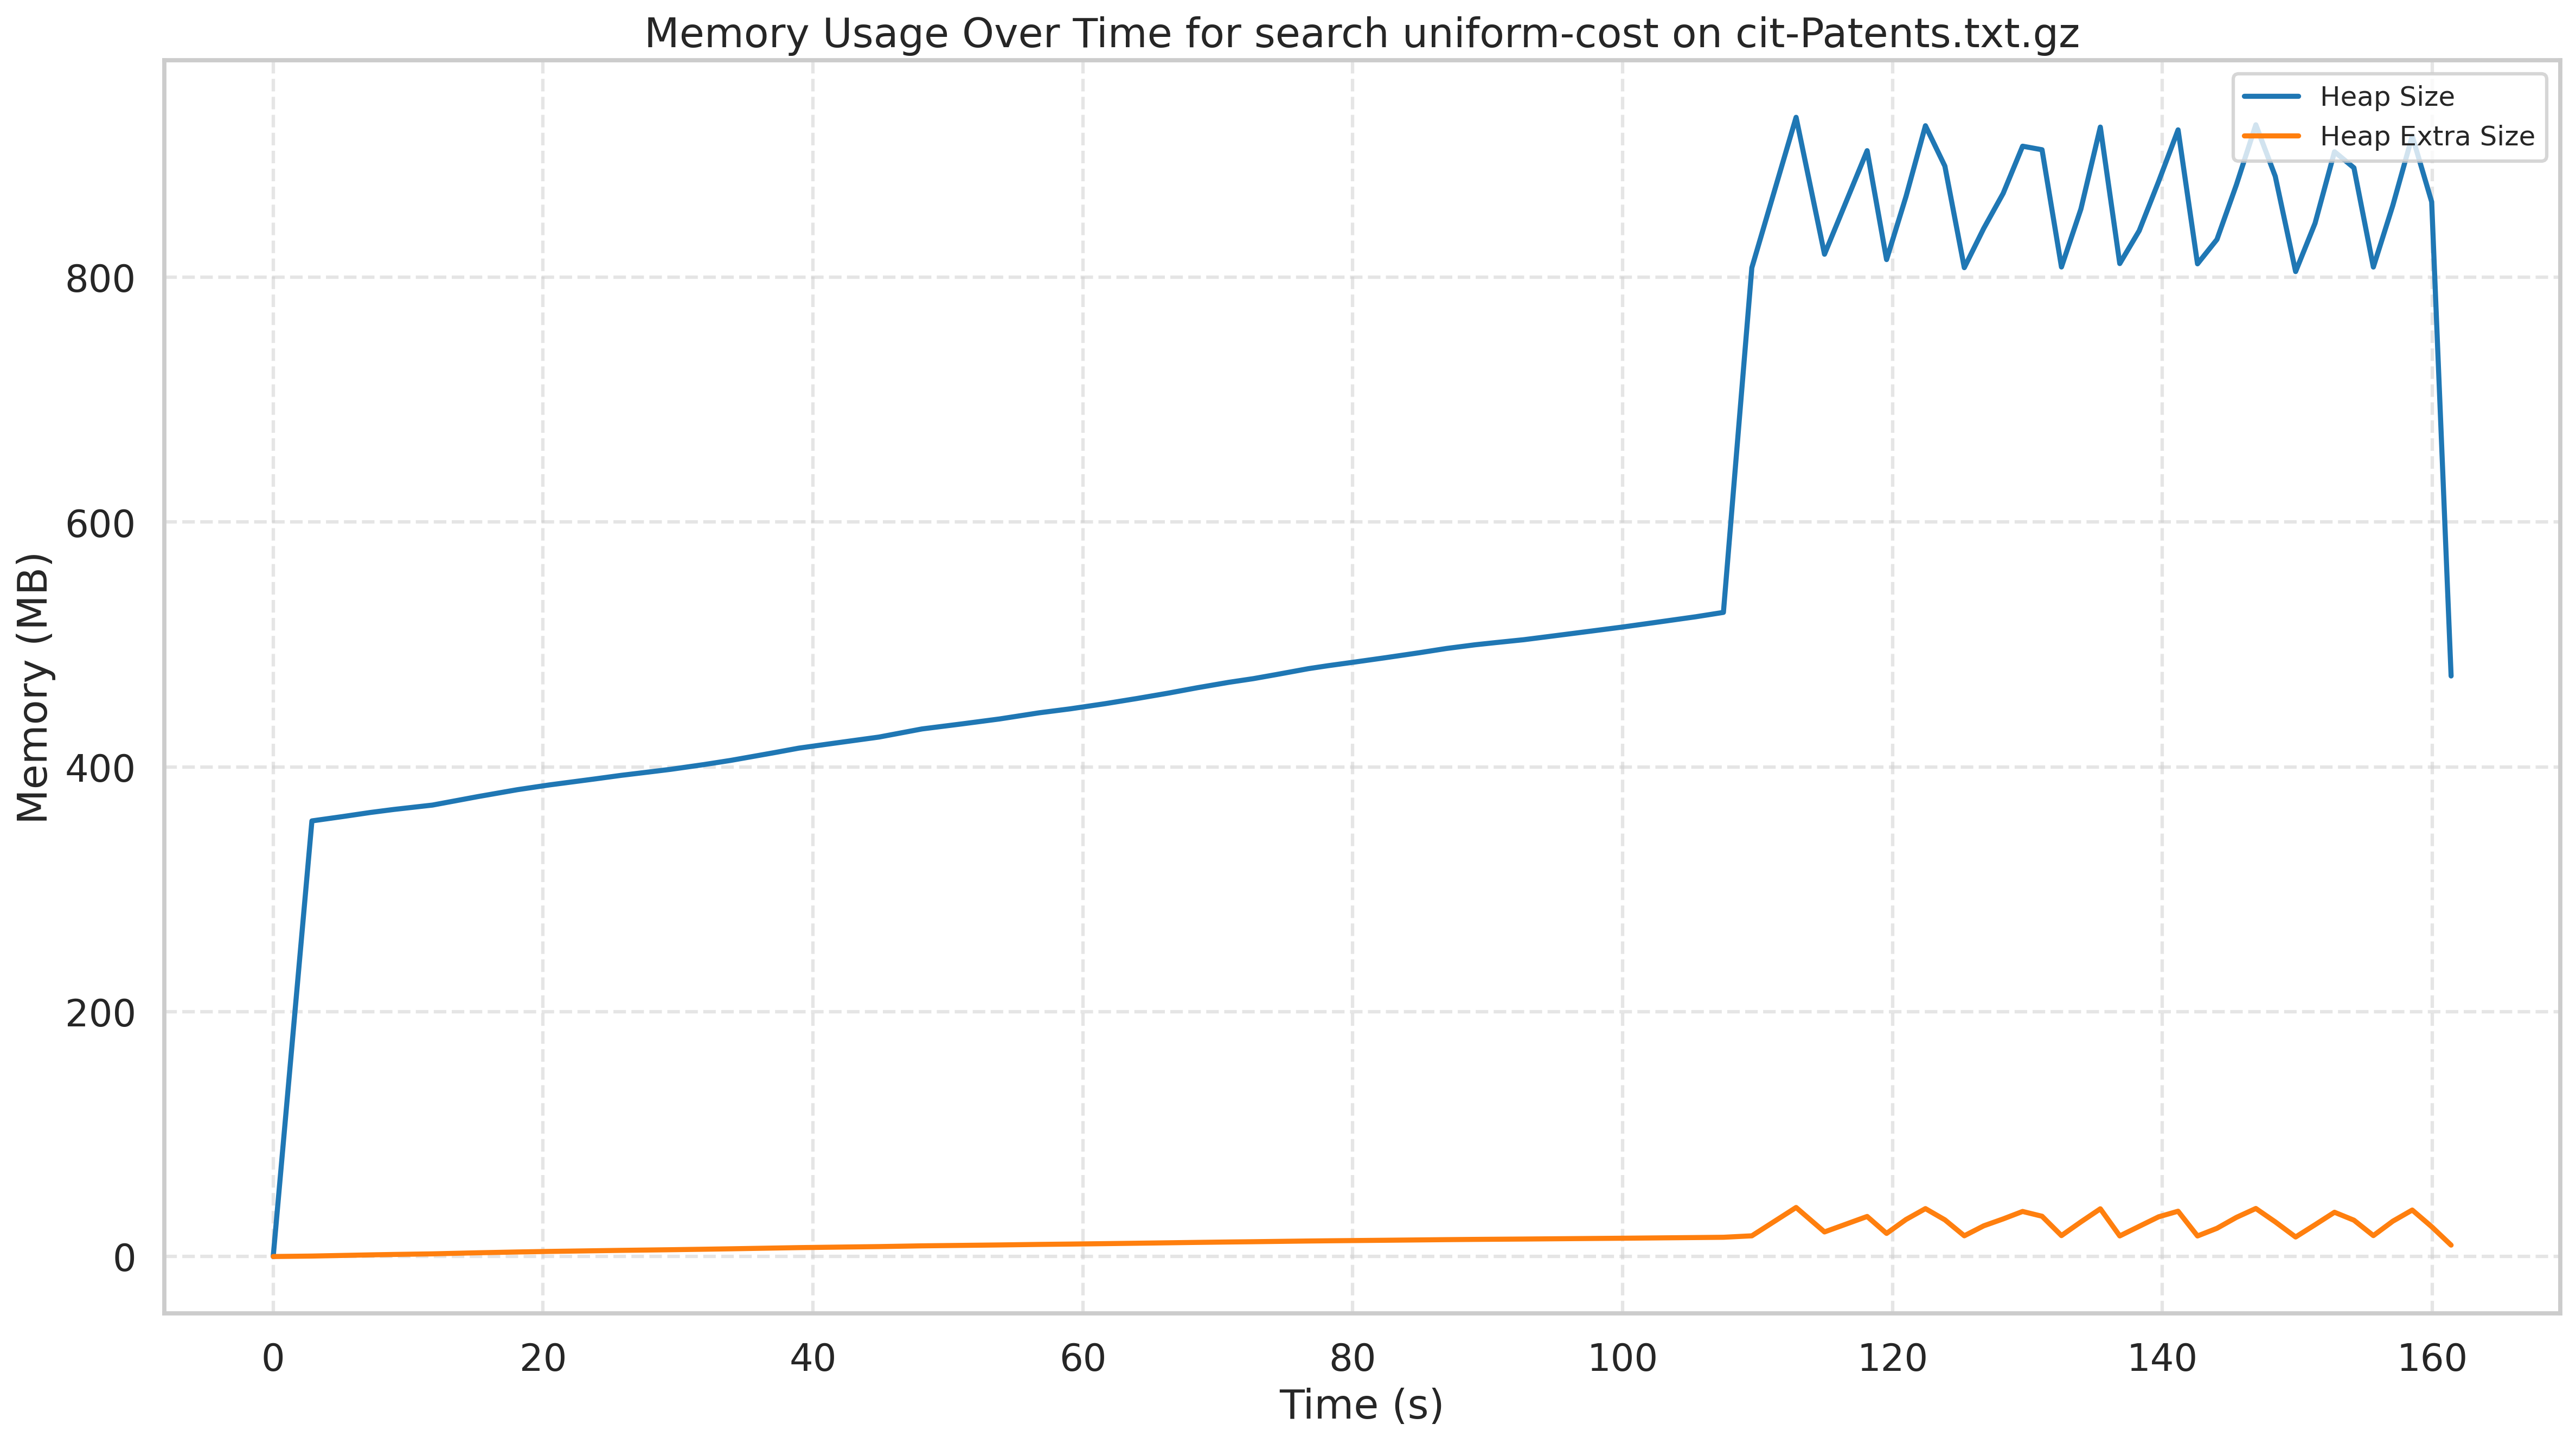
\includegraphics[width=\textwidth]{../plots/cit-Patents_uniform-cost.png}
\caption{Grafico: breadth-first su com-lj.ungraph}
\end{figure}
\subsubsection{Algoritmo di ricerca: depth-limited}
\begin{figure}[h]\centering
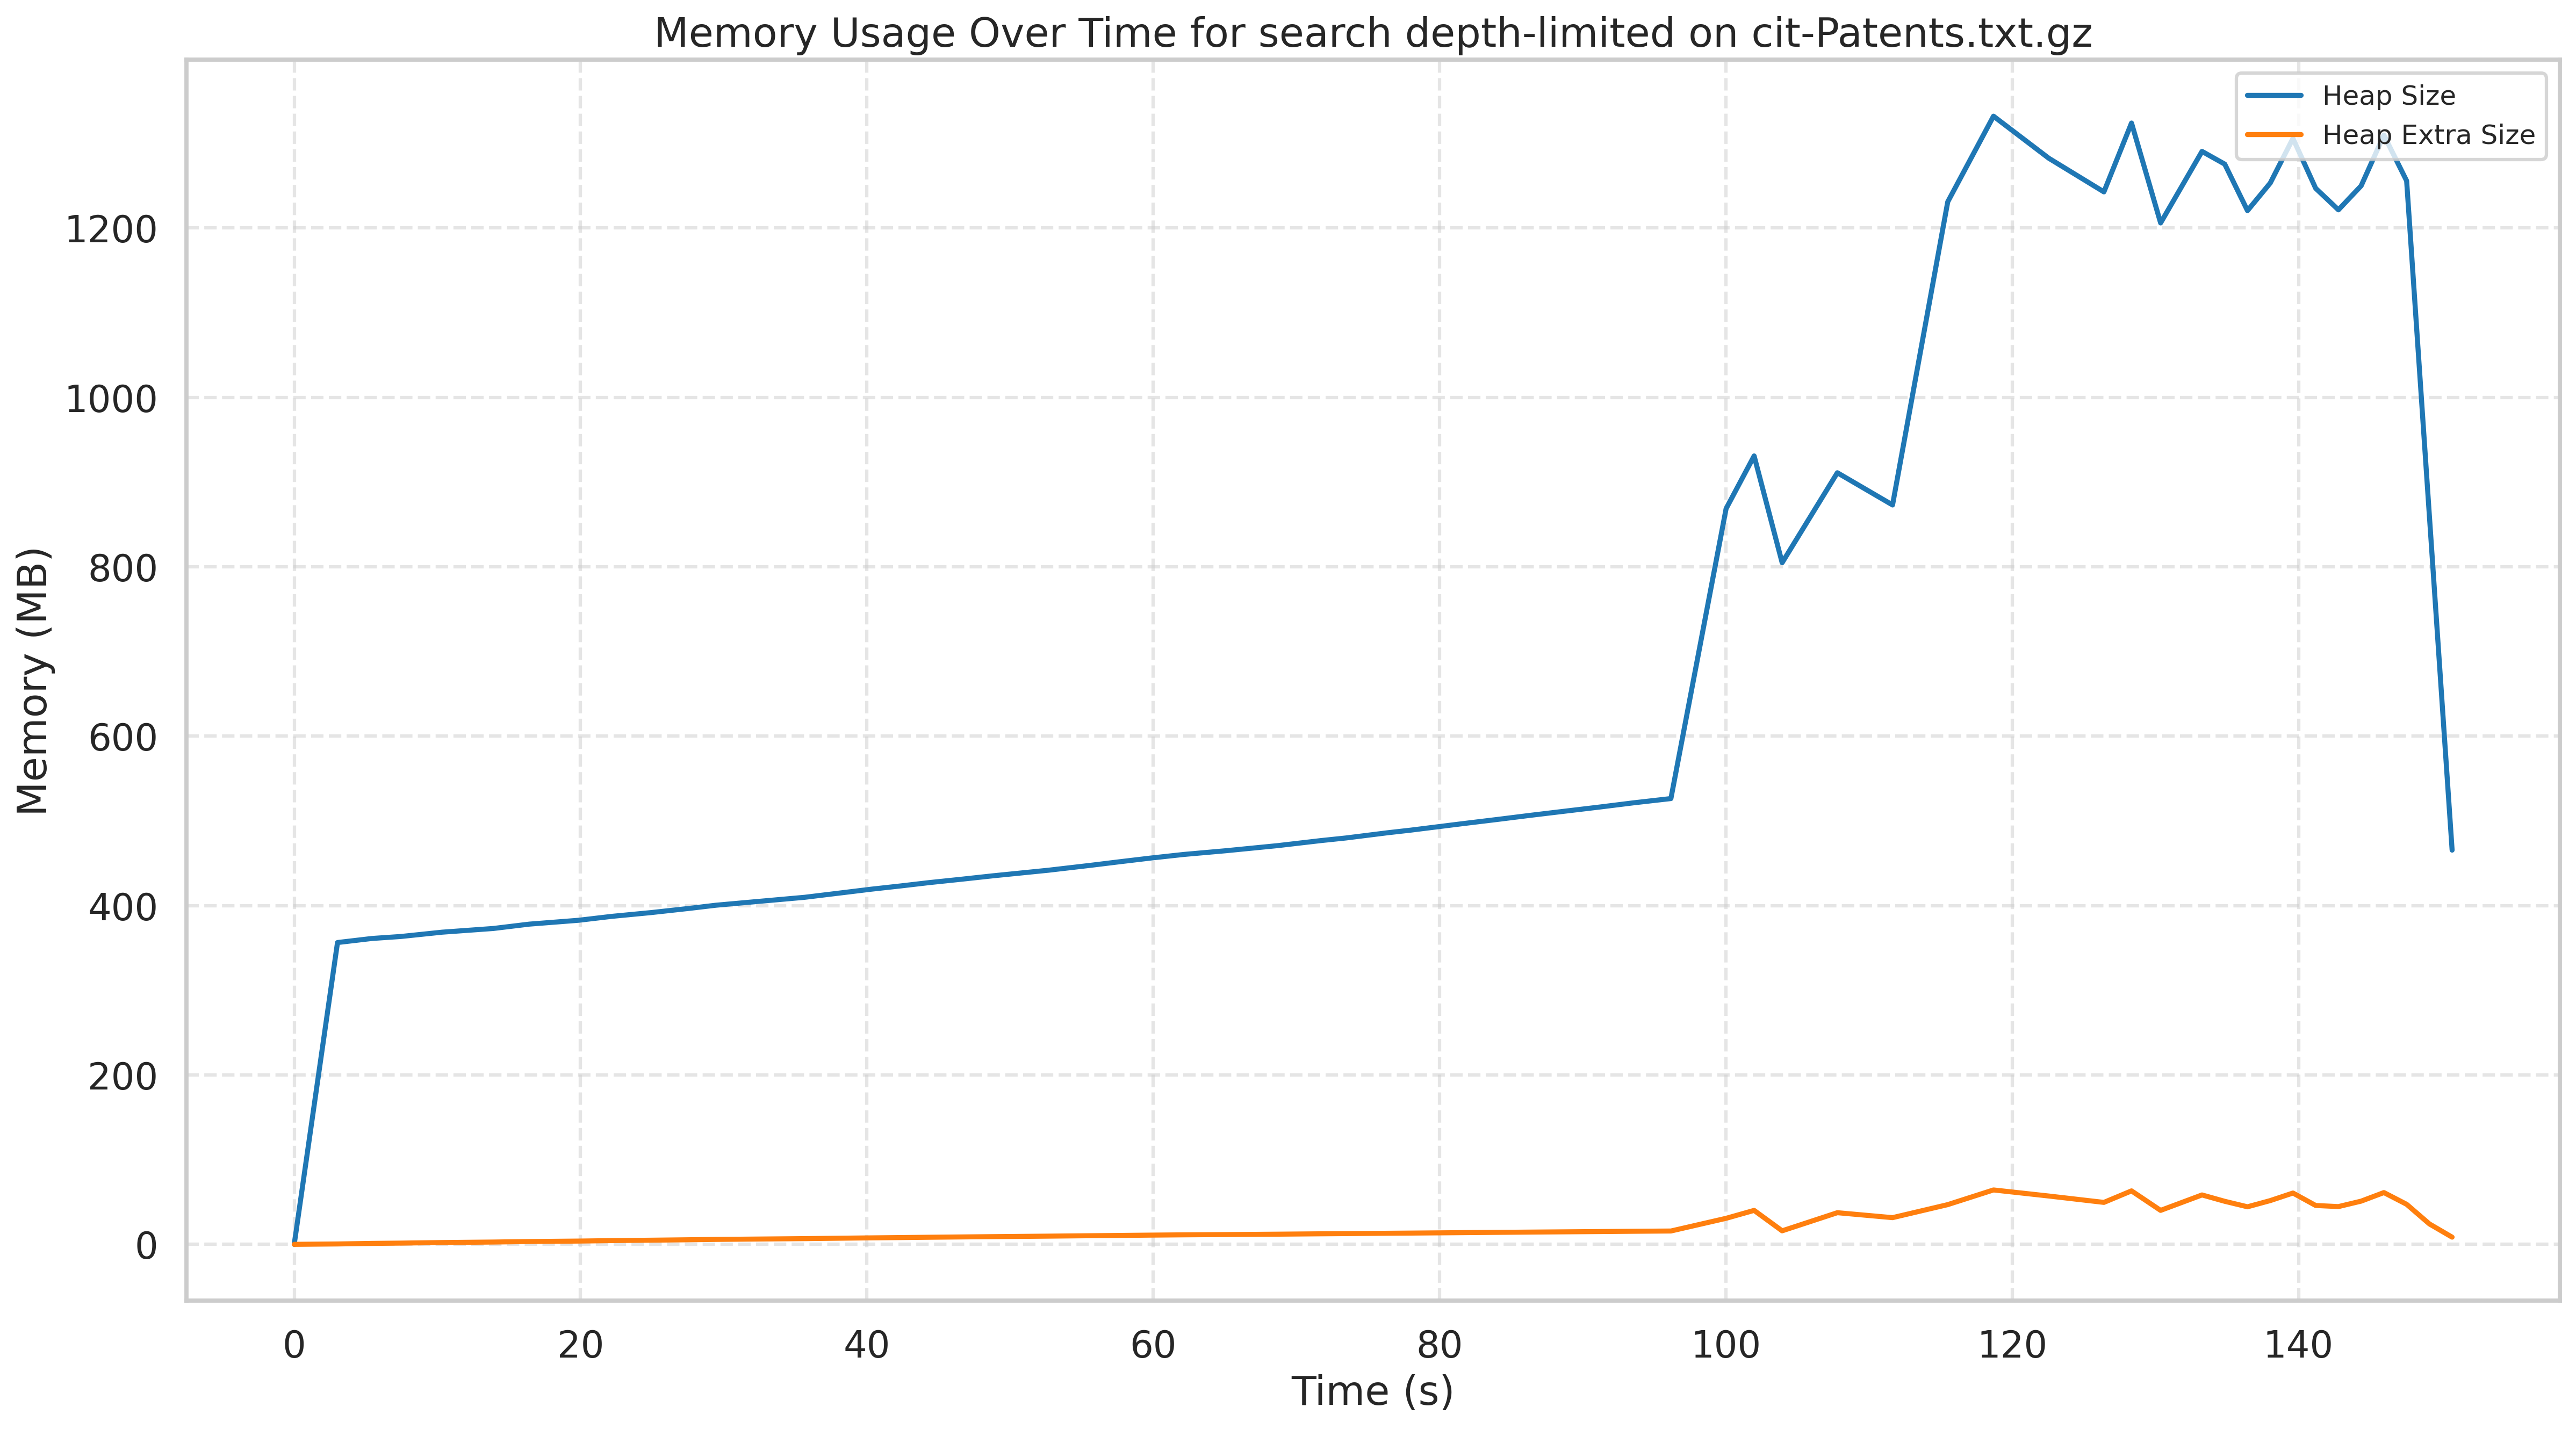
\includegraphics[width=\textwidth]{../plots/cit-Patents_depth-limited.png}
\caption{Grafico: breadth-first su com-lj.ungraph}
\end{figure}
\subsubsection{Algoritmo di ricerca: iterative-deepening}
\begin{figure}[h]\centering
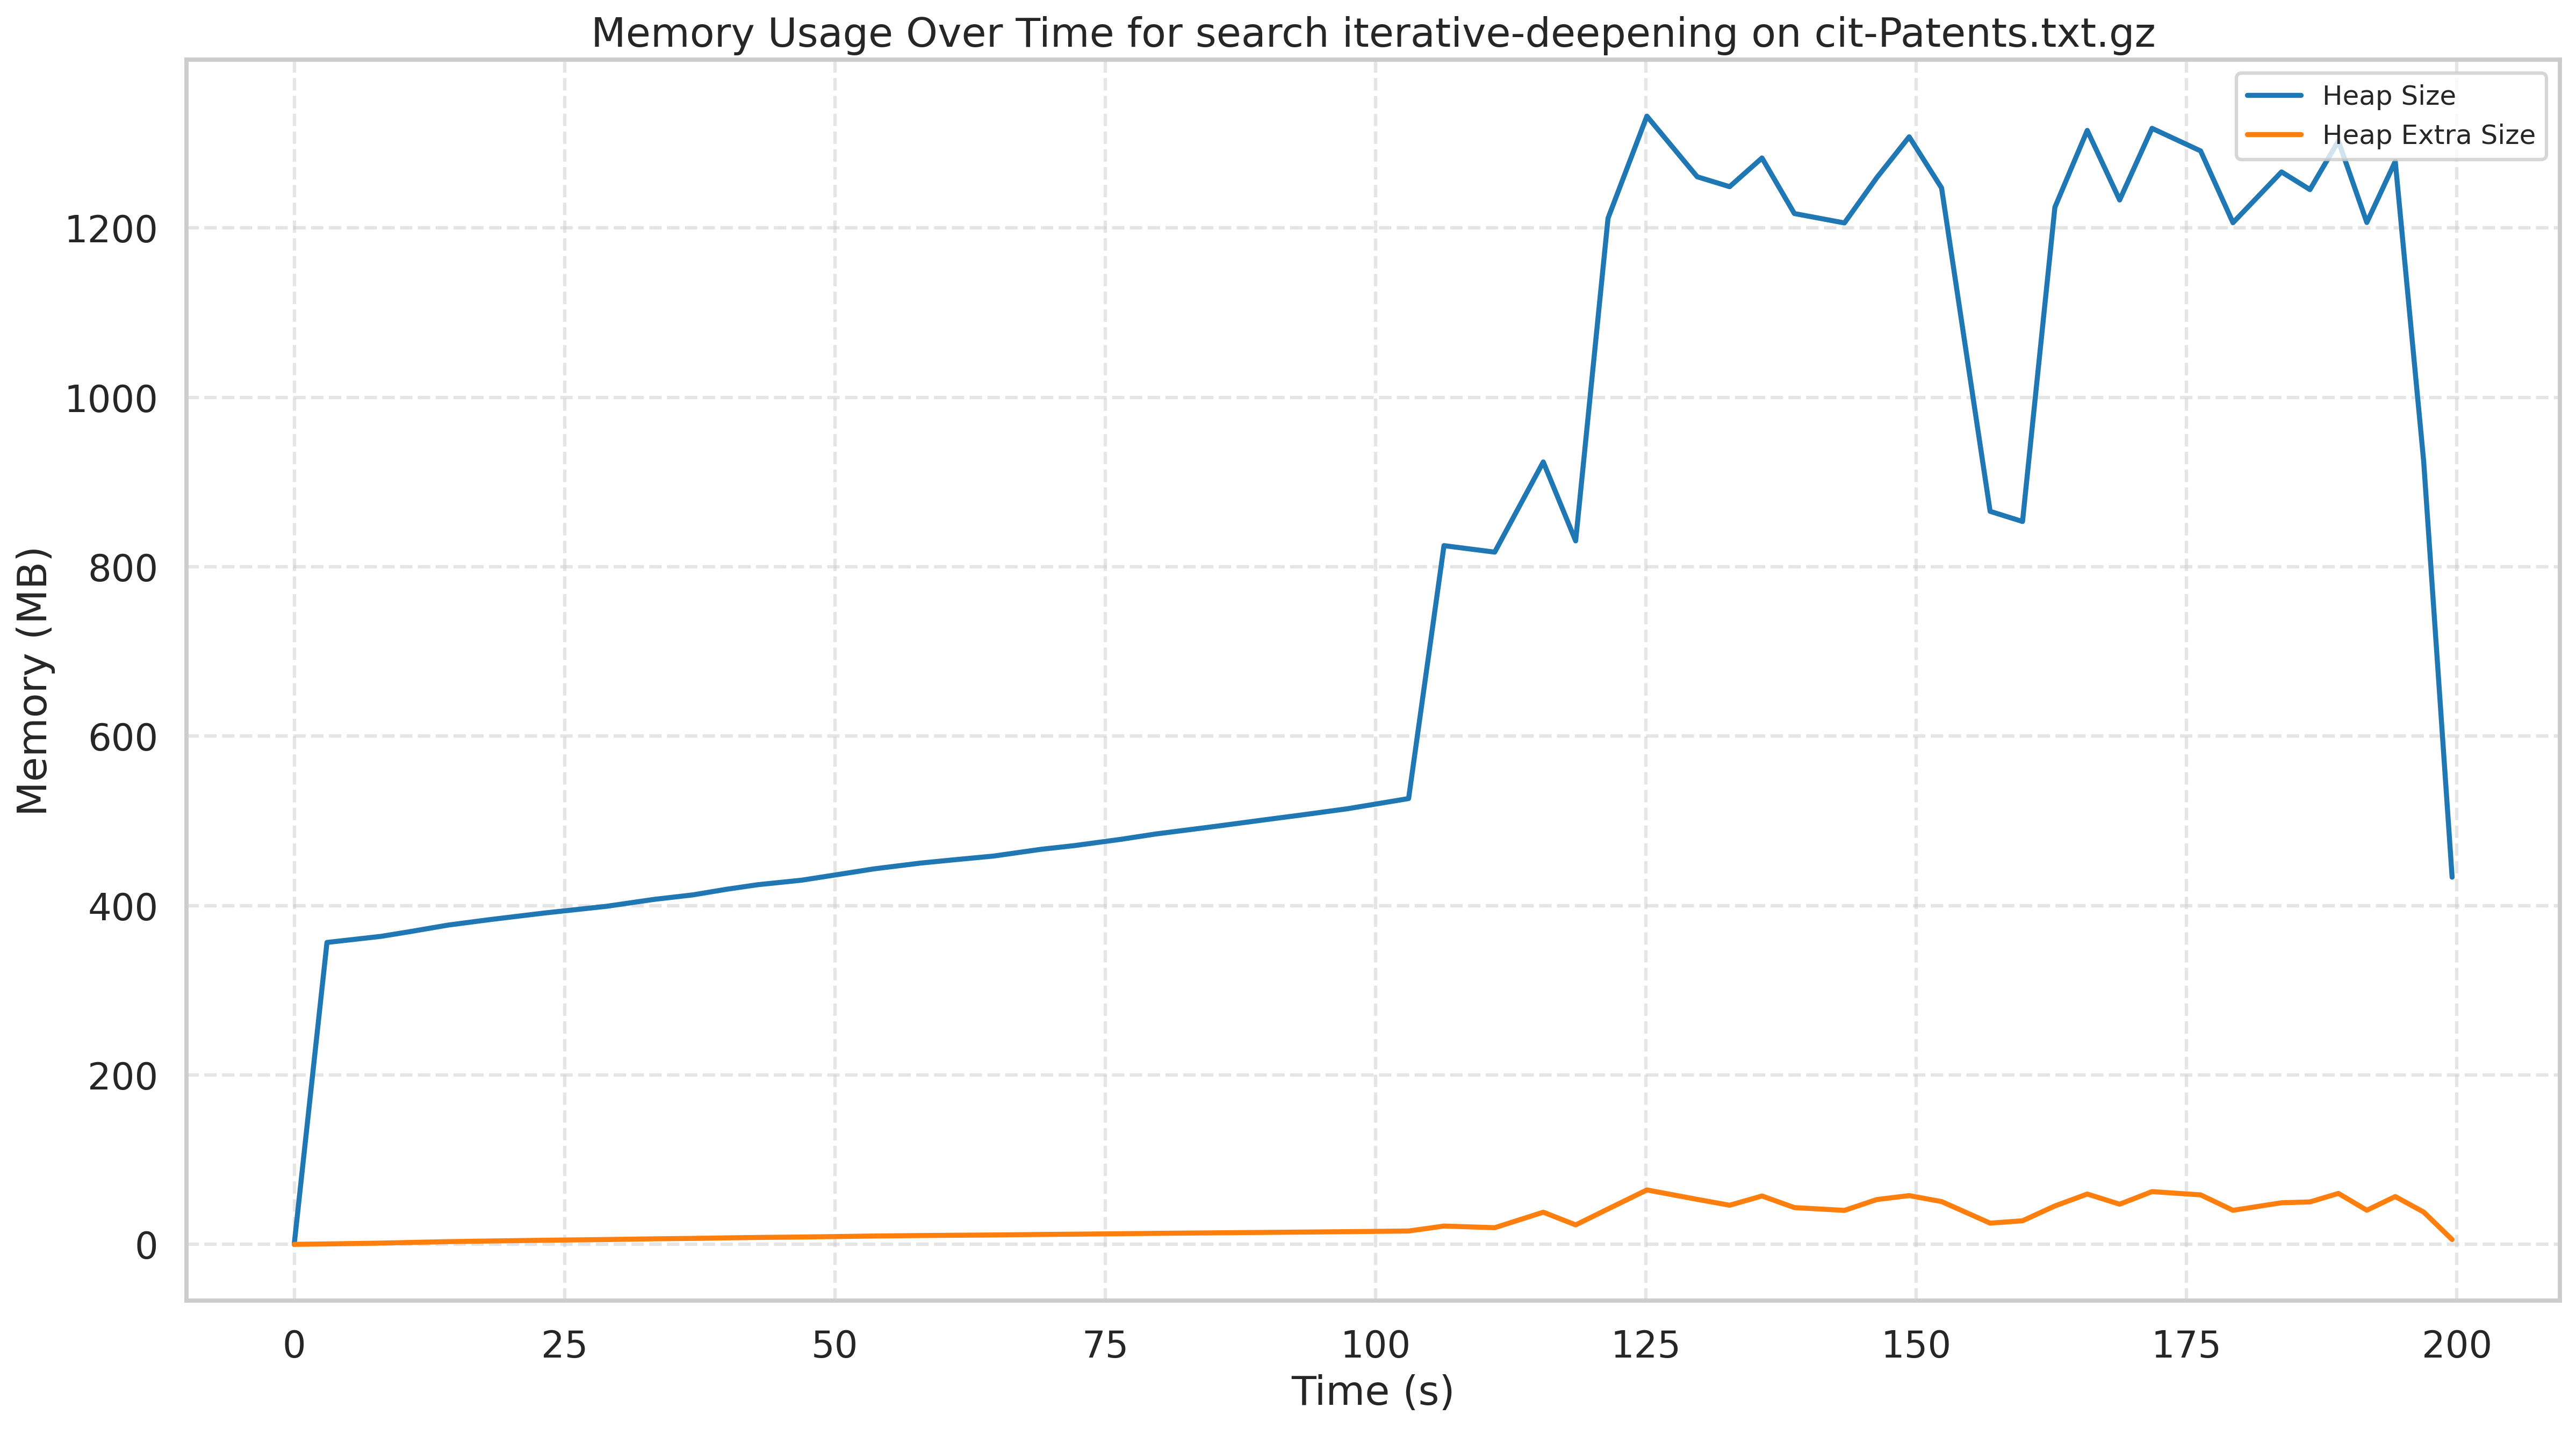
\includegraphics[width=\textwidth]{../plots/cit-Patents_iterative-deepening.png}
\caption{Grafico: breadth-first su com-lj.ungraph}
\end{figure}
\subsubsection{Algoritmo di ricerca: bi-directional}
\begin{figure}[h]\centering
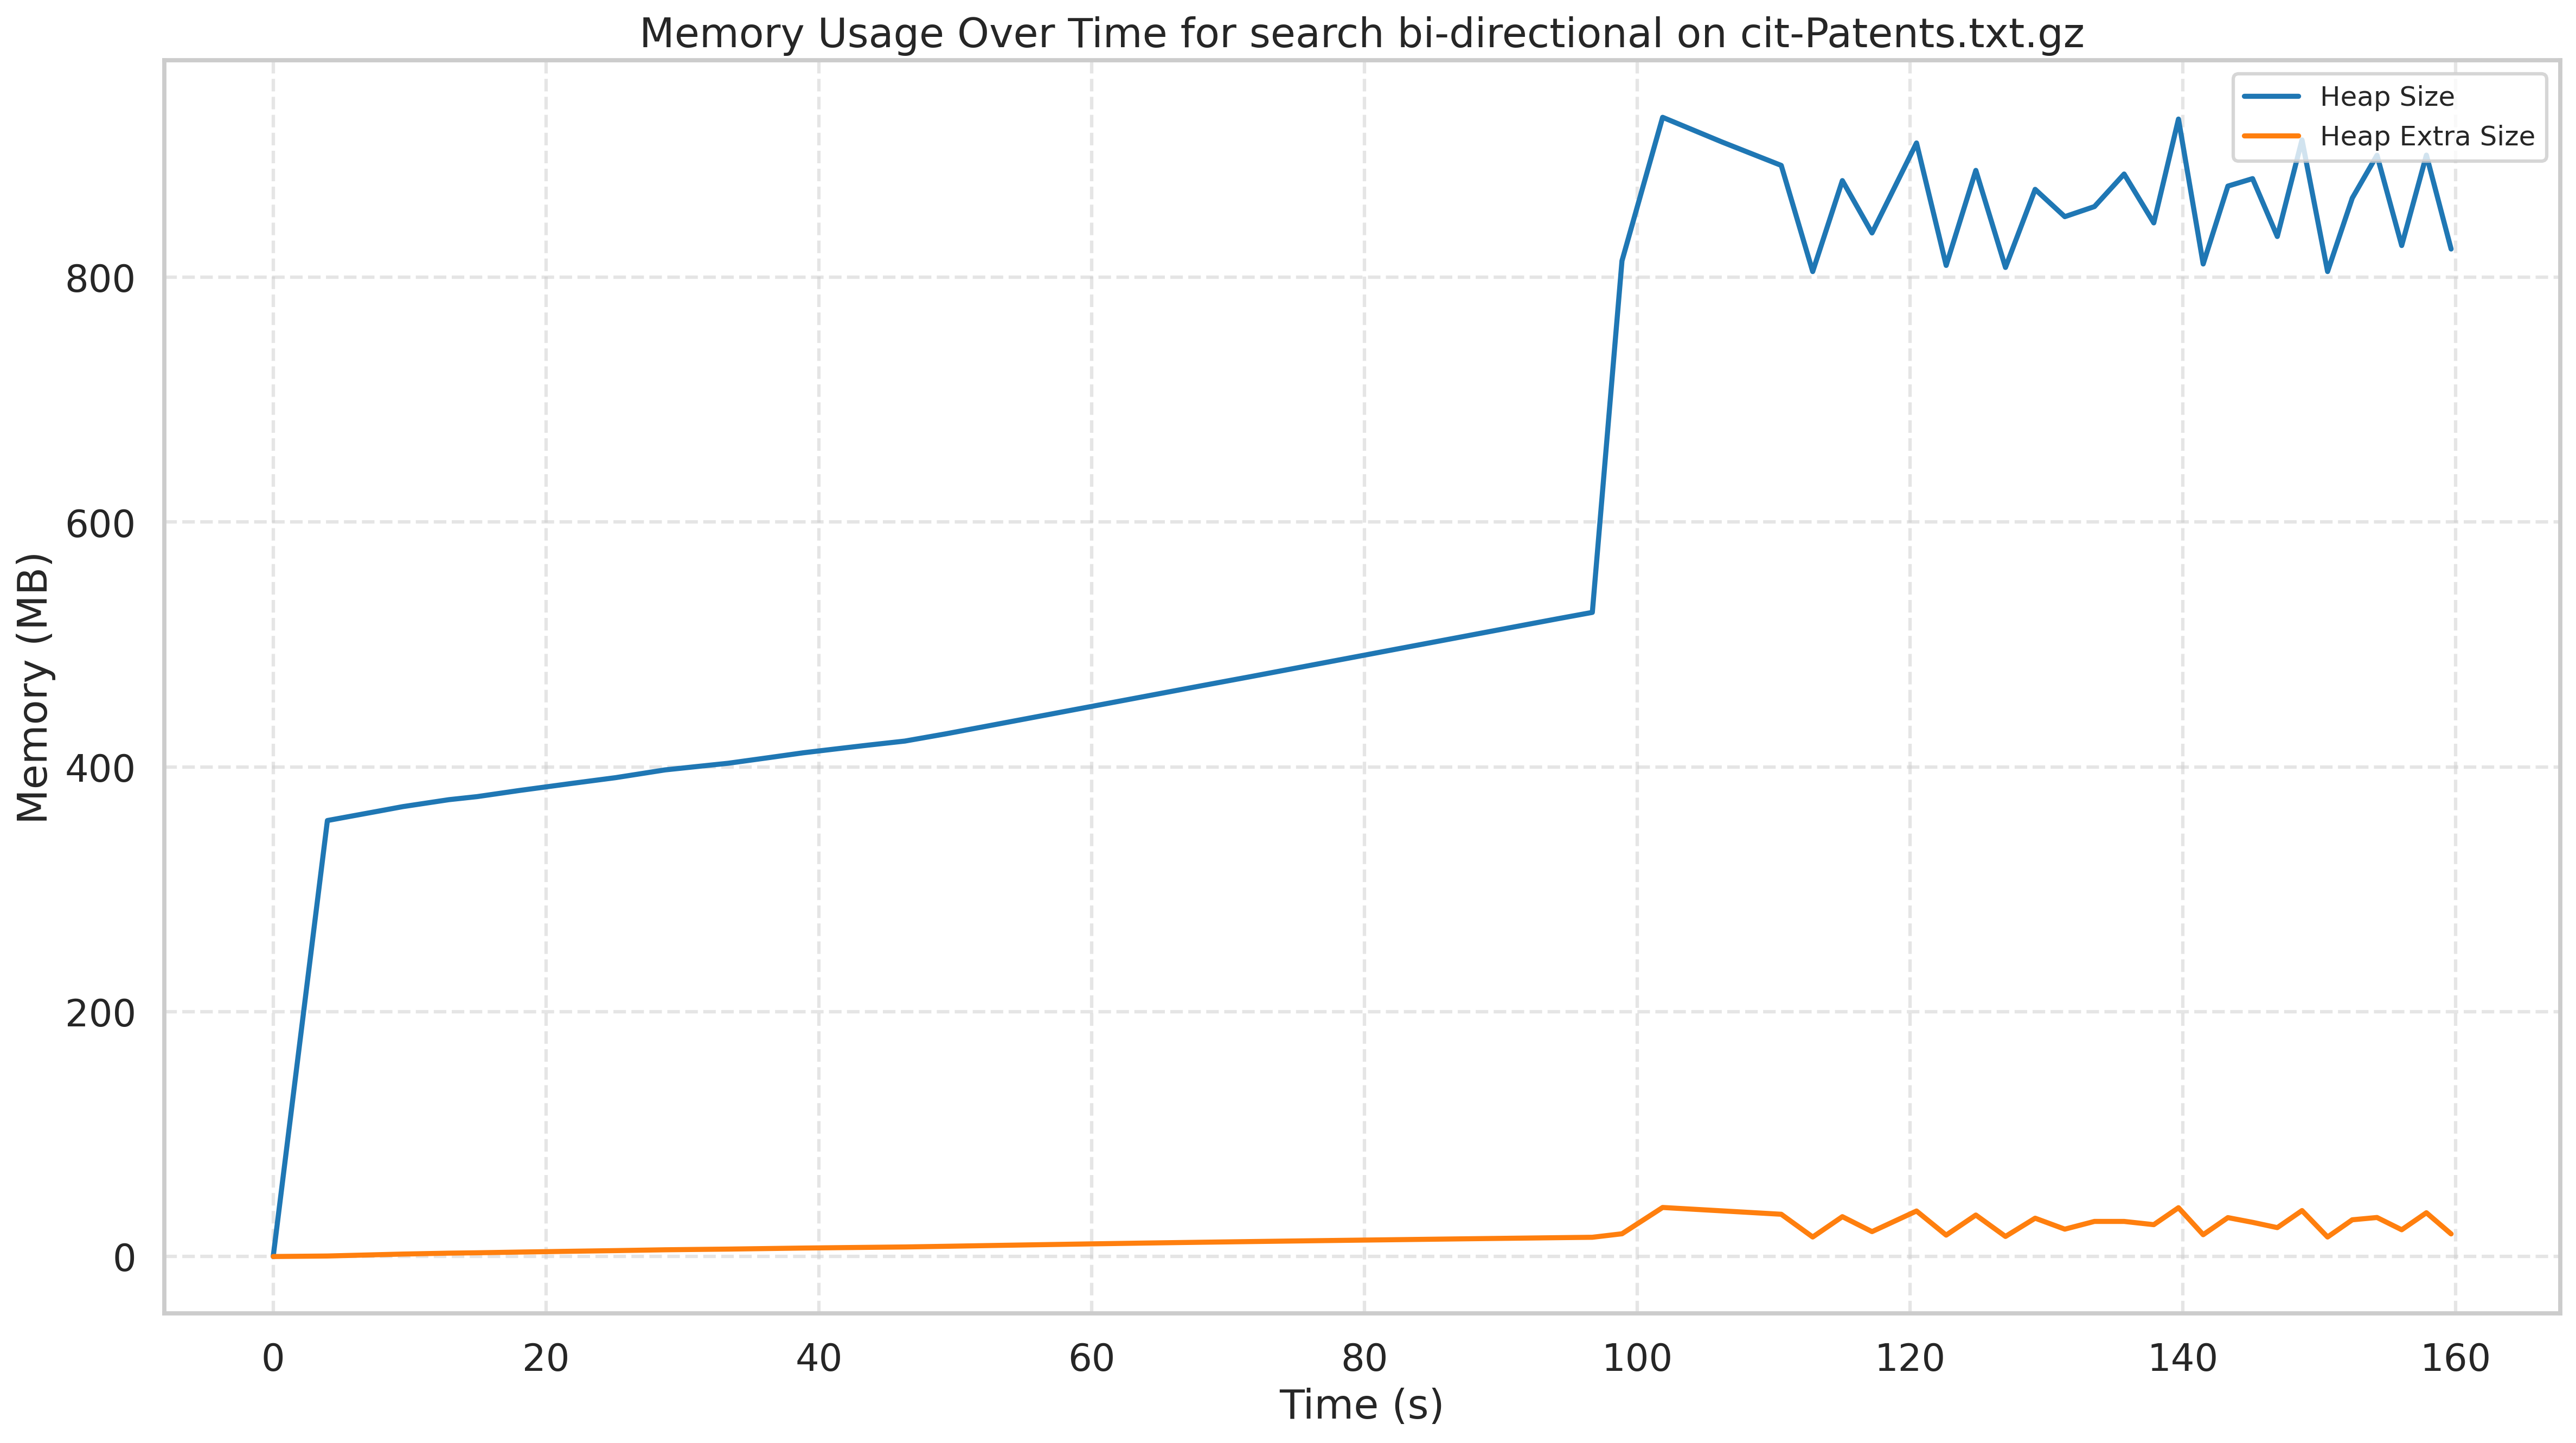
\includegraphics[width=\textwidth]{../plots/cit-Patents_bi-directional.png}
\caption{Grafico: breadth-first su com-lj.ungraph}
\end{figure}
\subsubsection{Algoritmo di ricerca: breadth-first}
\begin{figure}[h]\centering
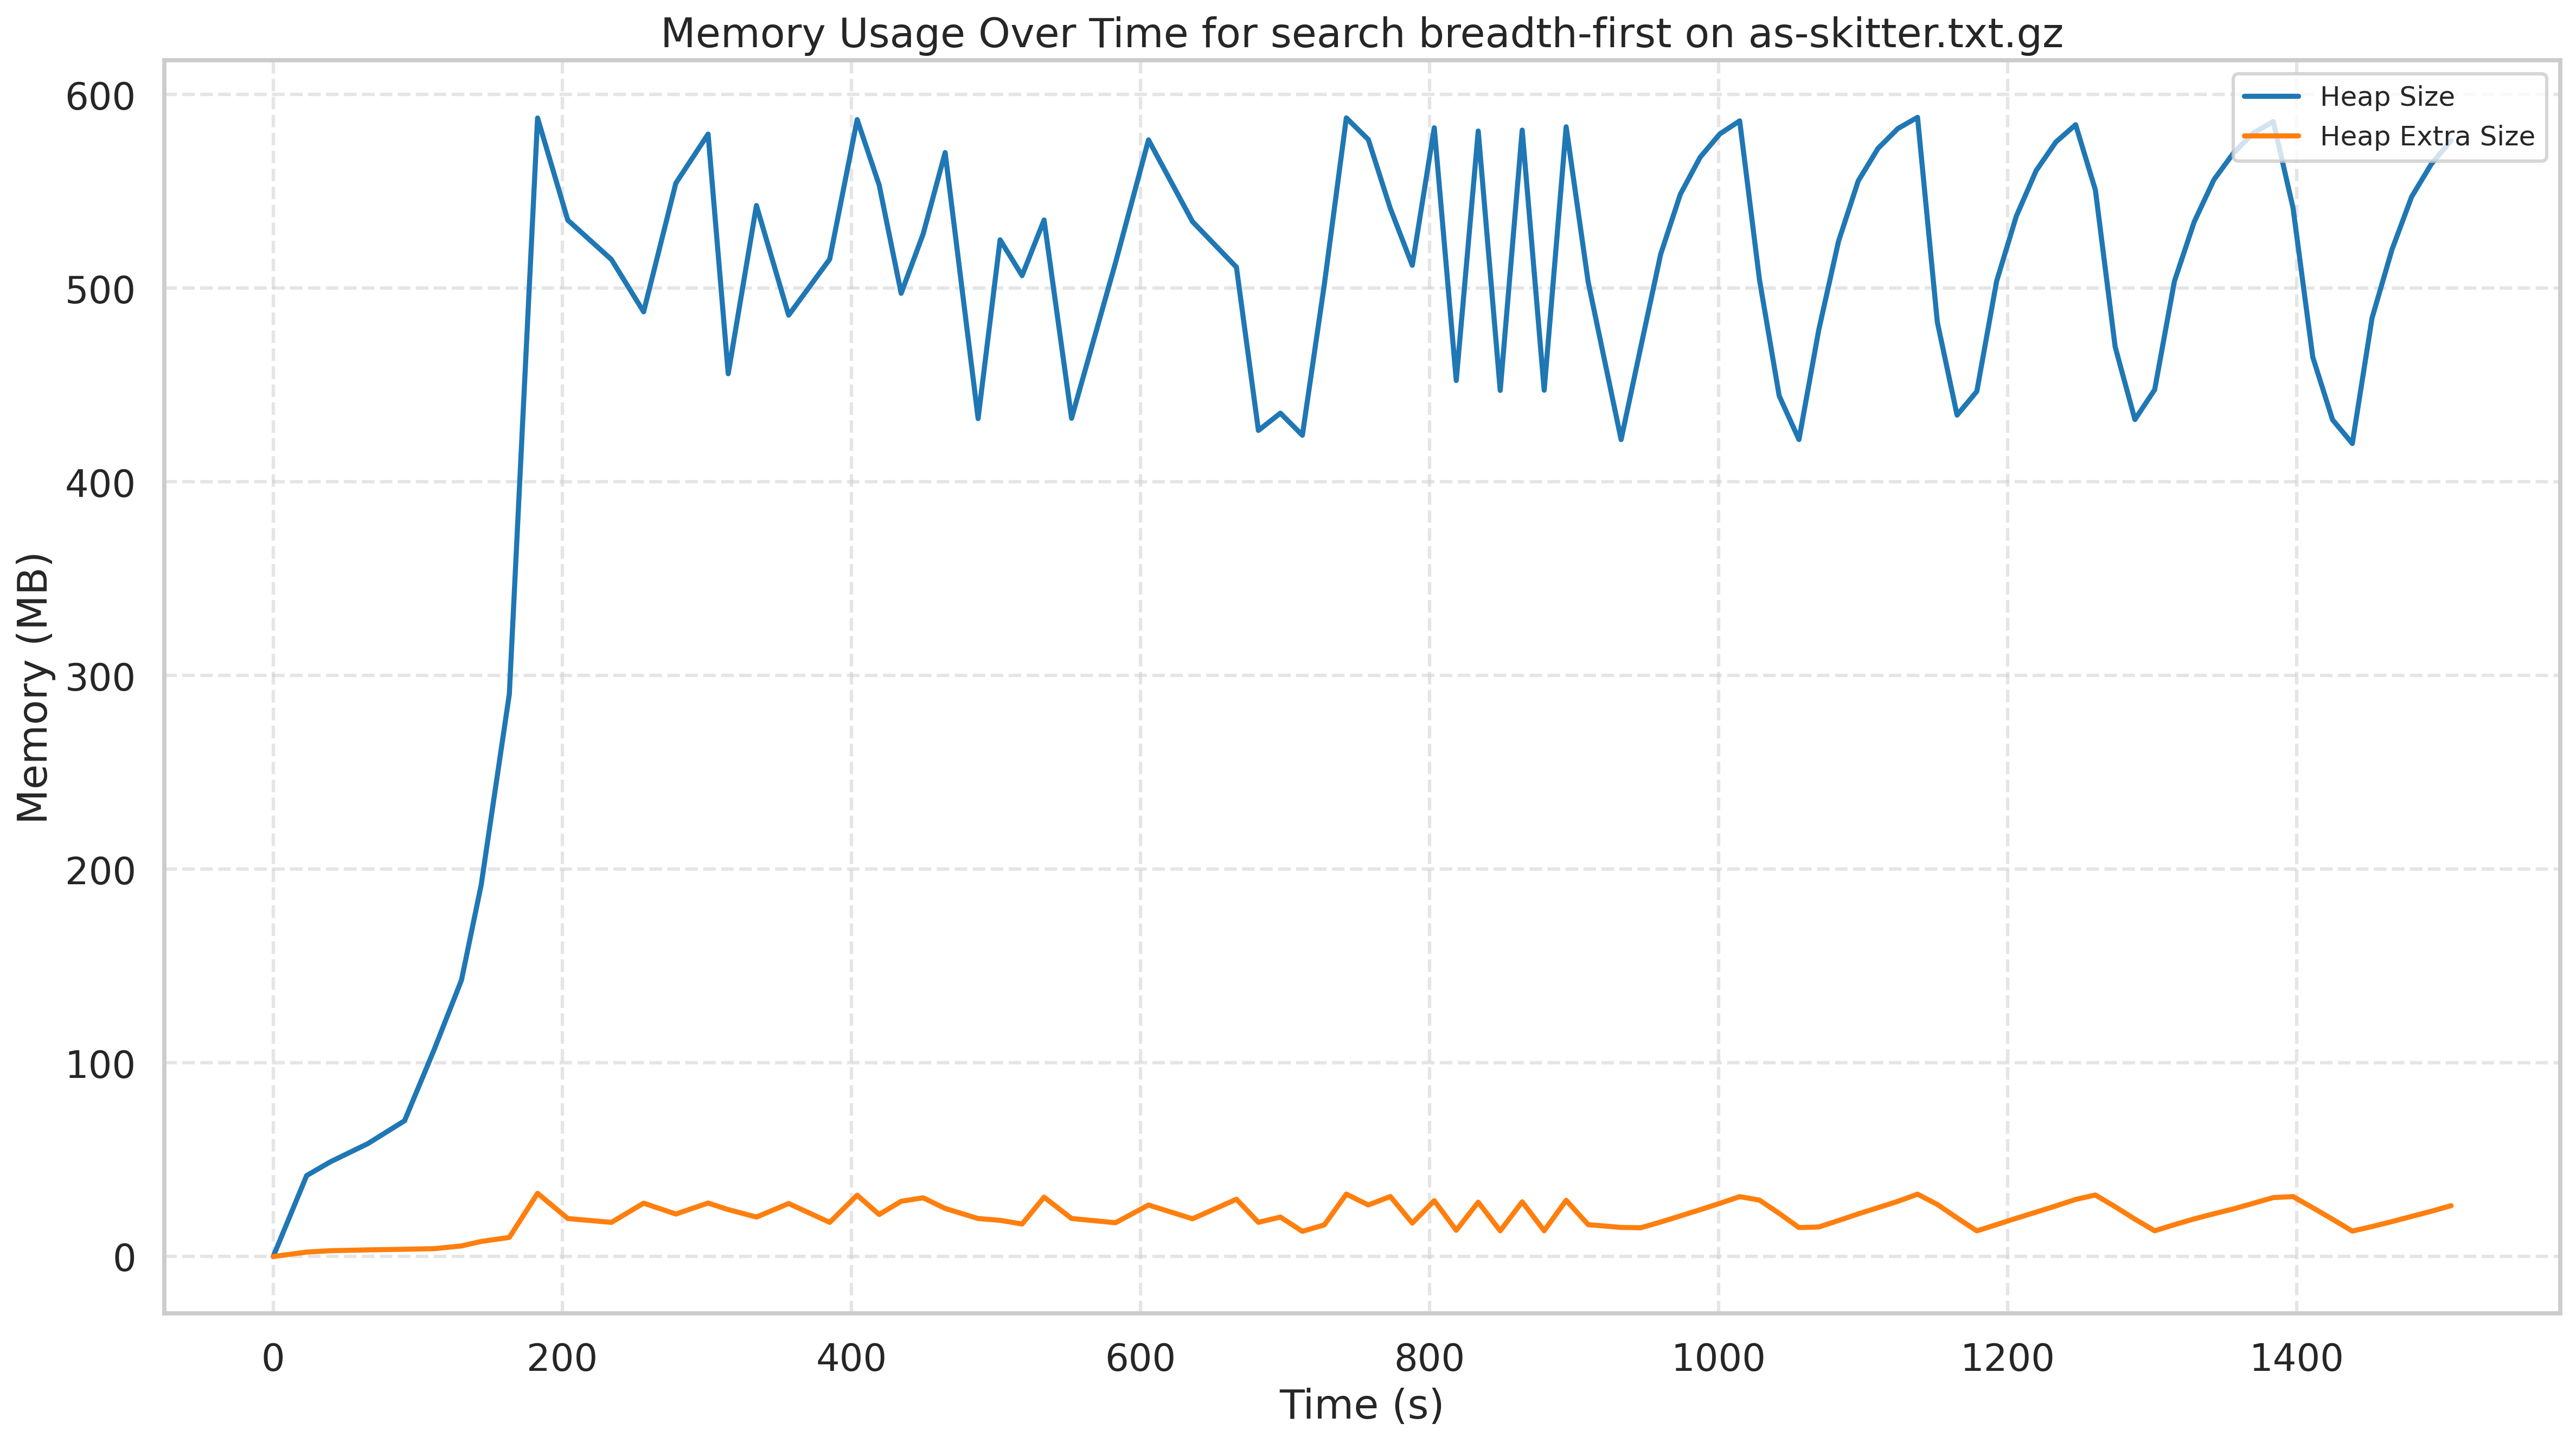
\includegraphics[width=\textwidth]{../plots/as-skitter_breadth-first.png}
\caption{Grafico: breadth-first su com-lj.ungraph}
\end{figure}
\subsubsection{Algoritmo di ricerca: uniform-cost}
\begin{figure}[h]\centering
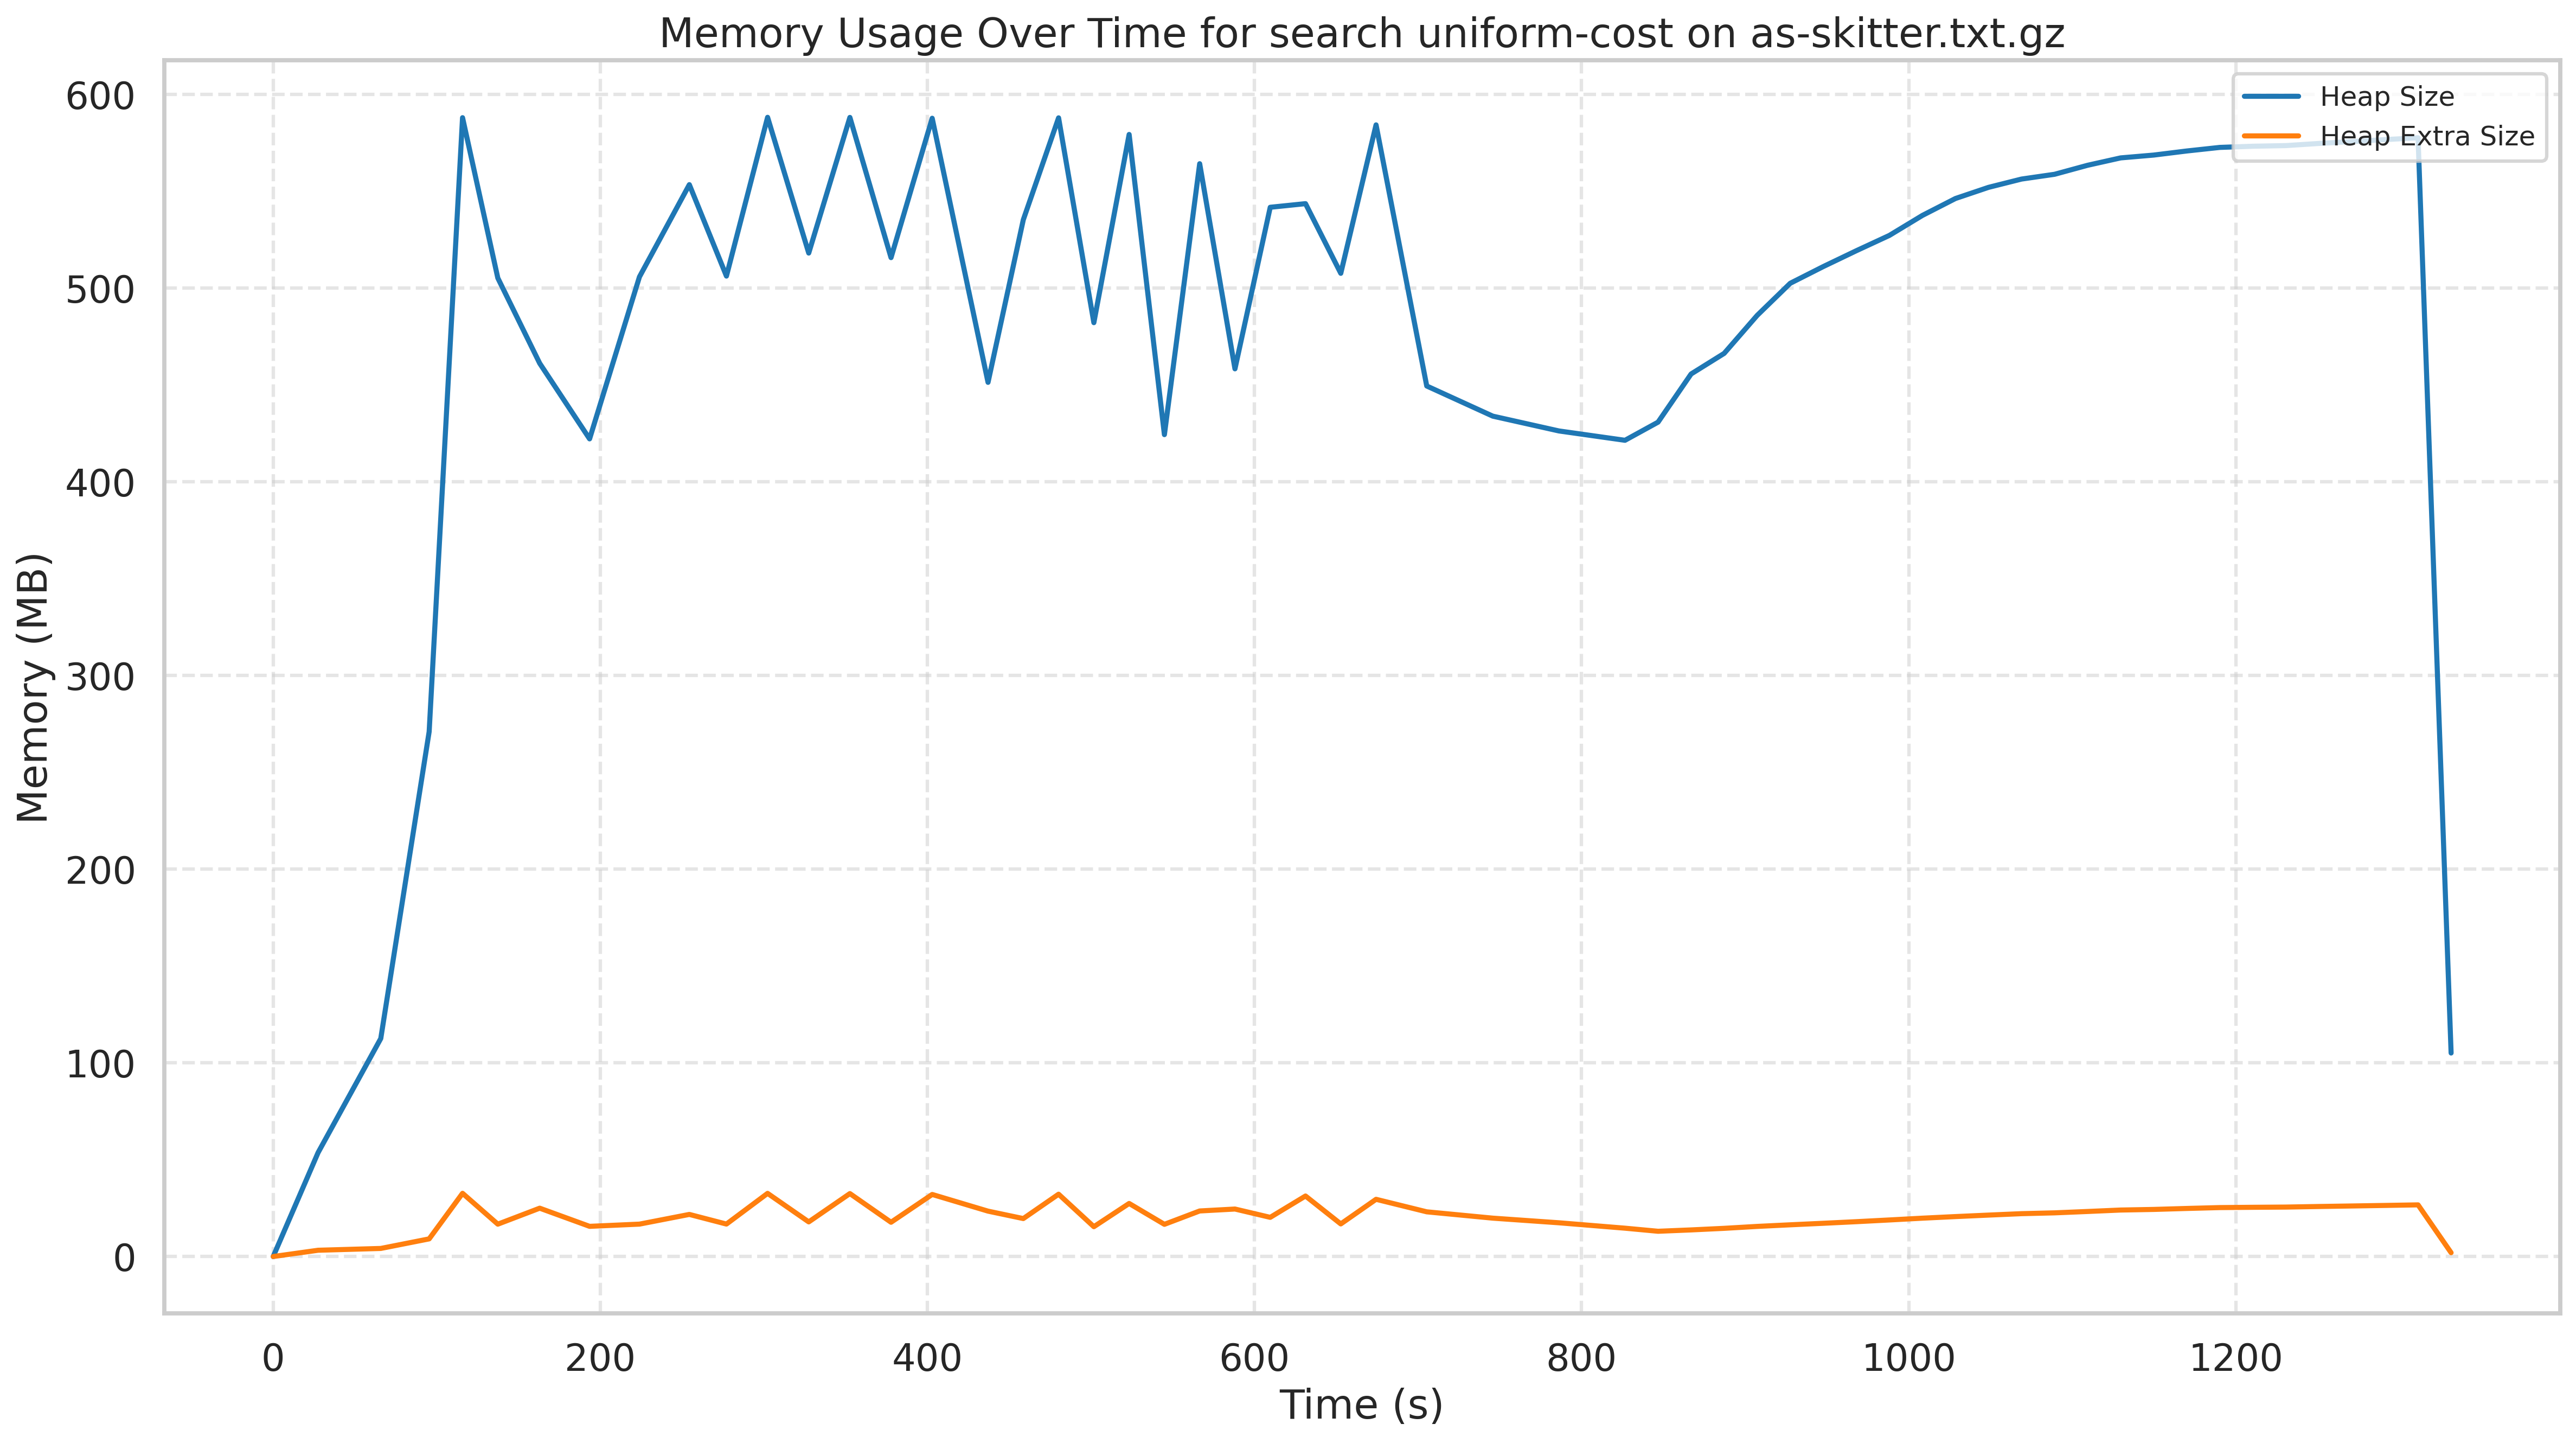
\includegraphics[width=\textwidth]{../plots/as-skitter_uniform-cost.png}
\caption{Grafico: breadth-first su com-lj.ungraph}
\end{figure}
\subsubsection{Algoritmo di ricerca: depth-limited}
\begin{figure}[h]\centering
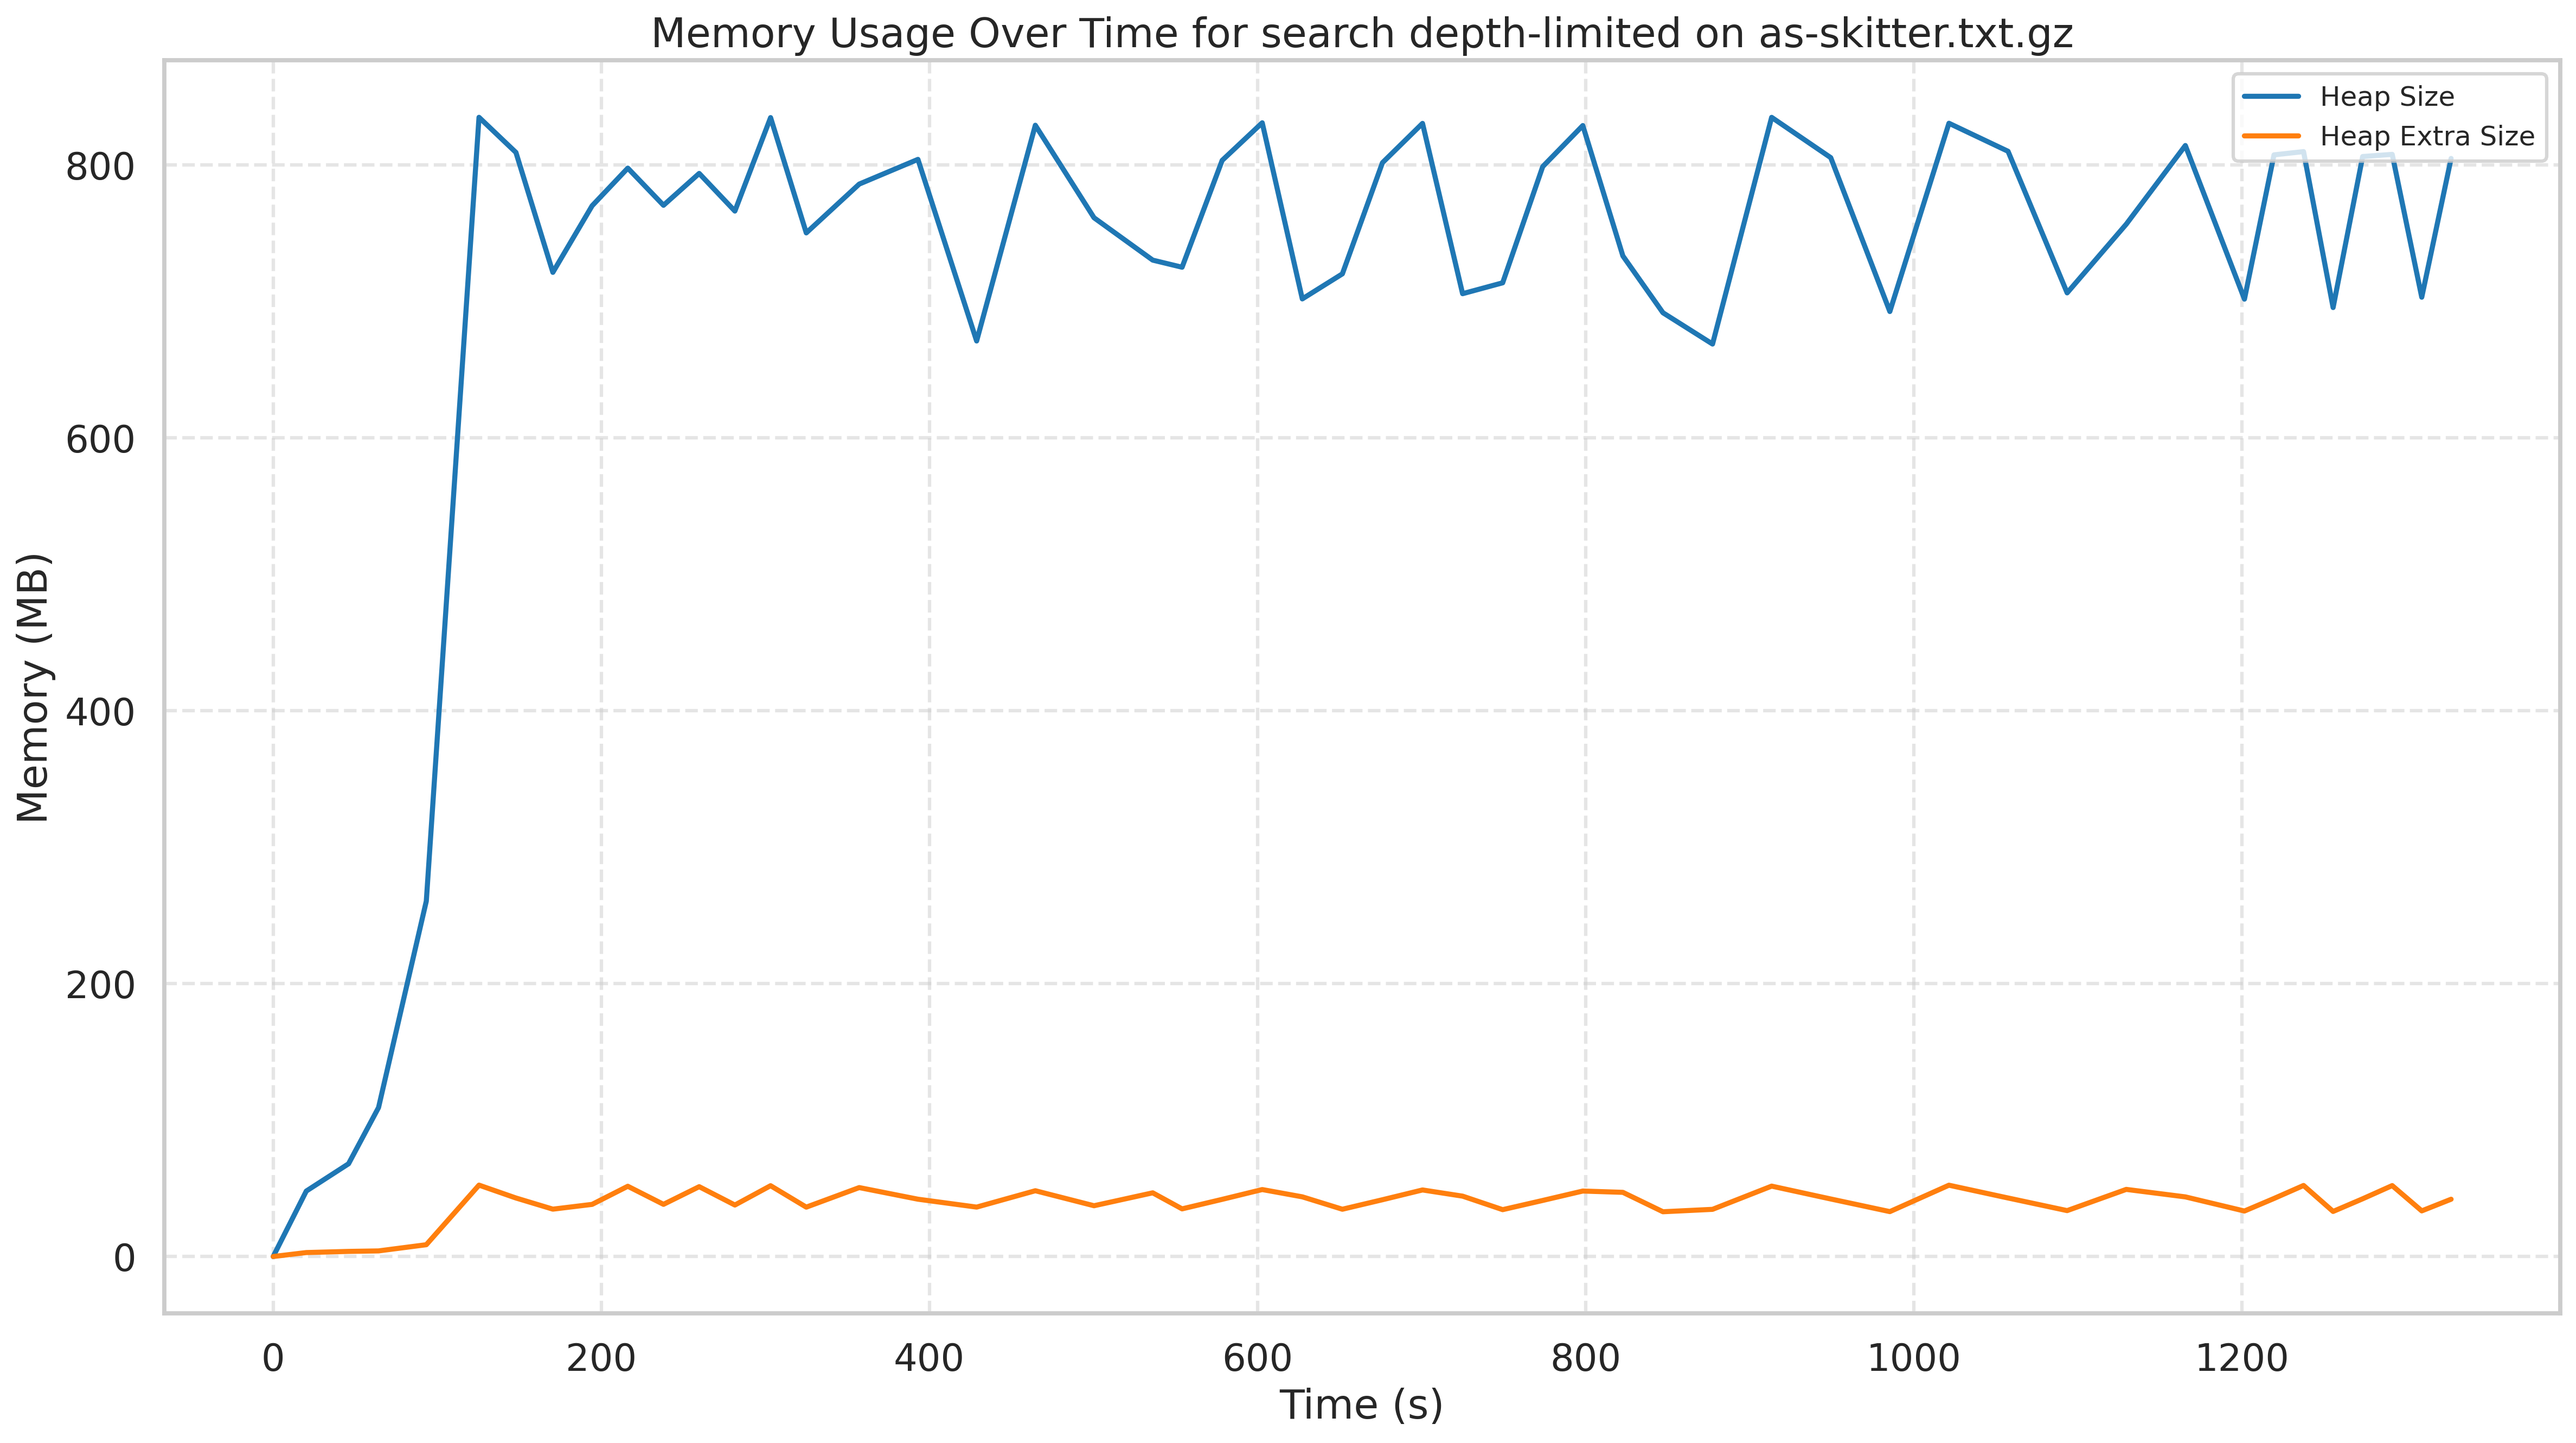
\includegraphics[width=\textwidth]{../plots/as-skitter_depth-limited.png}
\caption{Grafico: breadth-first su com-lj.ungraph}
\end{figure}
\subsubsection{Algoritmo di ricerca: iterative-deepening}
\begin{figure}[h]\centering
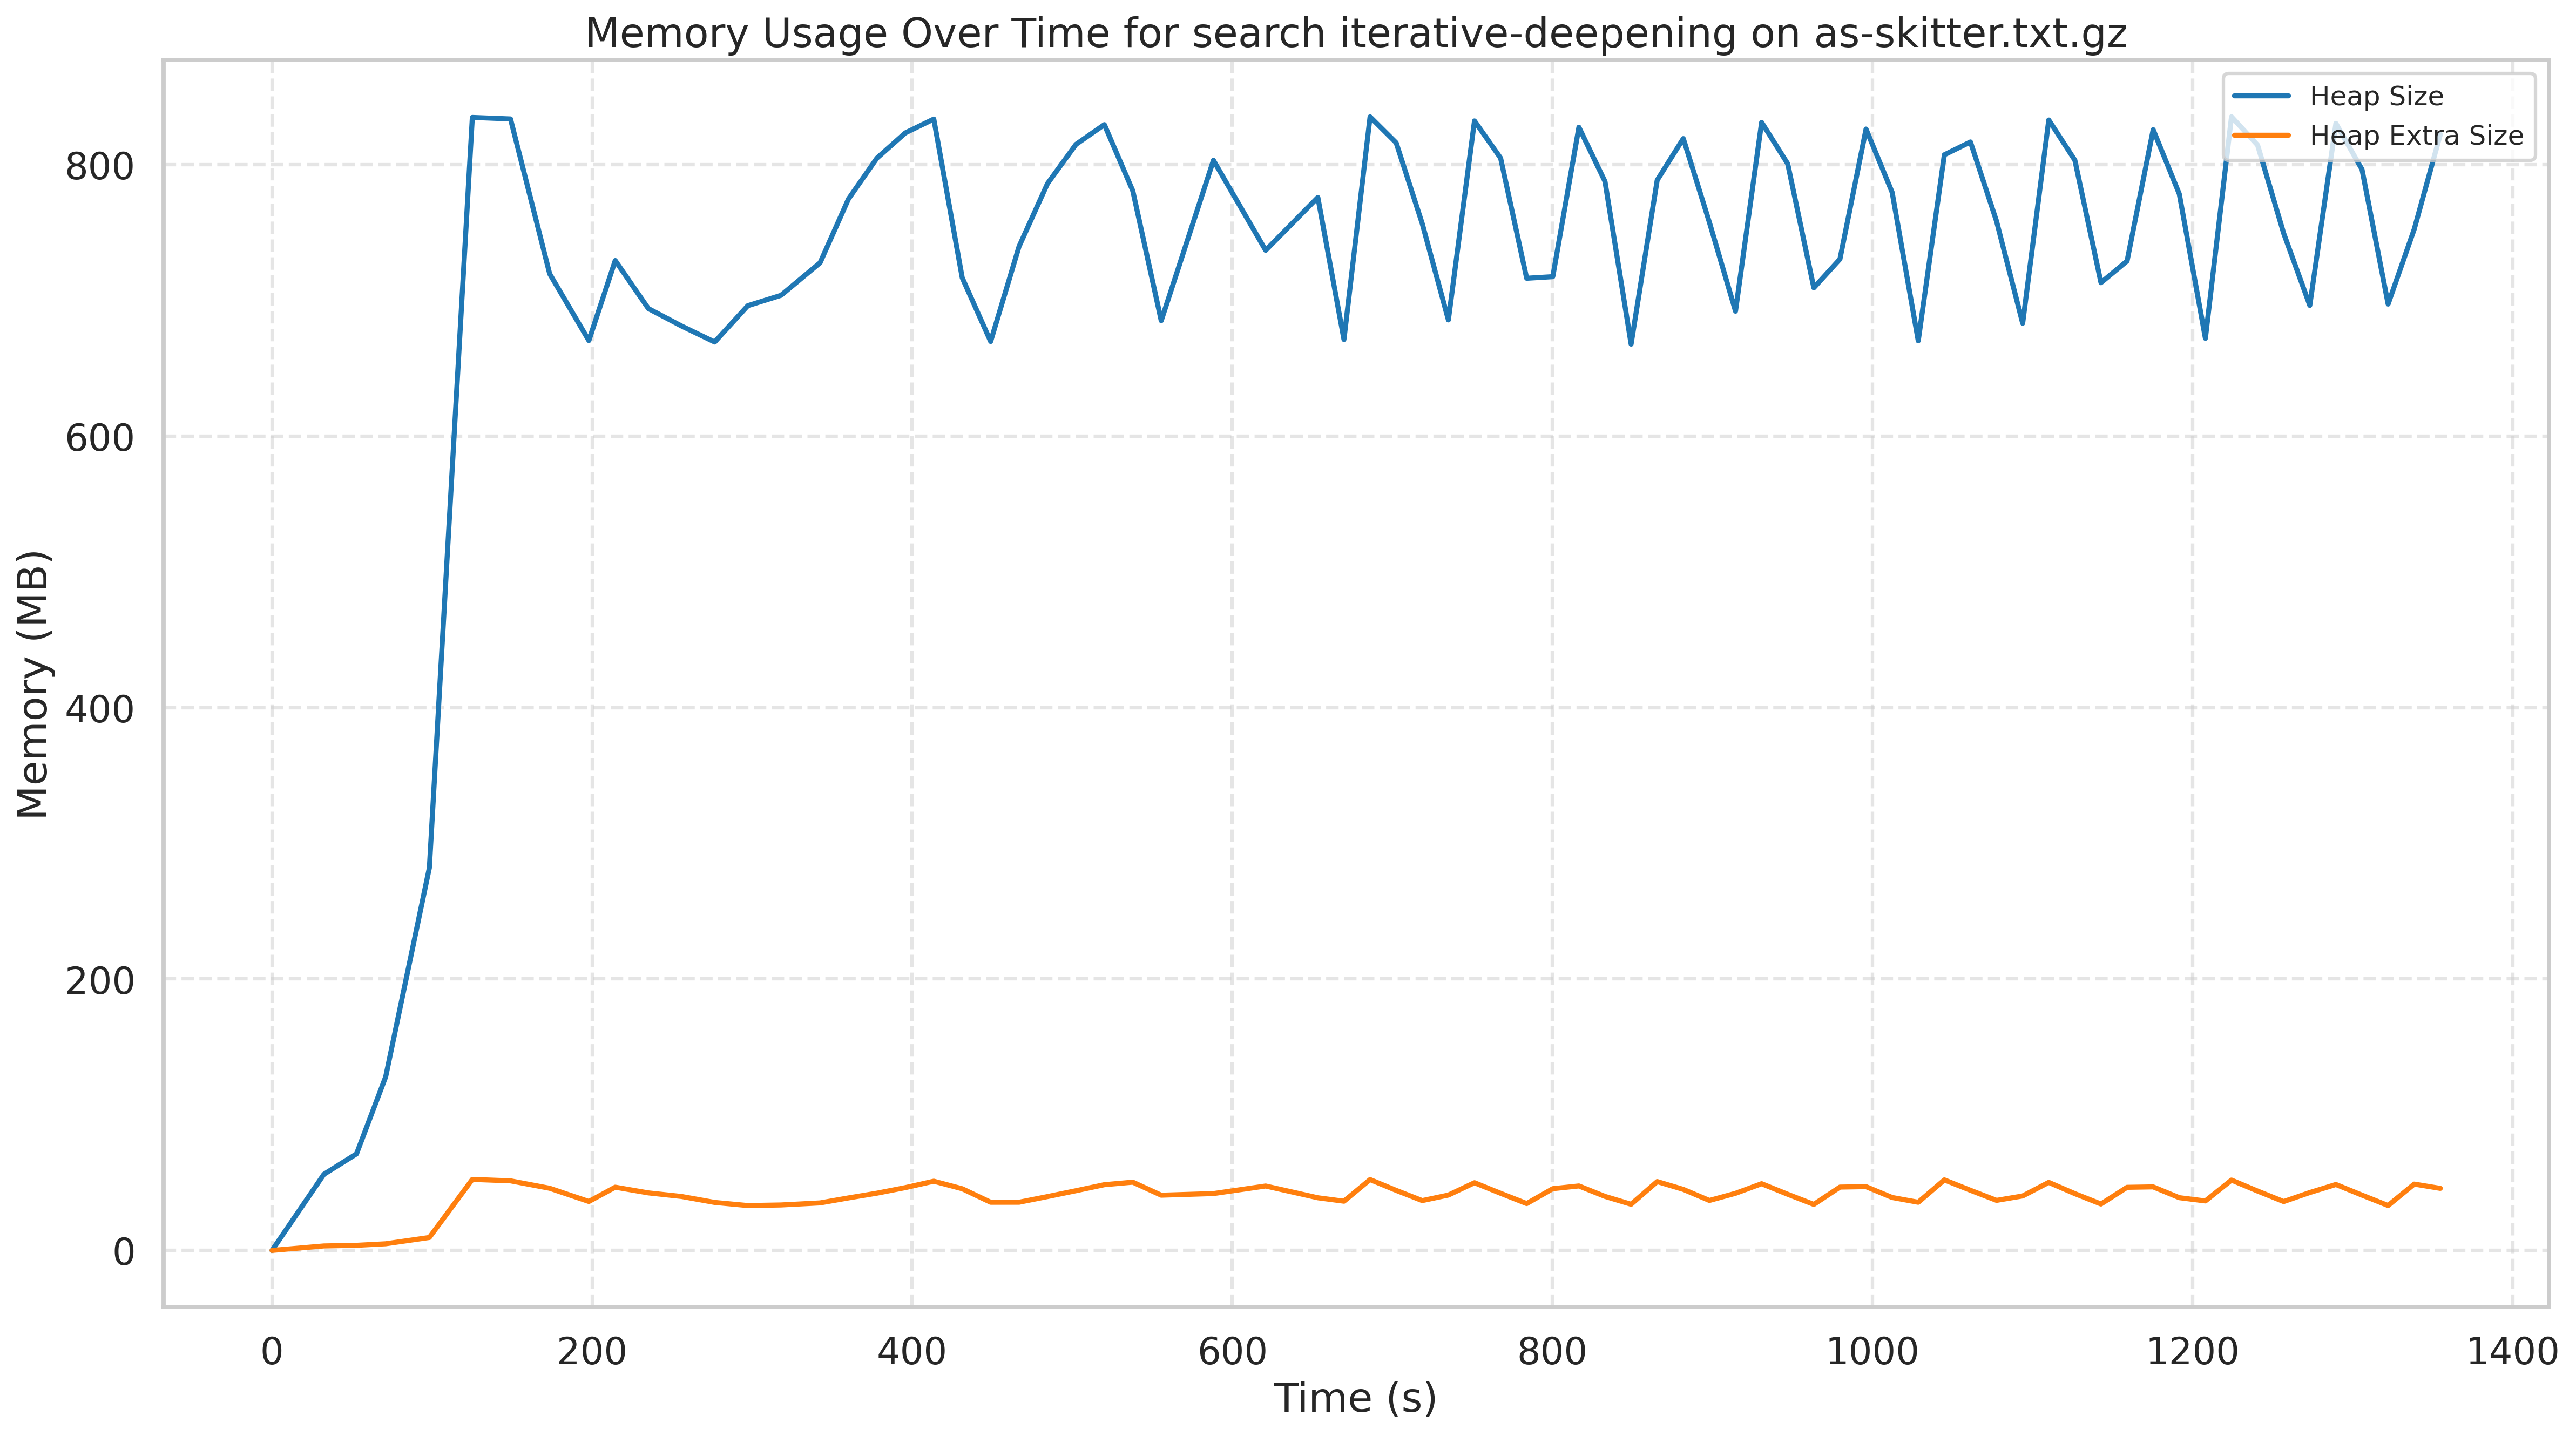
\includegraphics[width=\textwidth]{../plots/as-skitter_iterative-deepening.png}
\caption{Grafico: breadth-first su com-lj.ungraph}
\end{figure}
\subsubsection{Algoritmo di ricerca: bi-directional}
\begin{figure}[h]\centering
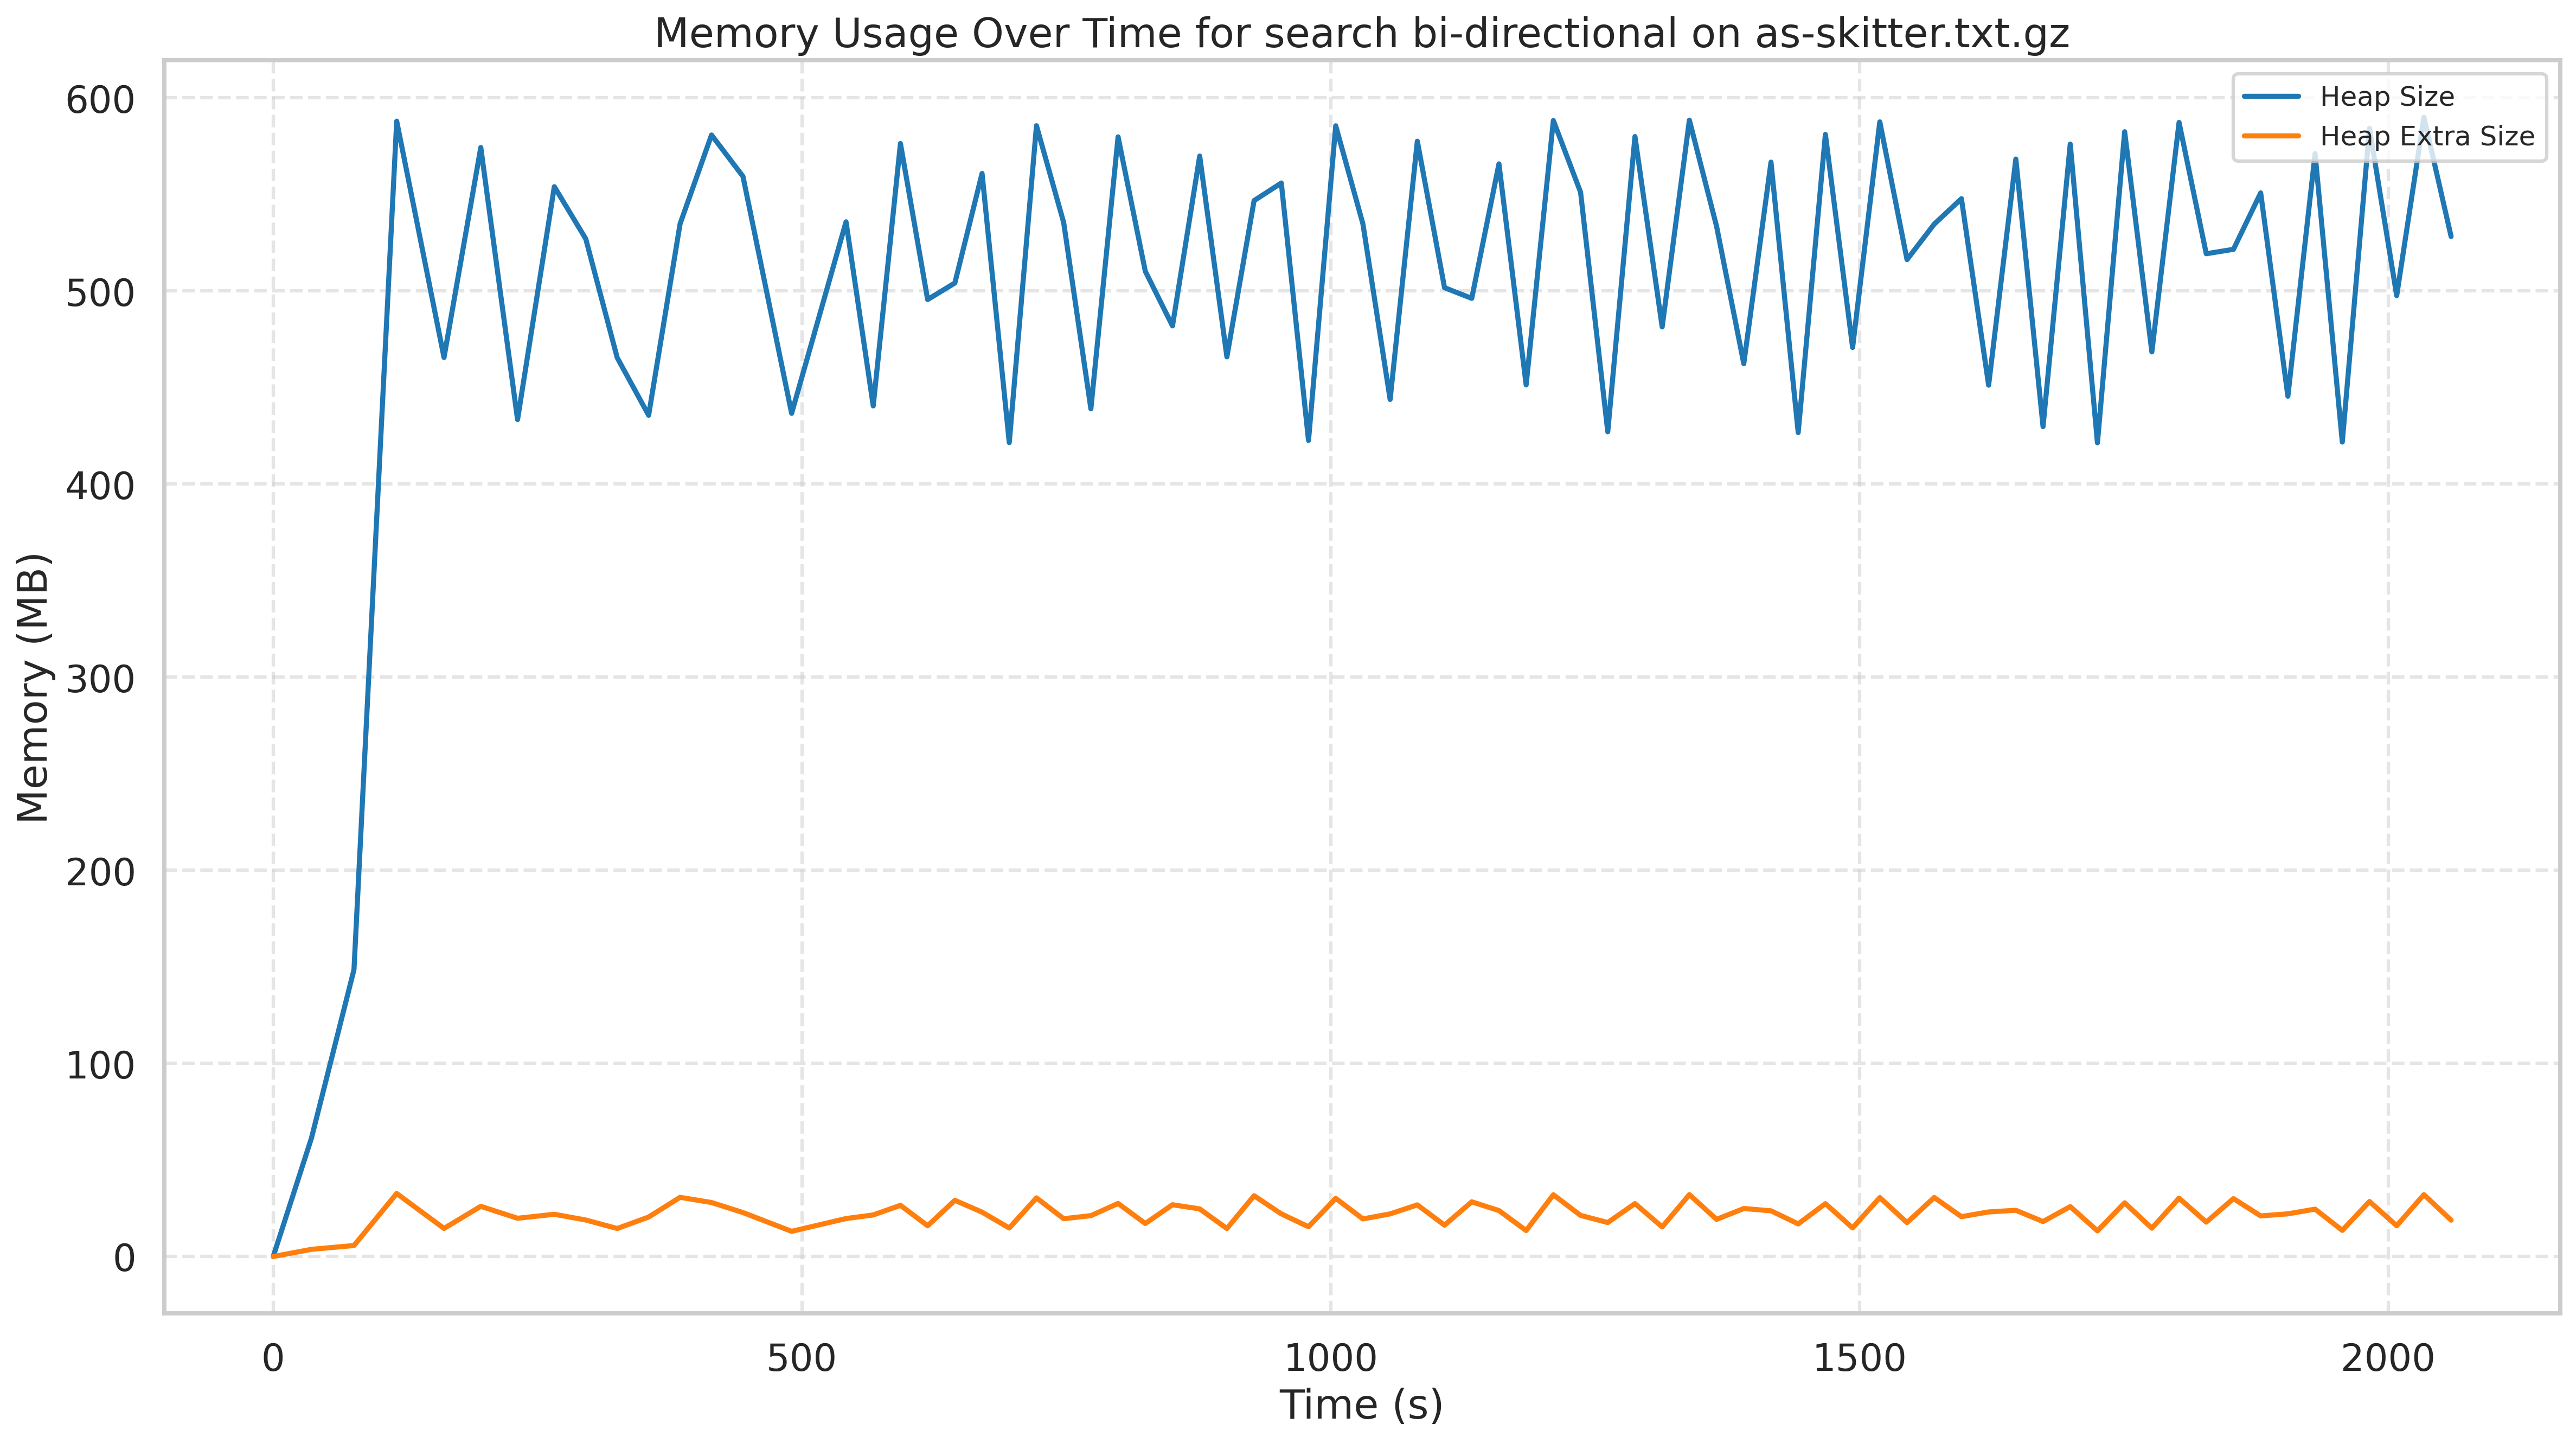
\includegraphics[width=\textwidth]{../plots/as-skitter_bi-directional.png}
\caption{Grafico: breadth-first su com-lj.ungraph}
\end{figure}
\subsubsection{Algoritmo di ricerca: breadth-first}
\begin{figure}[h]\centering
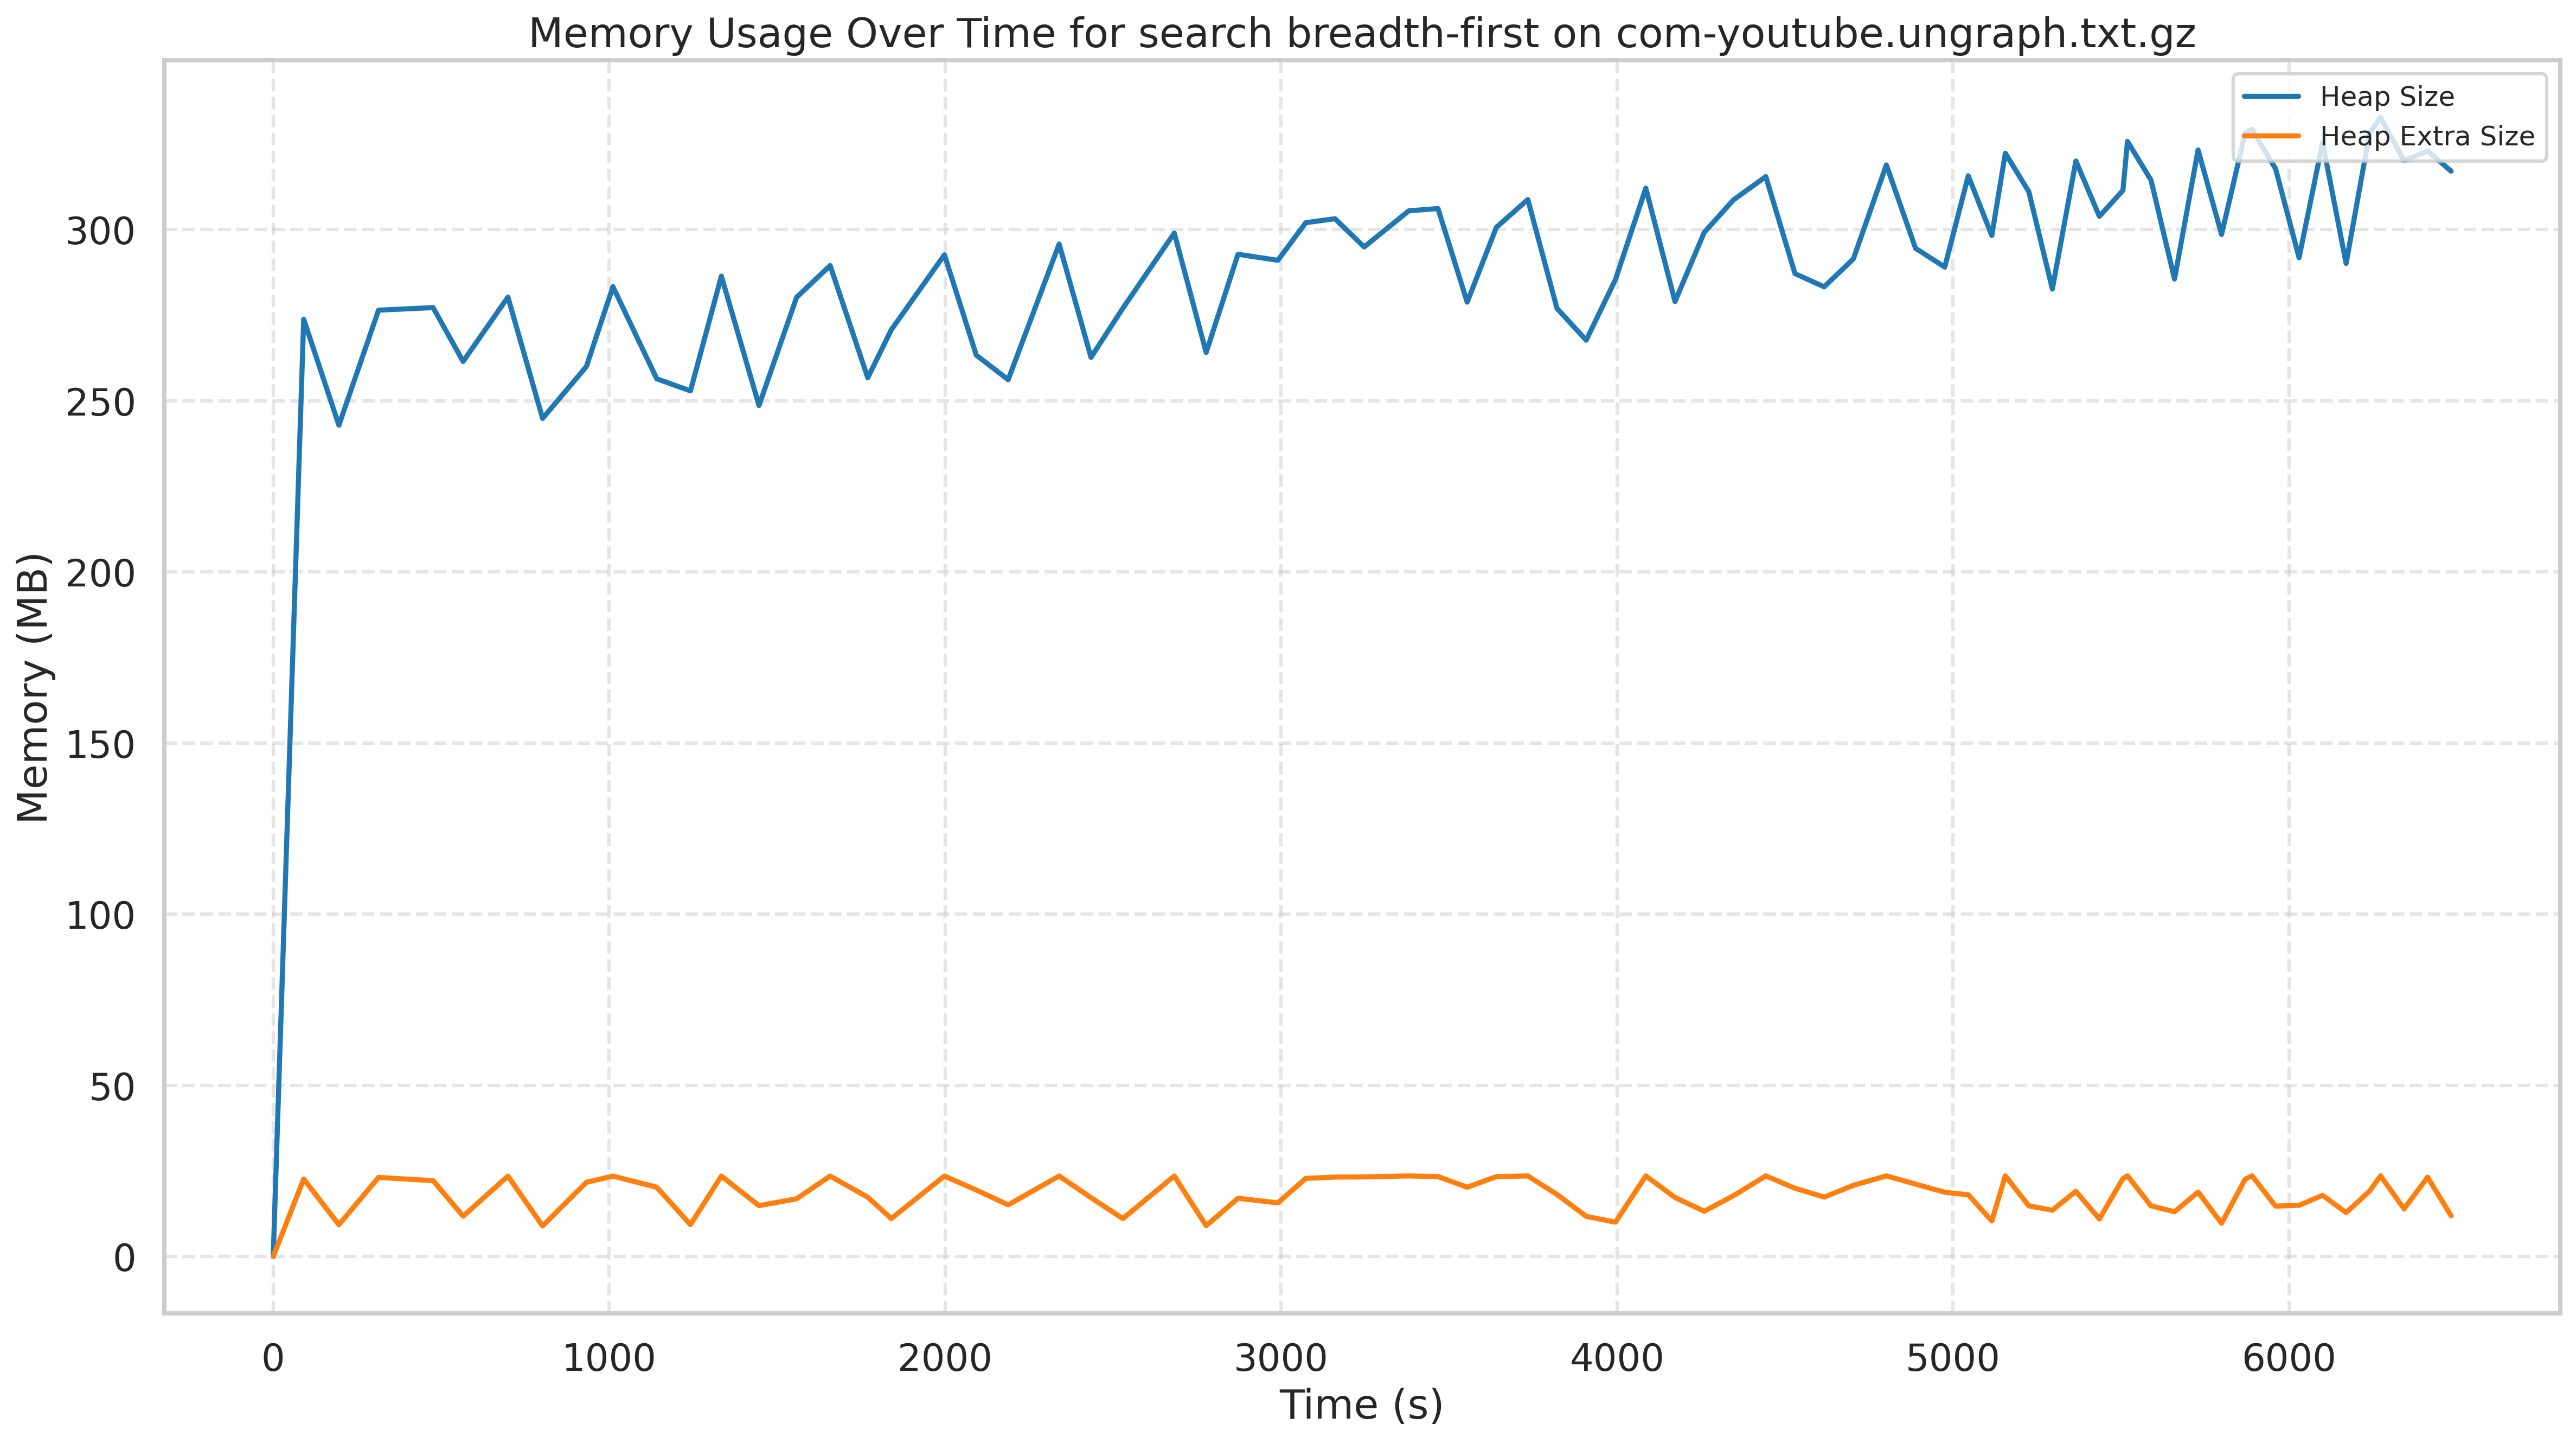
\includegraphics[width=\textwidth]{../plots/com-youtube.ungraph_breadth-first.png}
\caption{Grafico: breadth-first su com-lj.ungraph}
\end{figure}
\subsubsection{Algoritmo di ricerca: uniform-cost}
\begin{figure}[h]\centering
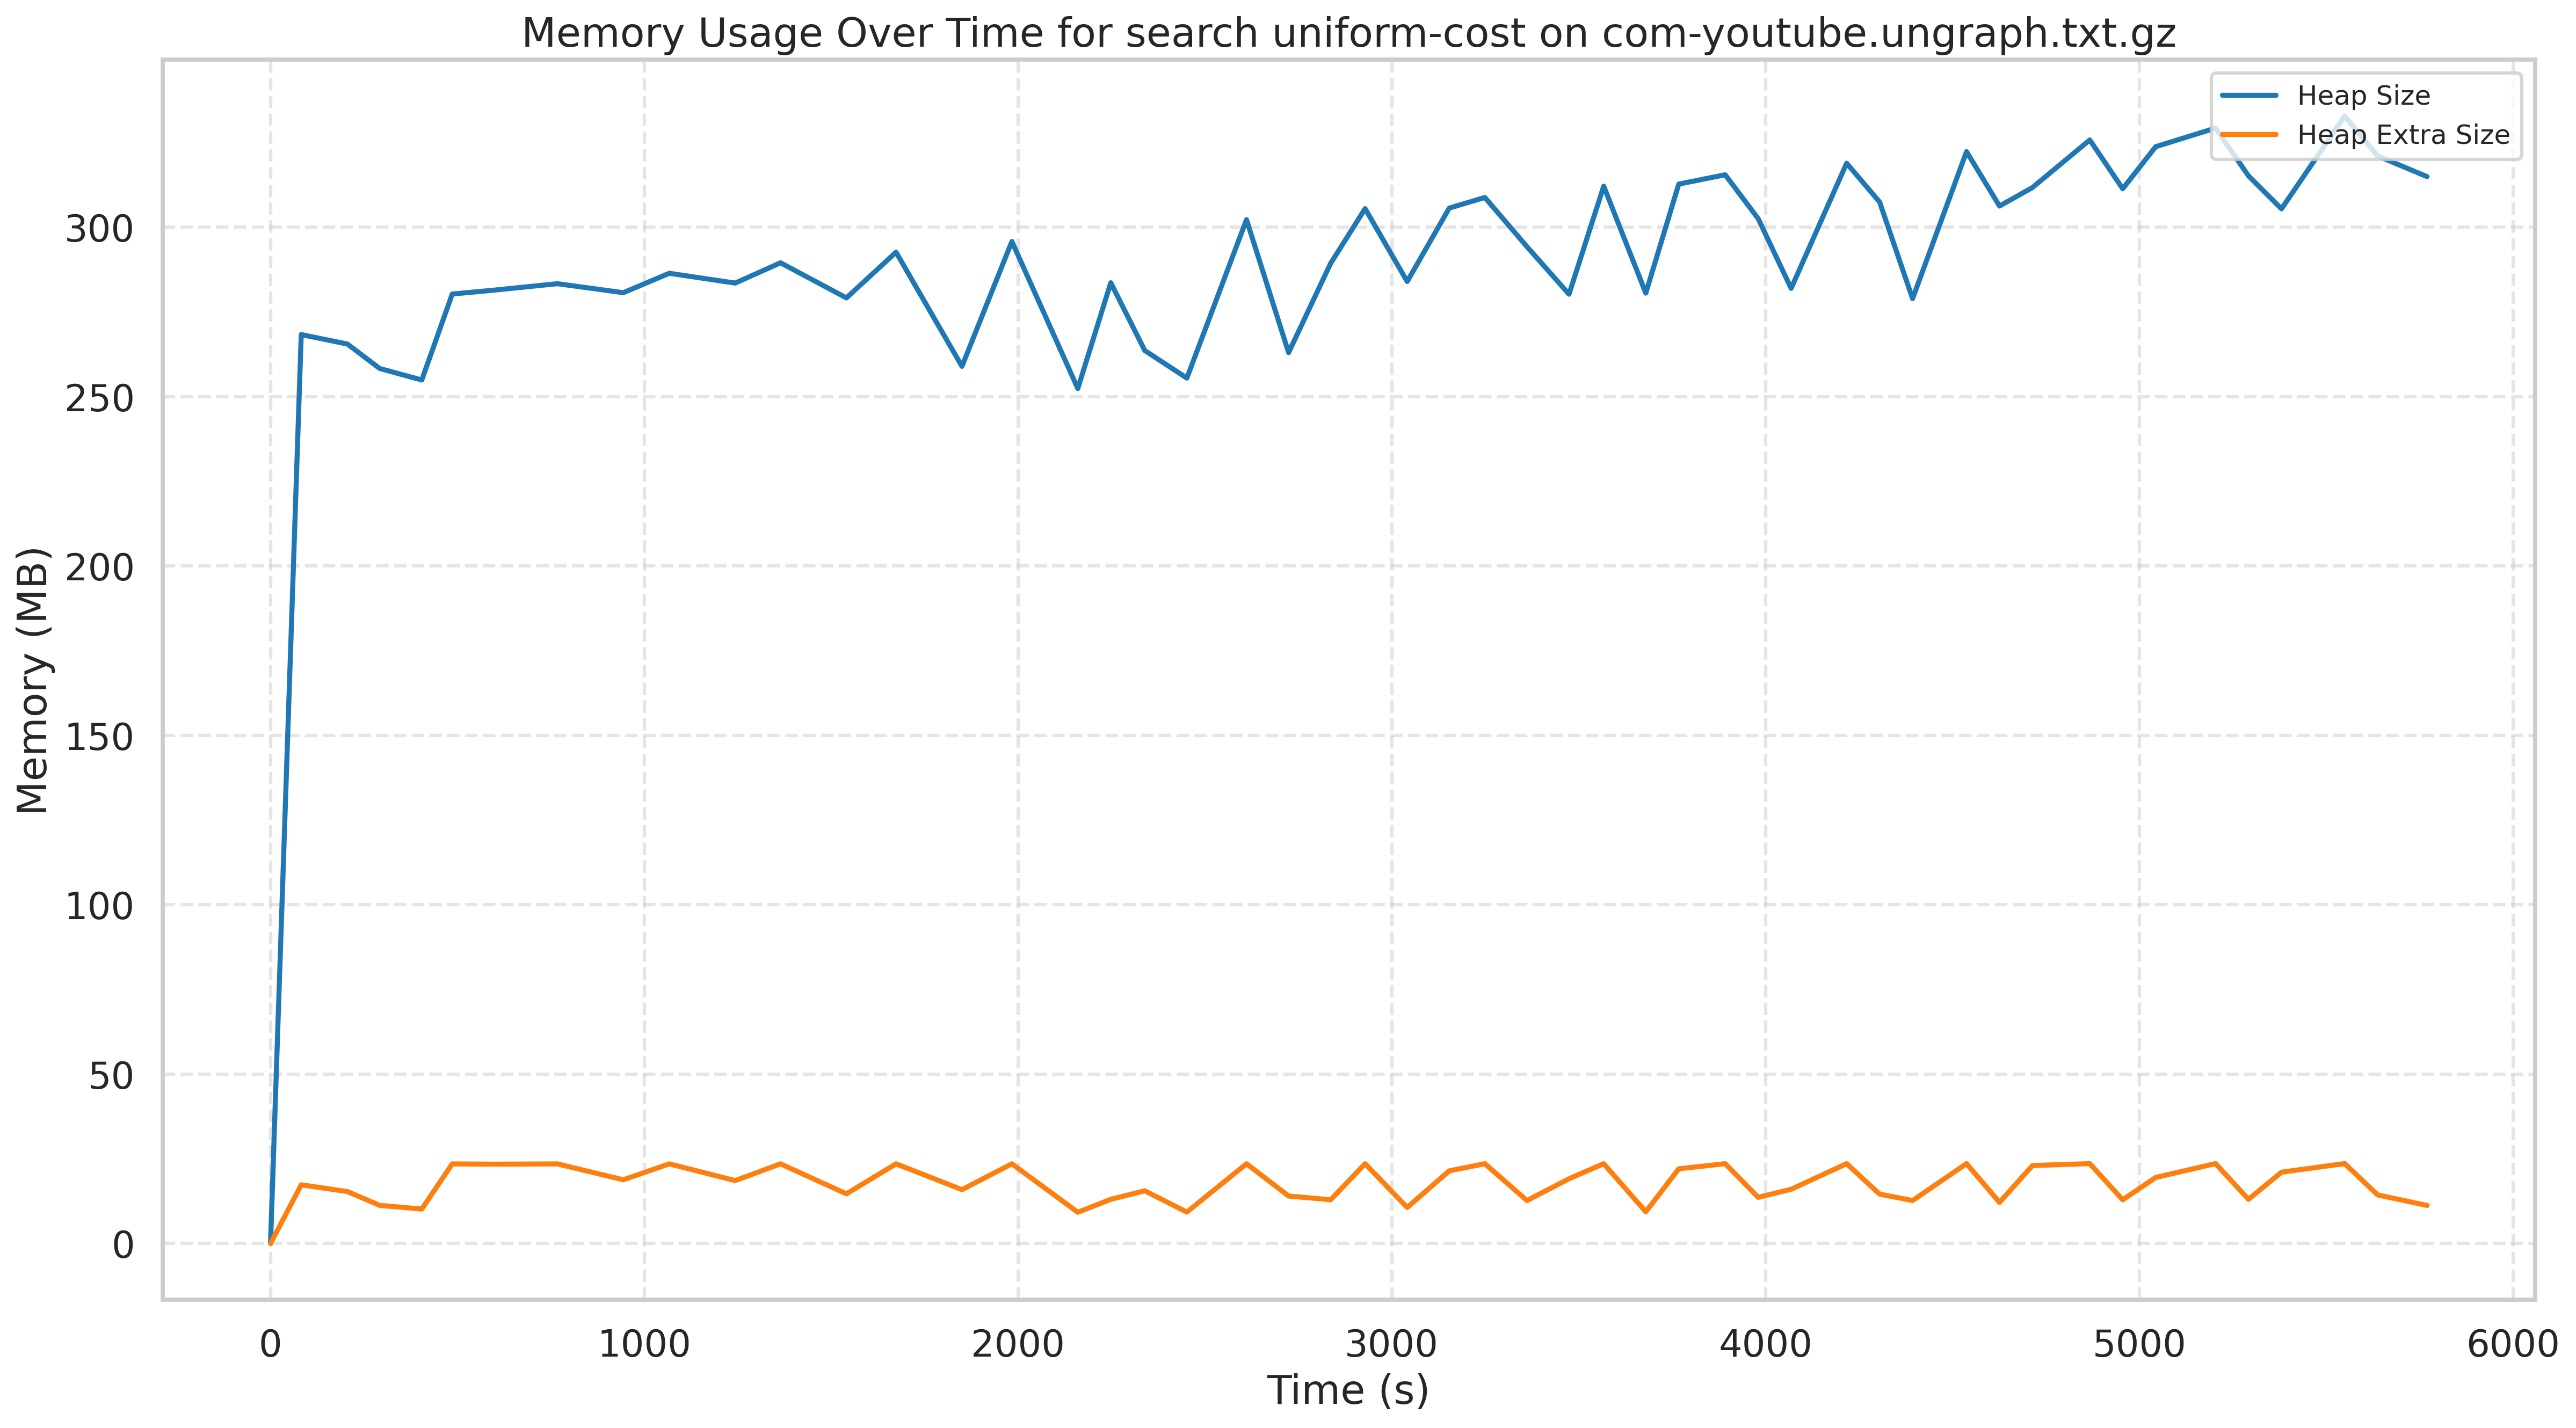
\includegraphics[width=\textwidth]{../plots/com-youtube.ungraph_uniform-cost.png}
\caption{Grafico: breadth-first su com-lj.ungraph}
\end{figure}
\subsubsection{Algoritmo di ricerca: depth-limited}
\begin{figure}[h]\centering
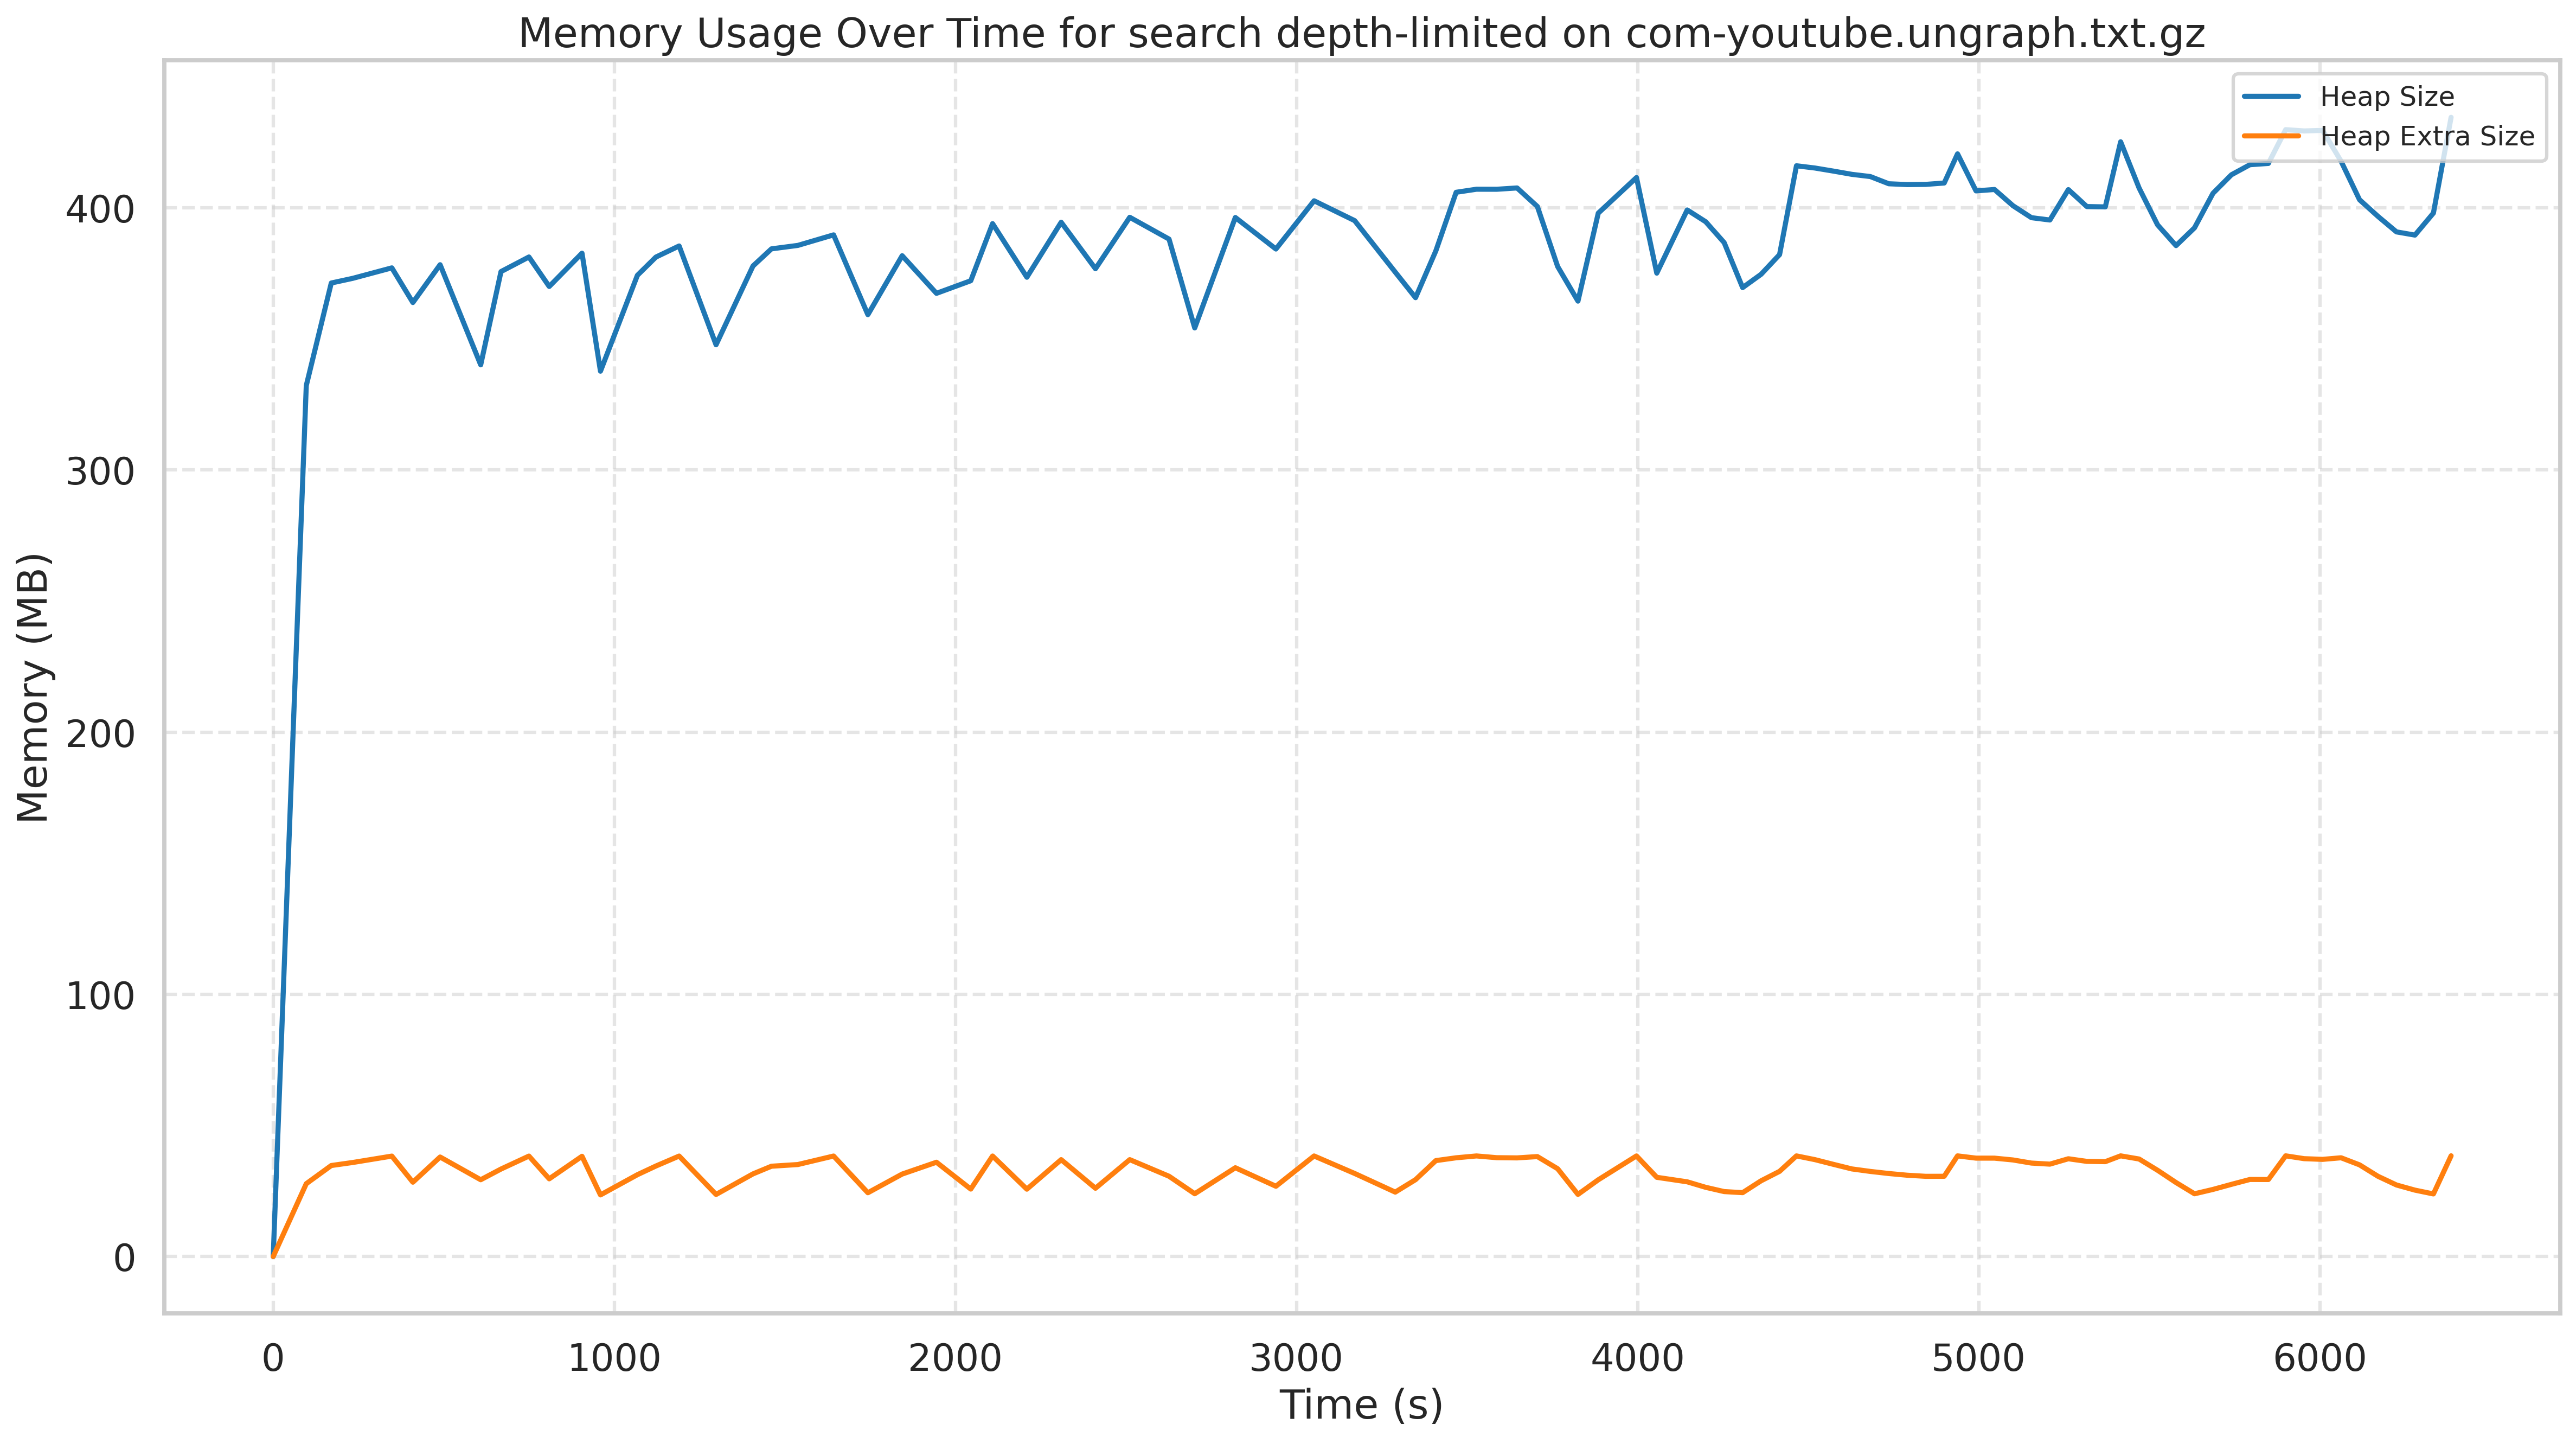
\includegraphics[width=\textwidth]{../plots/com-youtube.ungraph_depth-limited.png}
\caption{Grafico: breadth-first su com-lj.ungraph}
\end{figure}
\subsubsection{Algoritmo di ricerca: iterative-deepening}
\begin{figure}[h]\centering
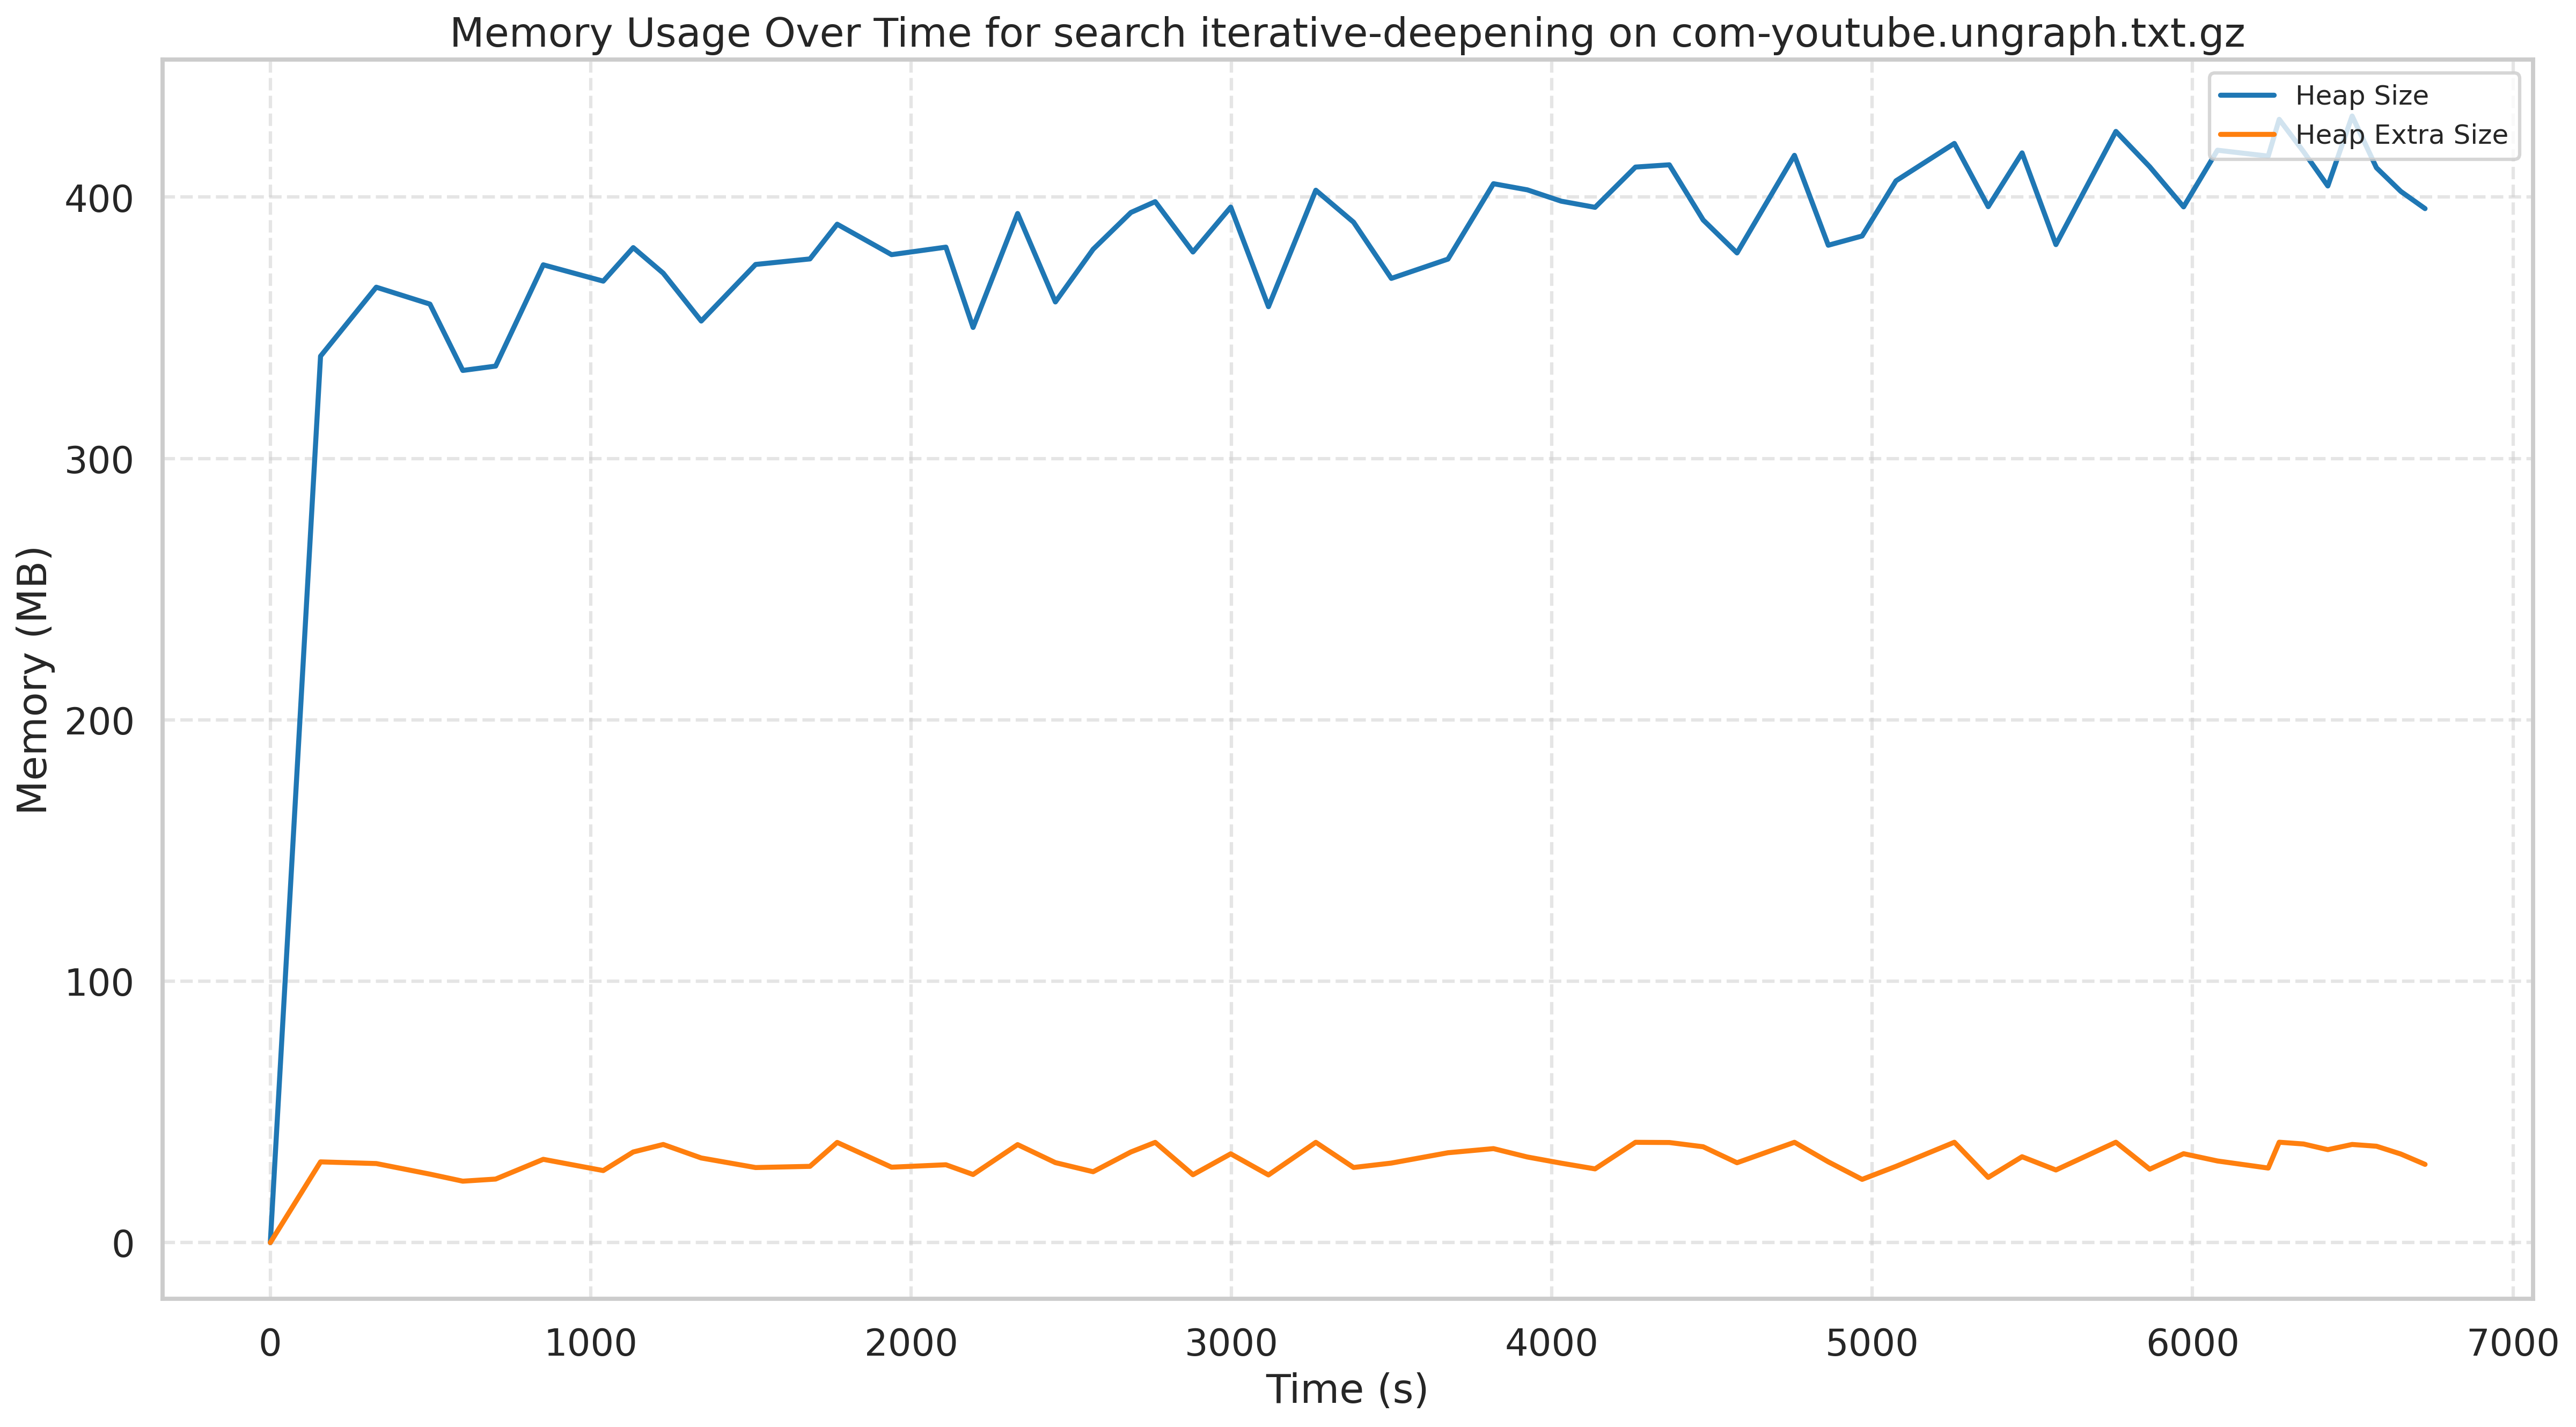
\includegraphics[width=\textwidth]{../plots/com-youtube.ungraph_iterative-deepening.png}
\caption{Grafico: breadth-first su com-lj.ungraph}
\end{figure}
\subsubsection{Algoritmo di ricerca: bi-directional}
\begin{figure}[h]\centering
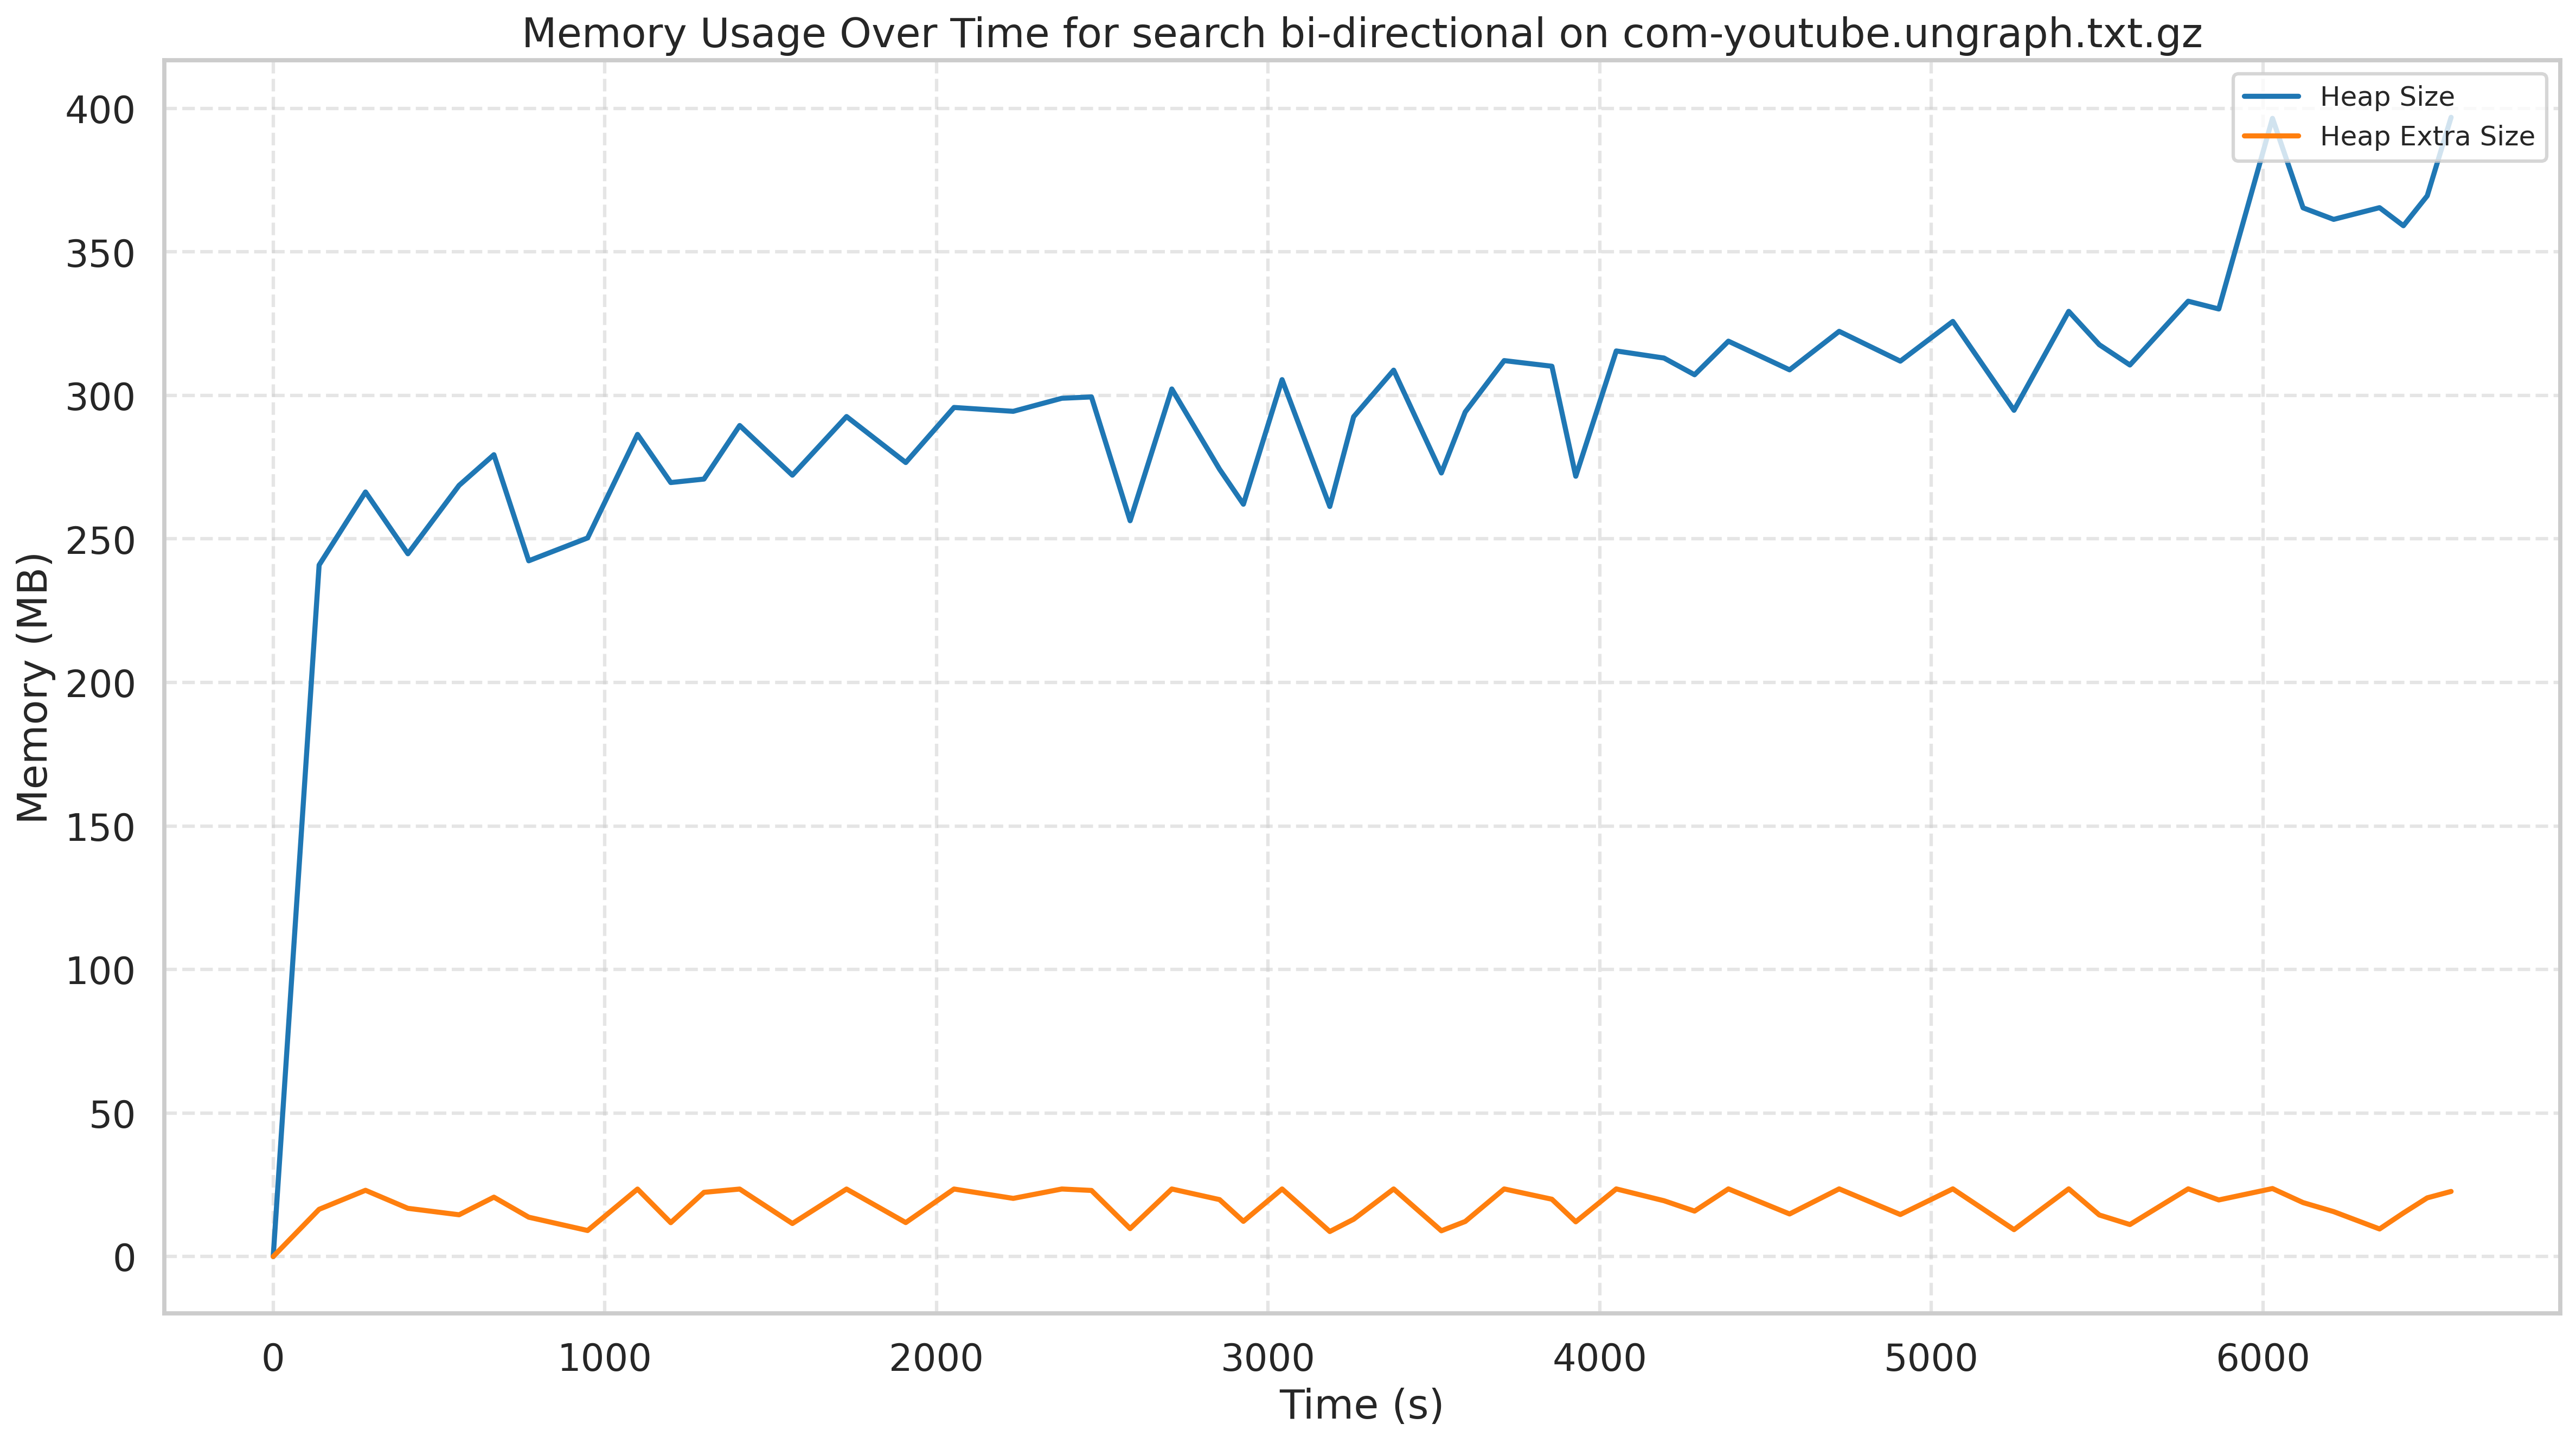
\includegraphics[width=\textwidth]{../plots/com-youtube.ungraph_bi-directional.png}
\caption{Grafico: breadth-first su com-lj.ungraph}
\end{figure}
\subsubsection{Algoritmo di ricerca: breadth-first}
\begin{figure}[h]\centering
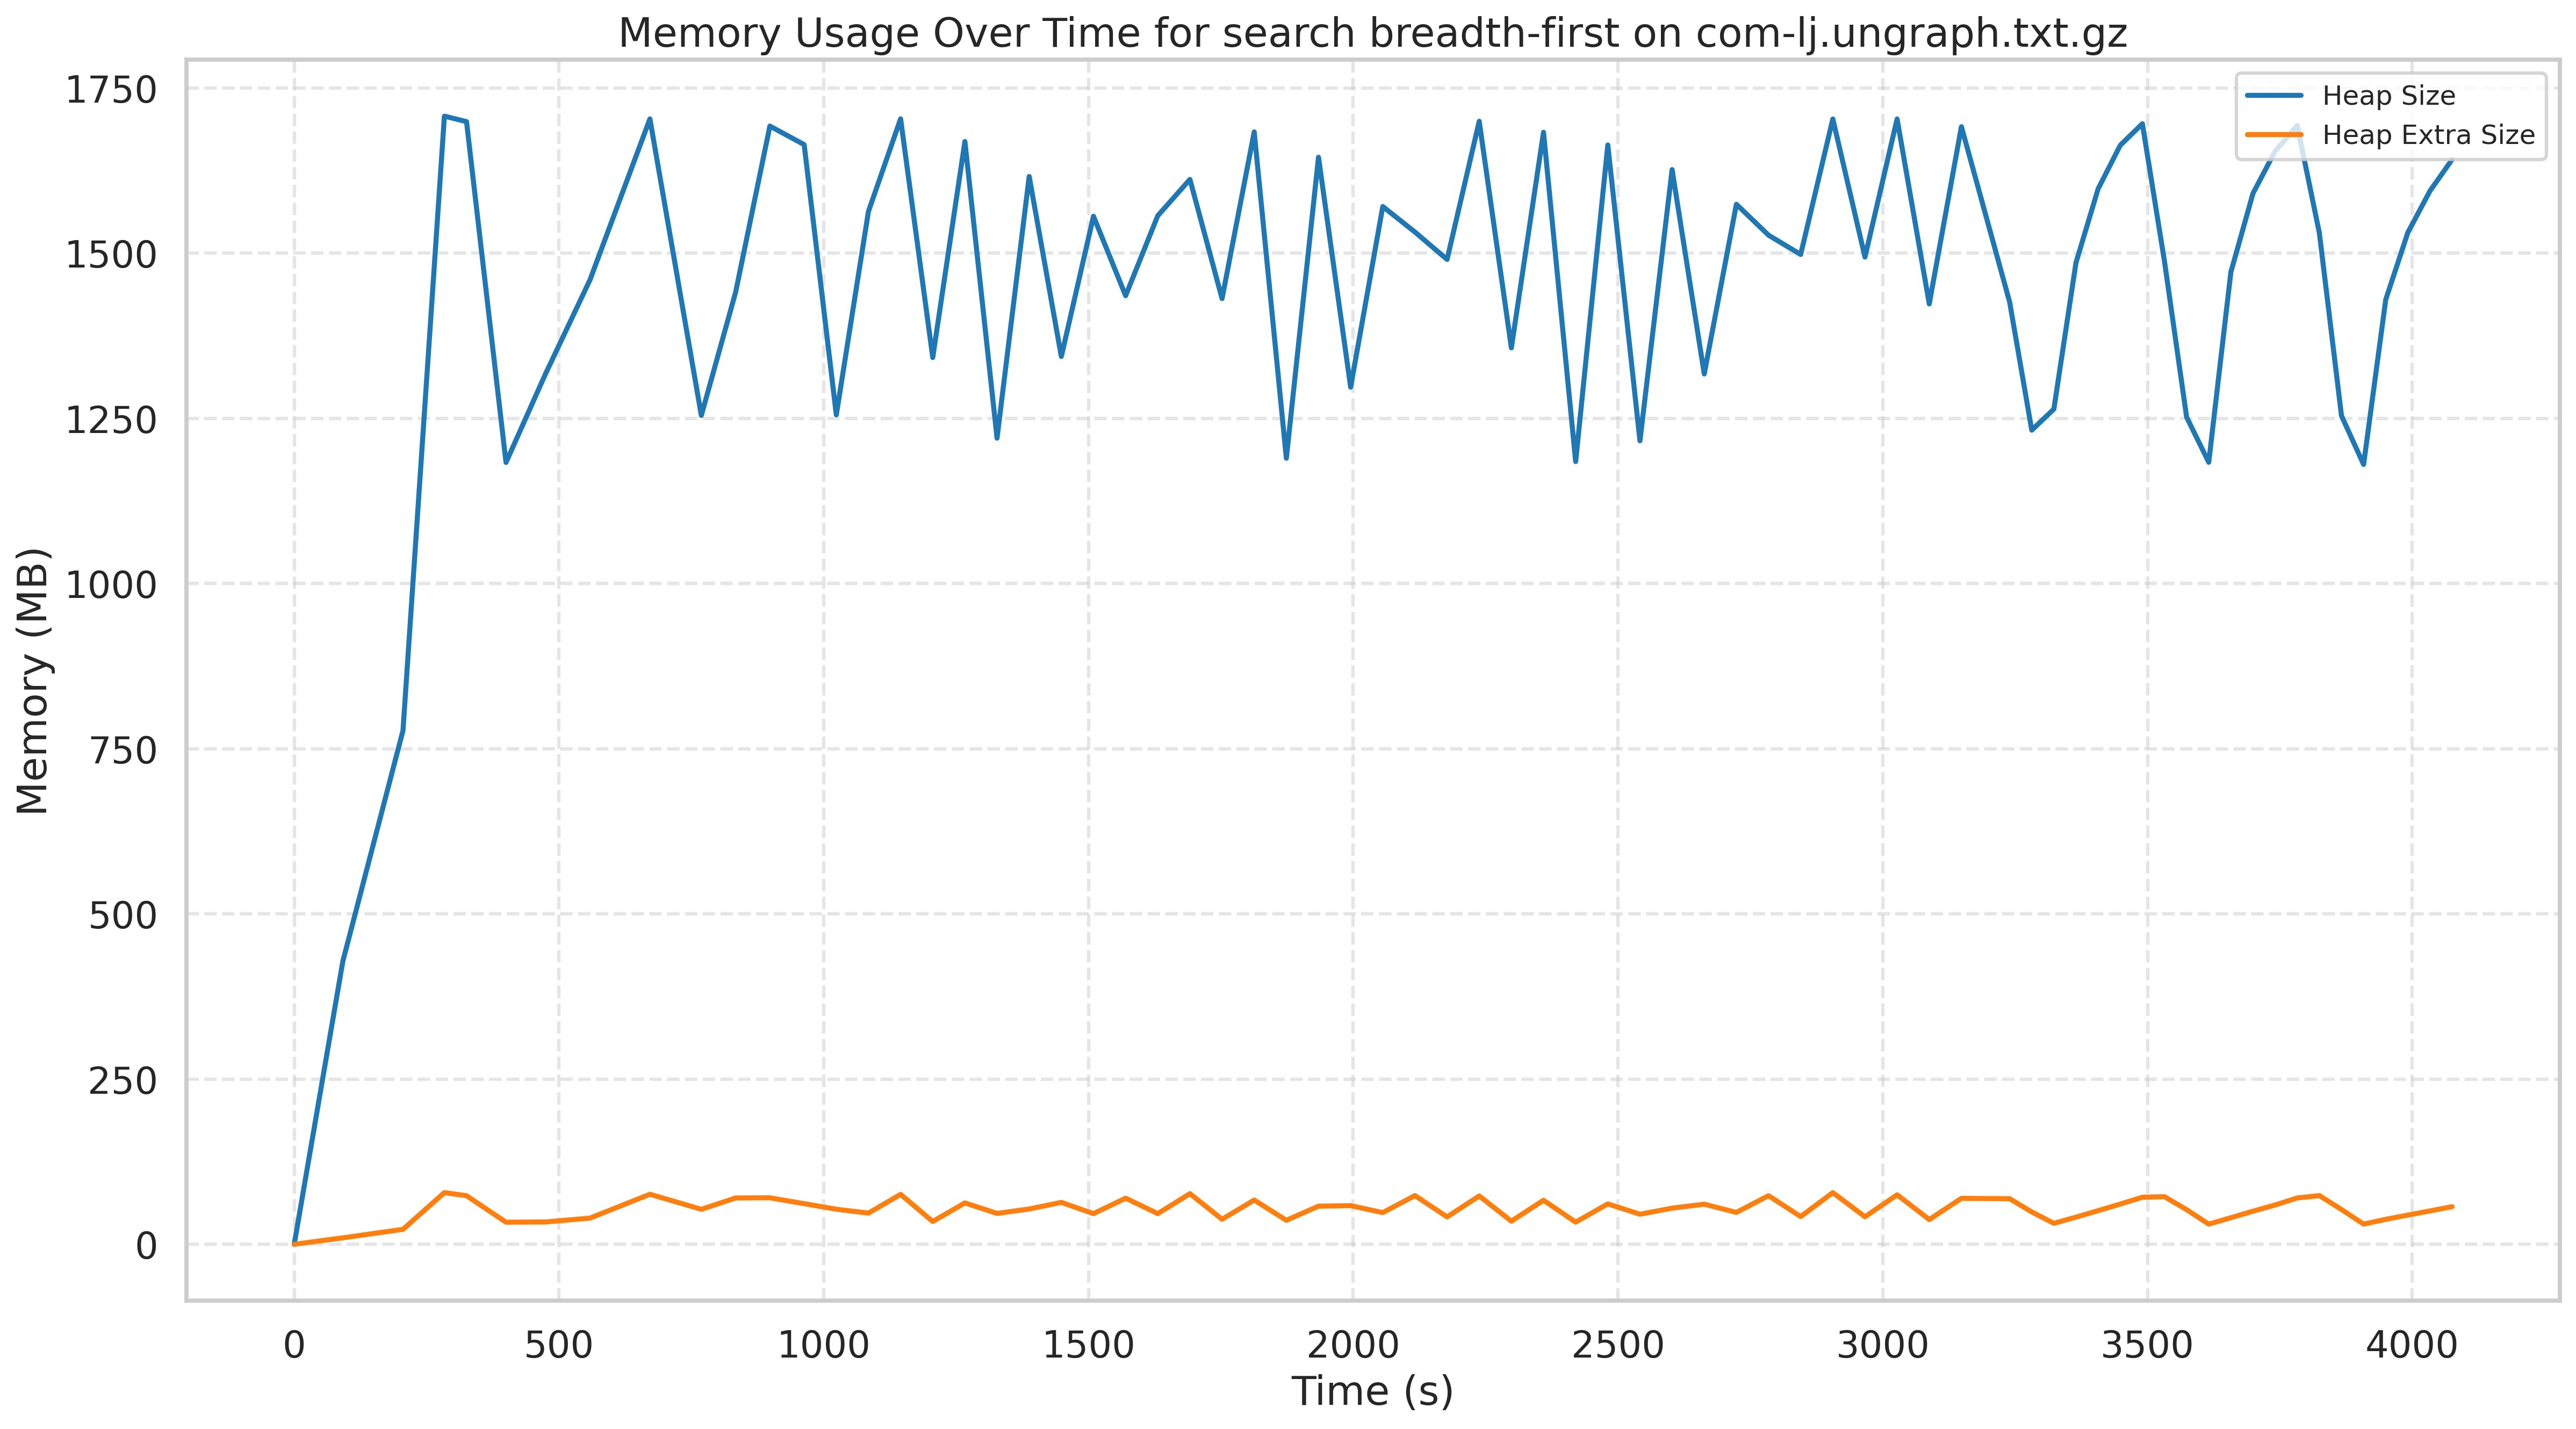
\includegraphics[width=\textwidth]{../plots/com-lj.ungraph_breadth-first.png}
\caption{Grafico: breadth-first su com-lj.ungraph}
\end{figure}
\subsubsection{Algoritmo di ricerca: uniform-cost}
\begin{figure}[h]\centering
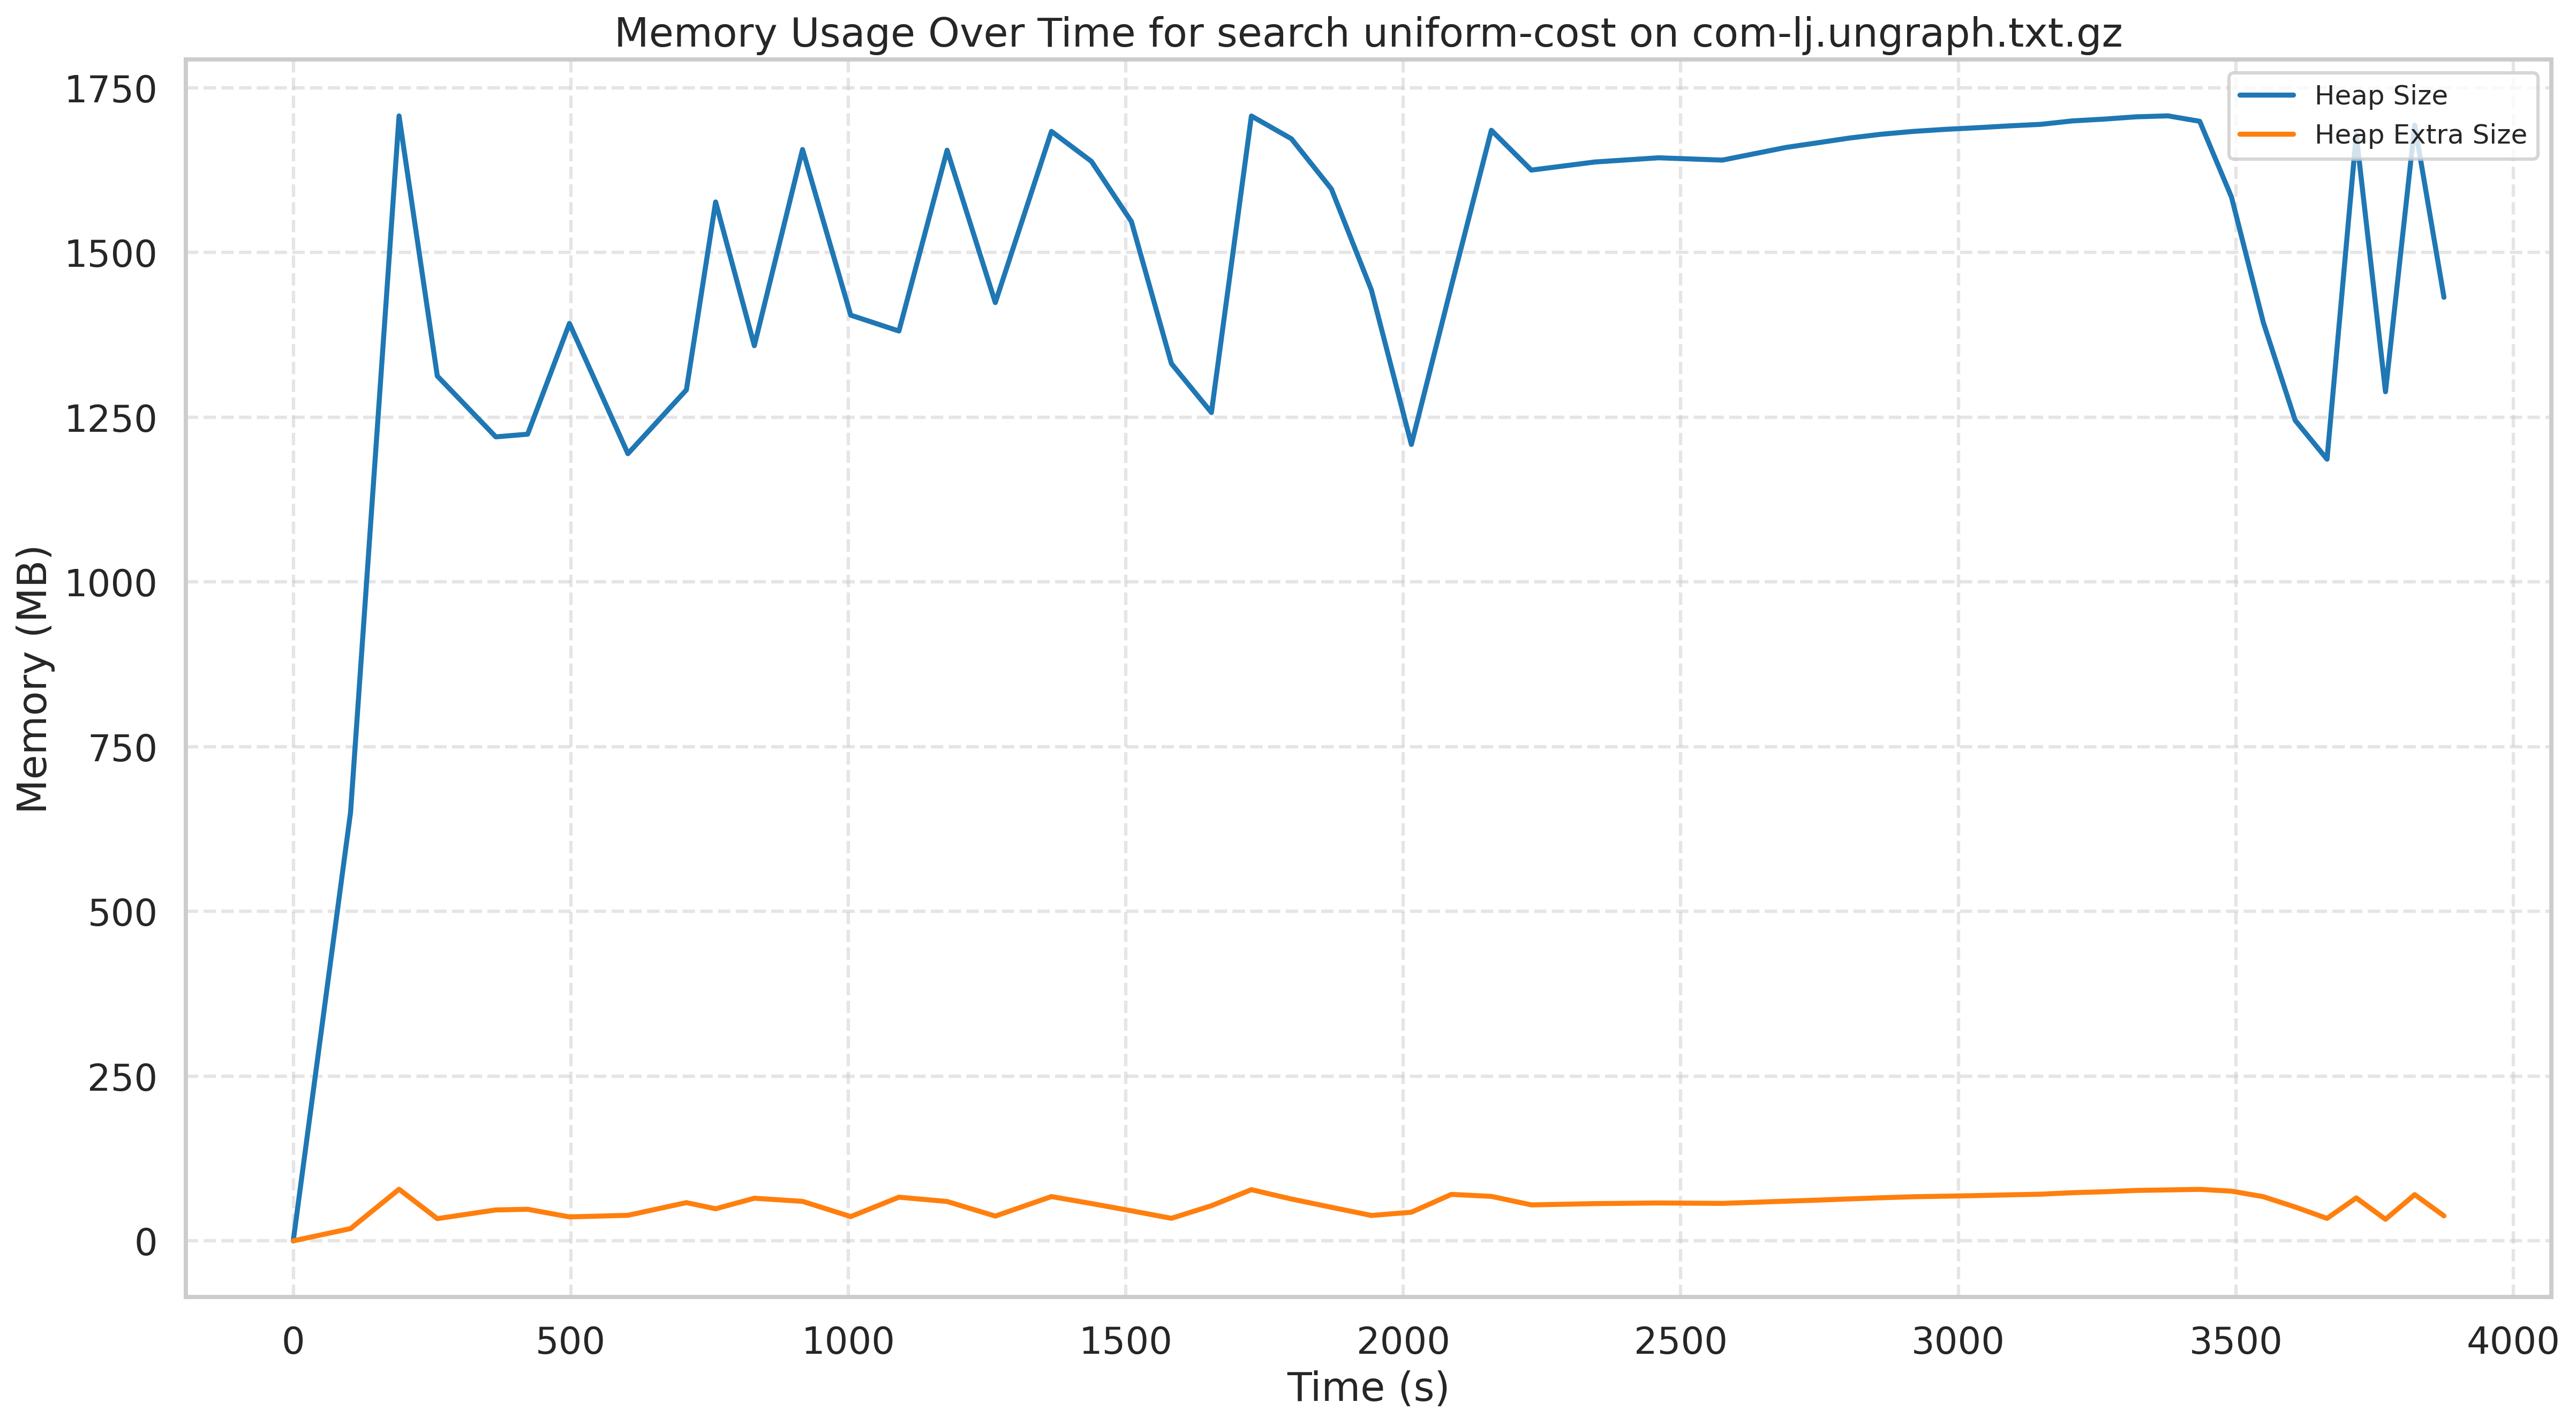
\includegraphics[width=\textwidth]{../plots/com-lj.ungraph_uniform-cost.png}
\caption{Grafico: breadth-first su com-lj.ungraph}
\end{figure}
\subsubsection{Algoritmo di ricerca: depth-limited}
\begin{figure}[h]\centering
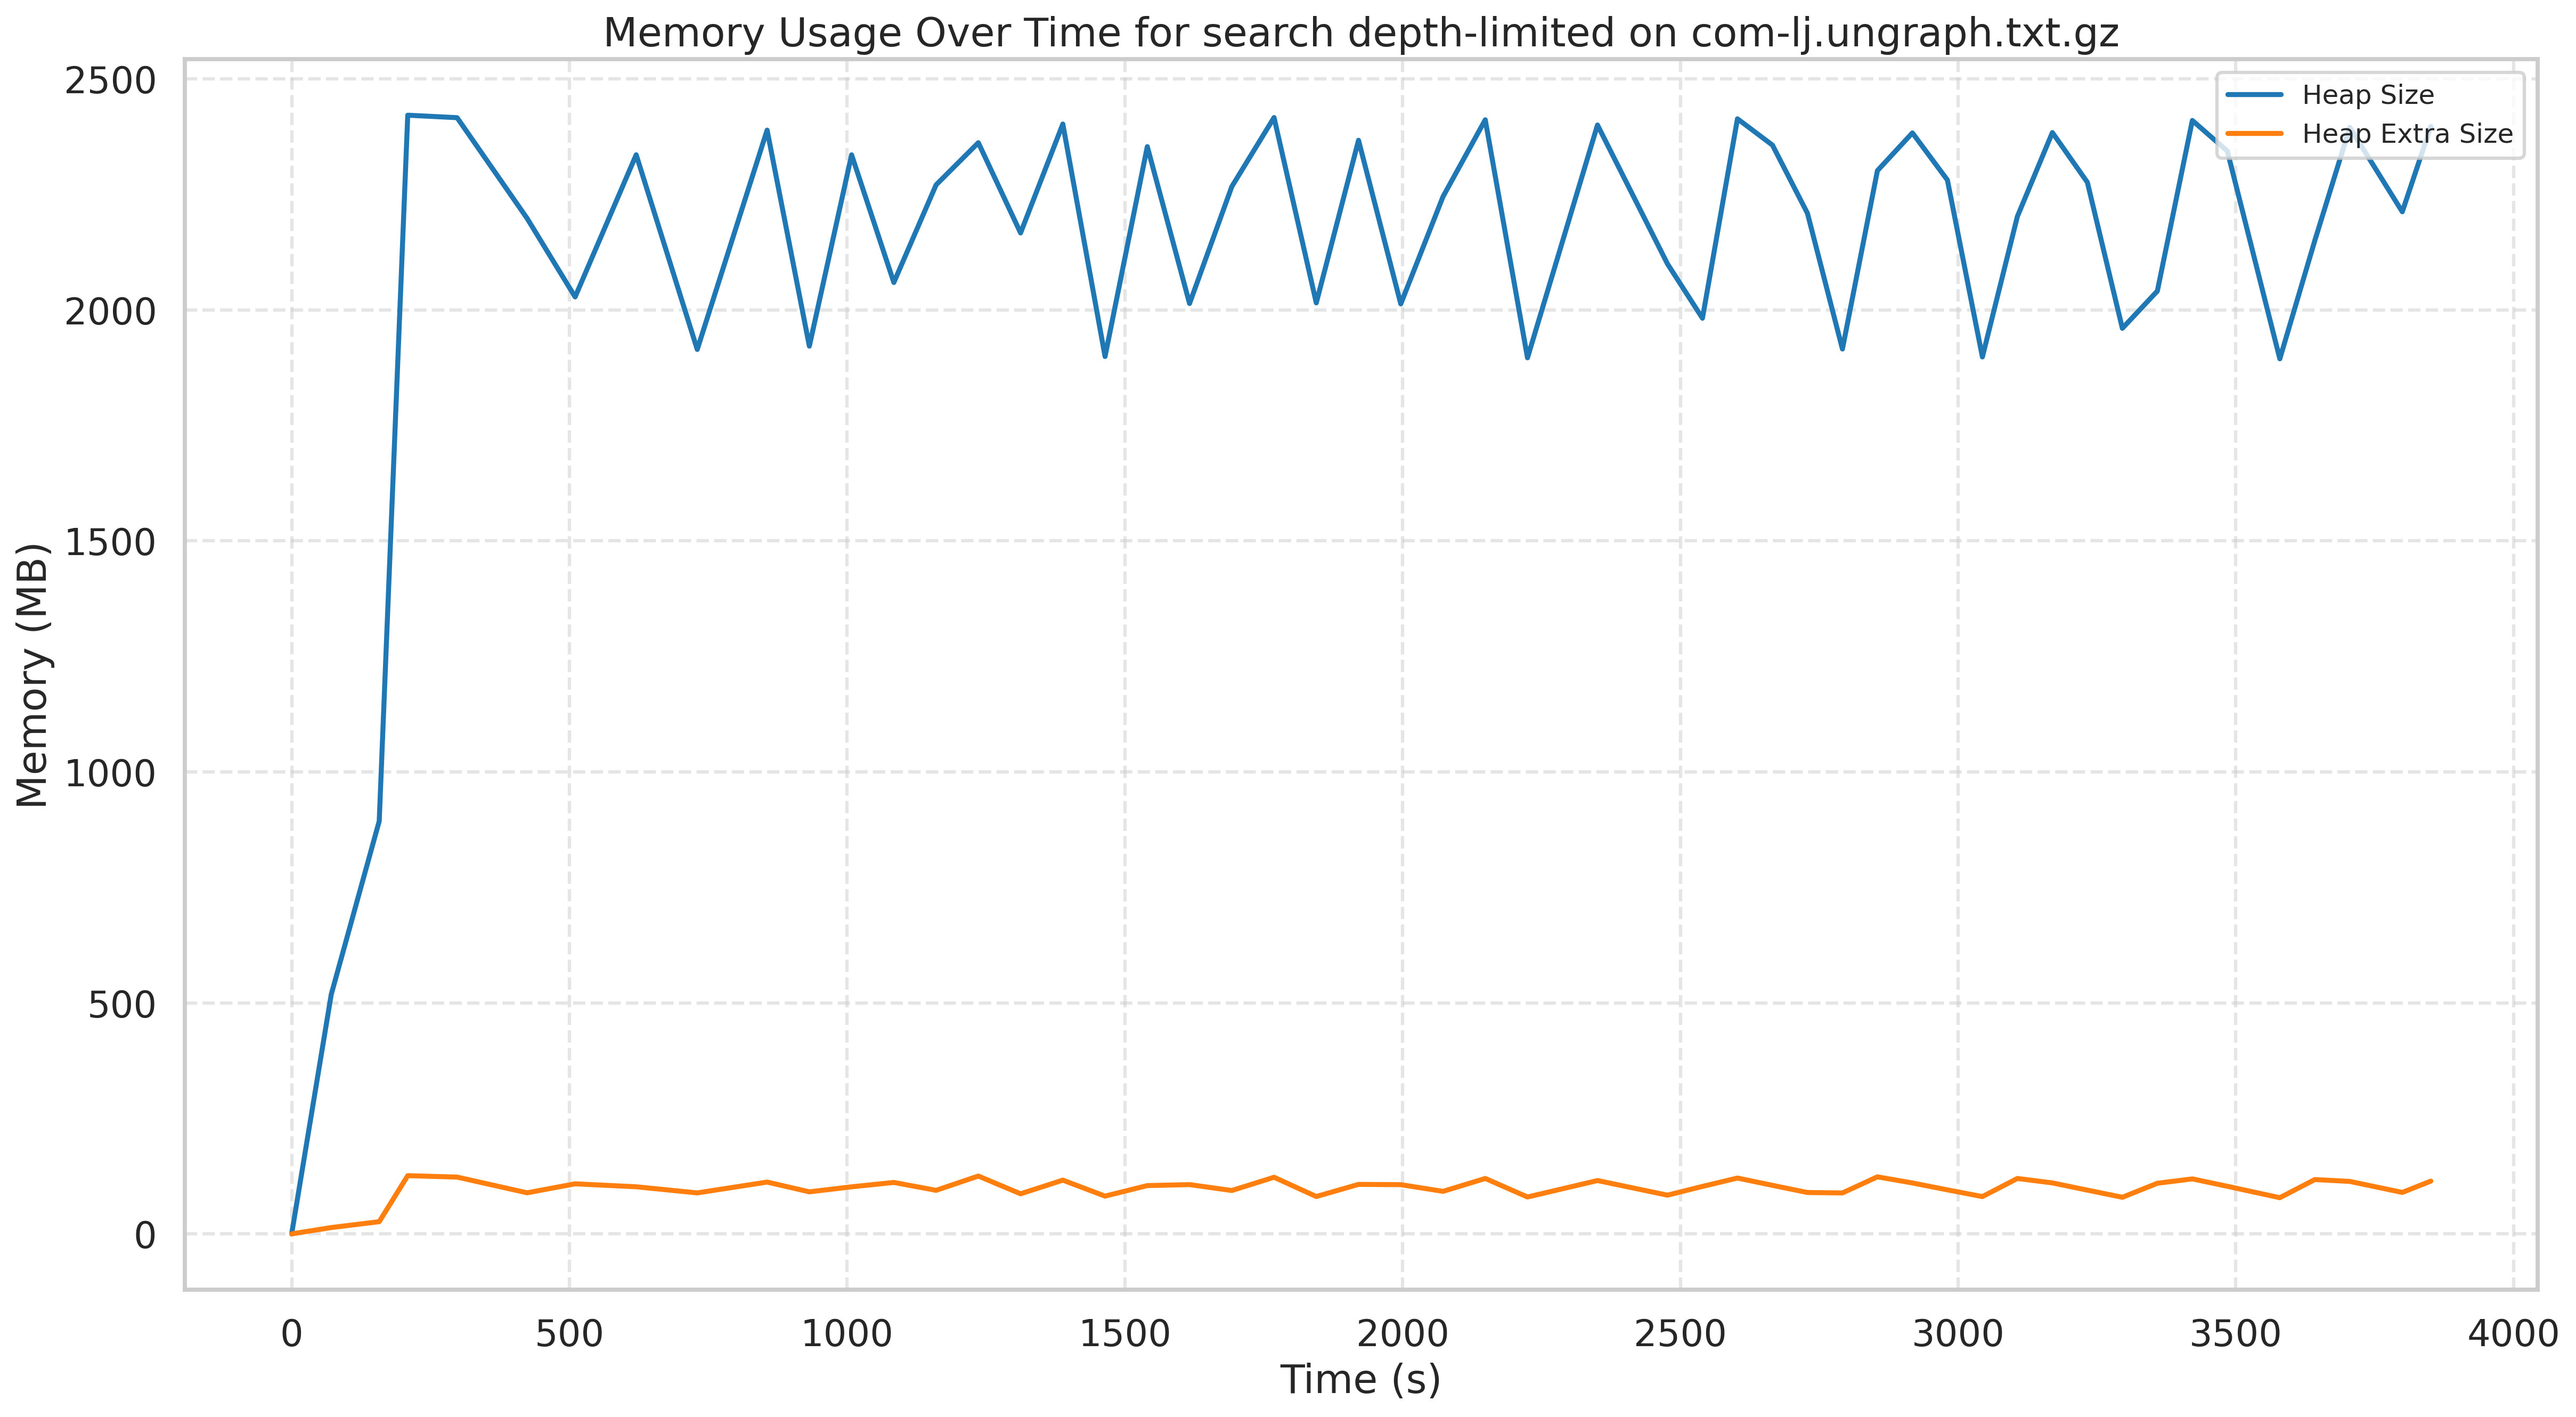
\includegraphics[width=\textwidth]{../plots/com-lj.ungraph_depth-limited.png}
\caption{Grafico: breadth-first su com-lj.ungraph}
\end{figure}
\subsubsection{Algoritmo di ricerca: iterative-deepening}
\begin{figure}[h]\centering
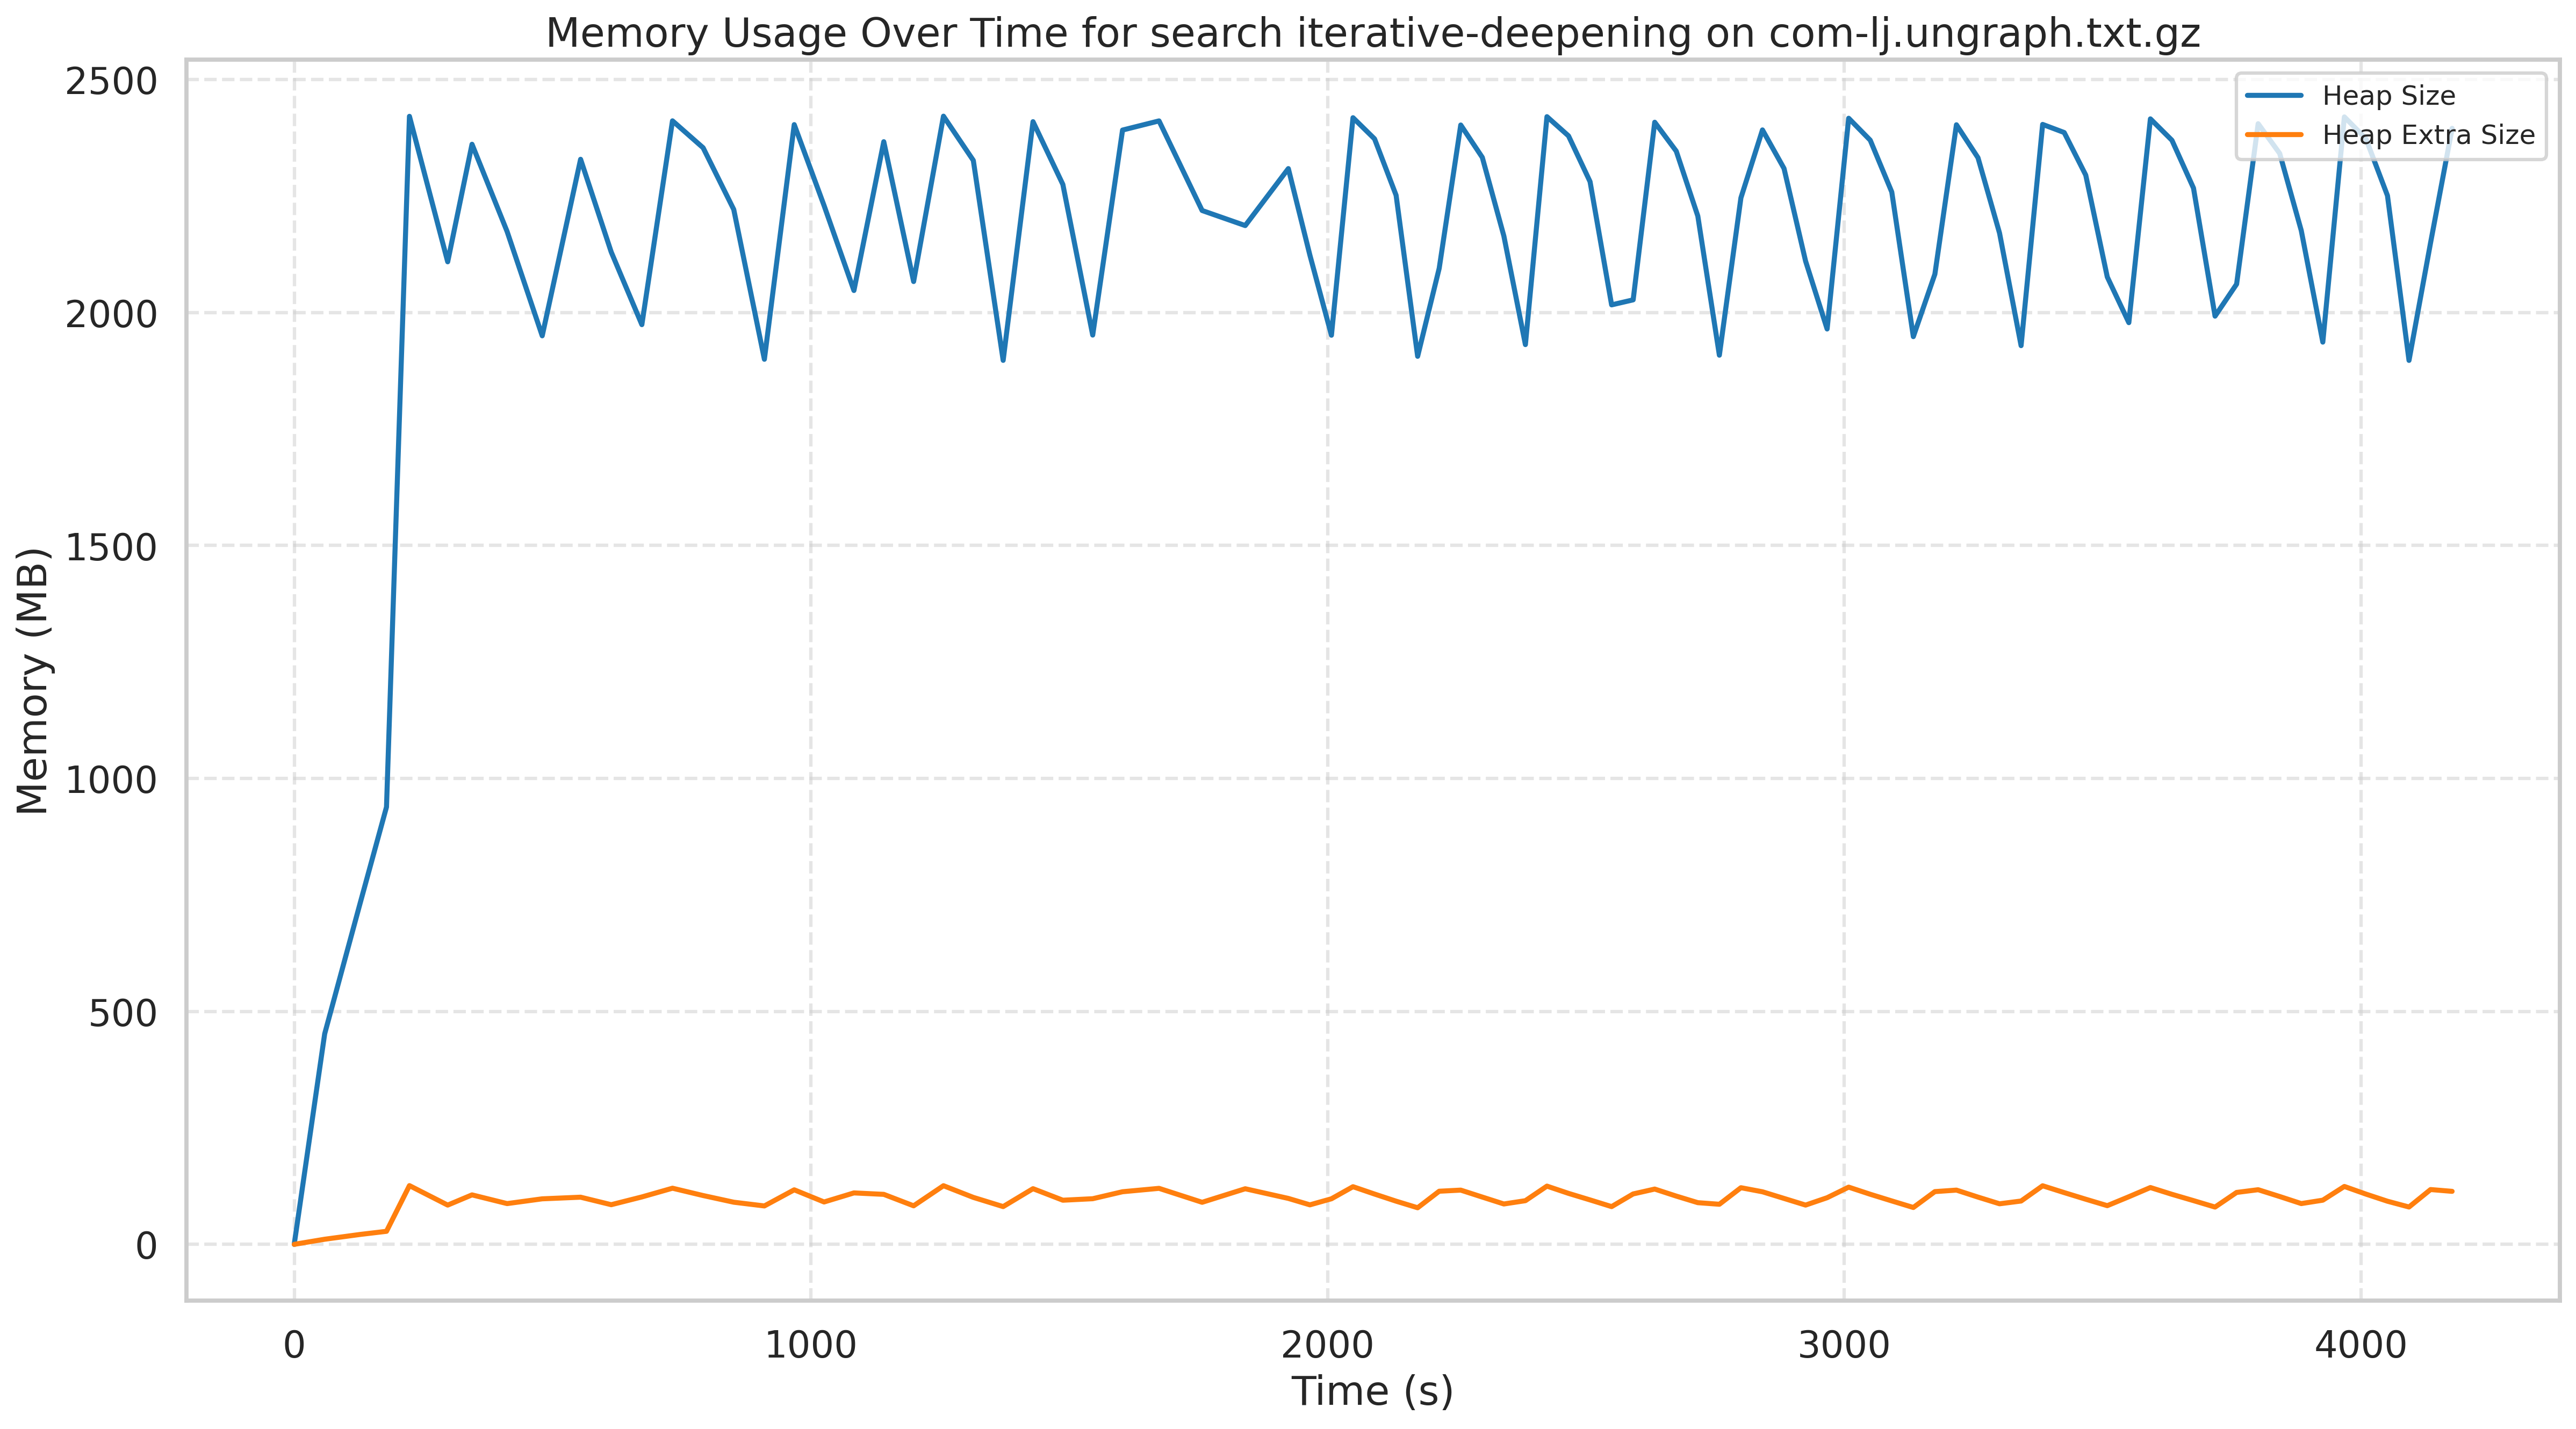
\includegraphics[width=\textwidth]{../plots/com-lj.ungraph_iterative-deepening.png}
\caption{Grafico: breadth-first su com-lj.ungraph}
\end{figure}
\subsubsection{Algoritmo di ricerca: bi-directional}
\begin{figure}[h]\centering
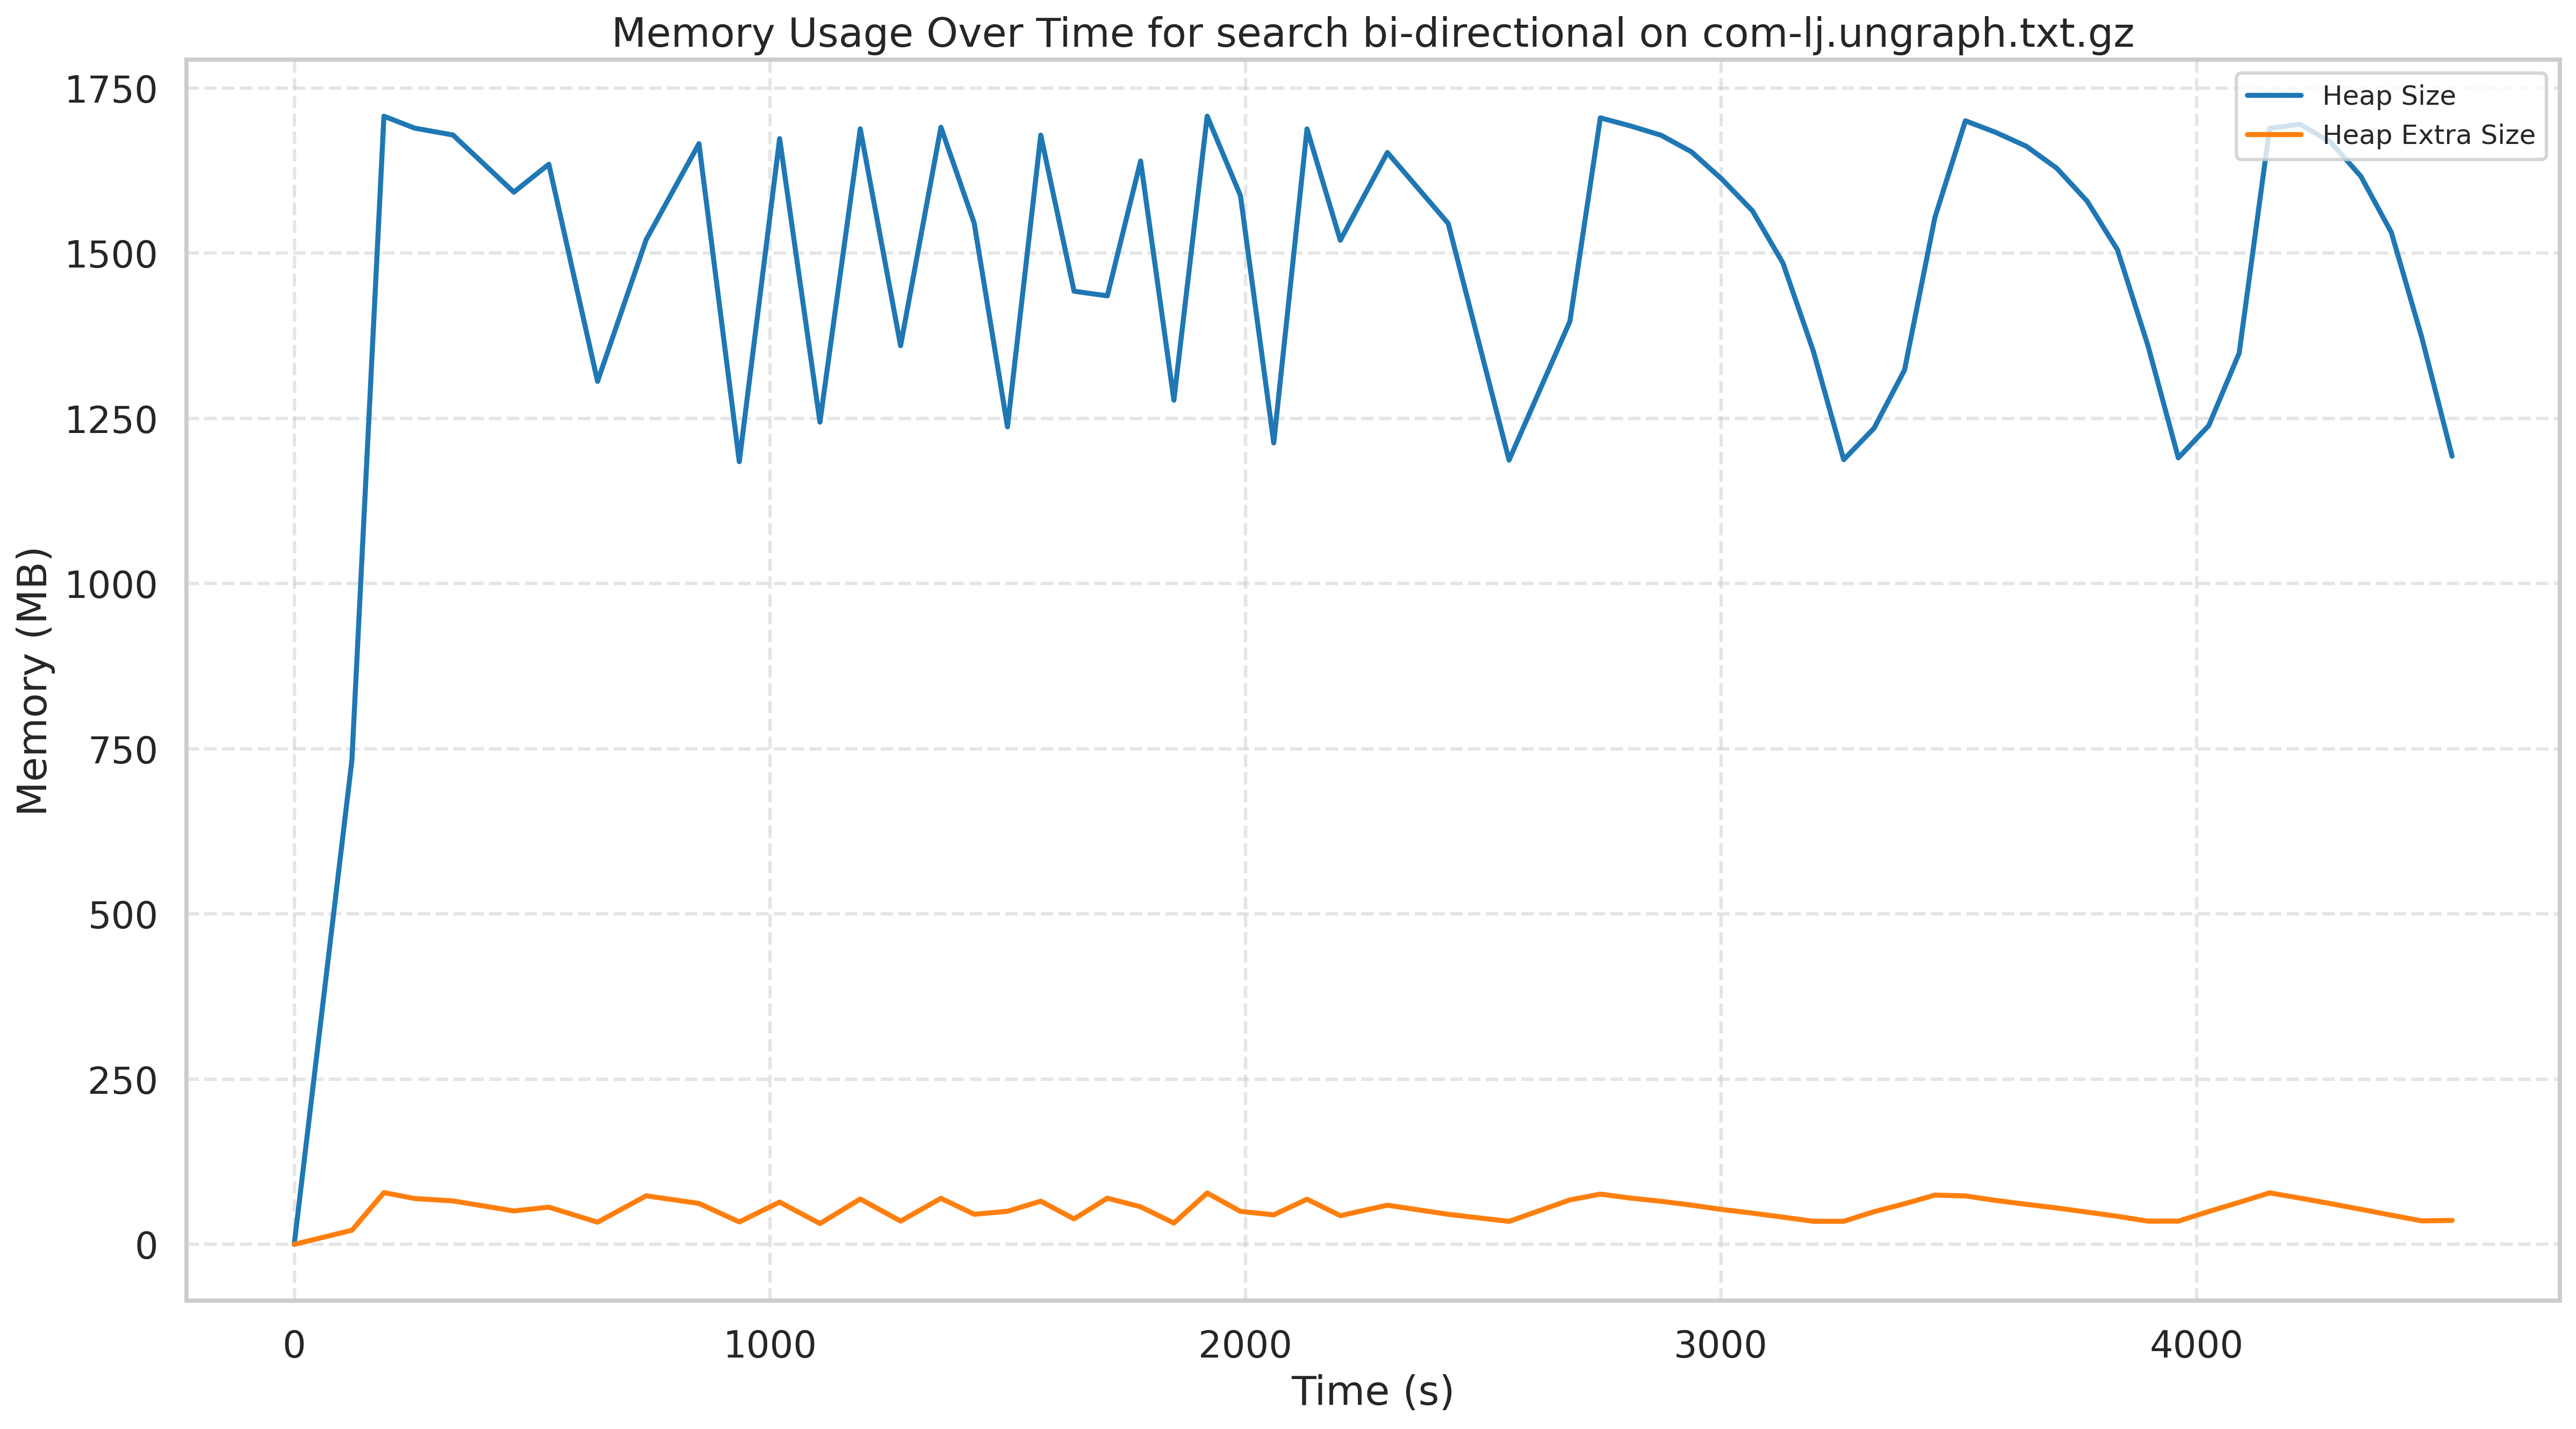
\includegraphics[width=\textwidth]{../plots/com-lj.ungraph_bi-directional.png}
\caption{Grafico: breadth-first su com-lj.ungraph}
\end{figure}
\end{document}